%\chapter {MetaTracts - Robust Extraction and Visualization of Fiber Bundles in Fiber Reinforced Composites}
%\label{metaTracts.ch}



\section{Introduction and Motivation}
\label{sec:intro}
Modern industry is increasingly demanding function orientation, integration, and efficiency of novel materials and components. The material of choice for a growing number of applications is carbon fiber reinforced polymer (CFRP), which allows an integration of these continuously rising demands and increasingly replaces conventional materials such as aluminum or steel. 
%CFRPs have been successfully introduced in aeronautic and automotive %applications within recent years, replacing parts made of conventional %materials such as aluminum or steel. But the application areas of CFRPs %are not limited on these two industries. For a wide range of different %areas ranging from marine and civil engineering, wind energy, to sporting %goods manufacturing, CFRP is highly interesting. 
%The main reason therefore is found in CFRP materials having desirable %characteristics such as high specific stiffness, high specific strength %and high corrosion resistance. 
CFRP materials have desirable characteristics such as high specific stiffness, high specific strength and high corrosion resistance. Moreover, CFRP materials show these characteristics at considerably lower weight. At the same time, highly complex and integrated components, which were previously impossible to manufacture may be produced from CFRPs. Primary structures and highly loaded components in aeronautics are one example.
Typically, carbon fiber reinforced polymer components and more specifically CFRP laminates with endless carbon fibers as addressed in this work consist of two main components:
a matrix, which acts as a bonding component, and the reinforcements, which allow for achieving the desired characteristics. Various production processes are used to manufacture CFRP laminates. Most of these processes start with the reinforcement component, weaving individual carbon fiber bundles (yarn) into sheets of carbon fiber cloth in a predefined pattern. These sheets of woven carbon fiber cloth are also referred to as fabric and form the geometrical structure of the final CFRP materials. Depending on the requirements of the final component, fabrics may be stacked in multiple layers in similar or different orientation. Both alignment of fabrics and the weaving pattern of the individual carbon fiber bundles strongly influence the properties of the CFRP laminate. Resins are then integrated in the material system to fill the gaps in the fabric forming the matrix component. The main function of the matrix is to act as a bonding between the individual carbon fiber bundles. After curing, the production process of the CFRP laminate is finished. 

The increasing share of CFRPs as well as the complexity of both material system and final component has generated a strong demand towards non-destructive testing (NDT) techniques for quality control~\cite{Red2012}. Ultrasonic testing (UT) is the most commonly used method for this purpose. While UT provides a quick and cost-efficient overview of the material, it also lacks resolution and may generate arbitrary results, e.g., due to the geometry of the component. Industrial 3D X-ray computed tomography (XCT, also referred to as 3DXCT or cone beam XCT) is increasingly applied for non-destructive testing of fiber reinforced polymers~\cite{Kastner2012}. In contrast to UT, XCT generates a highly detailed 3D volumetric representation of the scanned specimen. In cone beam XCT geometry the specimen is placed on a rotary table between X-ray source and detector. The X-rays passing through the specimen get attenuated by the materials present. By transferring the X-rays in a scintillator layer into visible light, the detector records the corresponding 2D attenuation image (penetration image). The specimen is rotated recording at each angular step a 2D attenuation image to generate the full series of attenuation images of a $360^\circ$ rotation required for a complete reconstruction of the data volume ~\cite{heinzl-2008-thesis}. 
While cone beam XCT can reach voxel sizes below 500 $nm$ generating high resolution volume data for comprehensive and detailed analyses, unfortunately there is still a trade-off between viewport and image resolution. The magnification reached within an XCT scan is determined by the used distances between source and specimen as well as source and detector. The magnification therefore directly influences both resolution and viewport: while higher resolutions decrease the viewport but show more details, lower resolutions allow for larger viewports and thus larger portions of the specimen.

In this work, we focus on datasets with larger viewports but lower resolutions where the individual carbon fibers (filaments) are indiscernible or barely visible. Our domain experts are mainly interested in visualizing the geometric structures in the weaving pattern of fiber bundles in endless carbon fiber reinforced composites instead of high resolution studies of individual fibers.
%of short fiber reinforced composites as presented by Weissenbock2014 et al.~\cite{Weissenbock2014}.
Figure~\ref{fig:data-char} depicts our targeted dataset type. It shows the recurring fiber bundle pattern in the final CFRP laminate, the \textit{unit cell}.
Our work is motivated from the recent progress in two interrelated fields: Firstly, CFRP components have gained wide application in industry because of its superior material and physical properties in comparison to conventional materials~\cite{Karpat2012}. Secondly, recent developments of industrial 3D X-ray computed tomography (XCT) with regard to larger detectors, larger field of views, and better resolutions opened XCT for this new application area of NDT for fiber reinforced components~\cite{Schilling2005}. 
%
% Fiber bundles determine to a large extent the properties in terms of specific stiffness, specific strength, or durability of the final component. However, when scanning reinforced polymers using modern XCT devices, there is still a trade-off between view port and image resolution. Due to the intrinsic concept of cone beam and fan beam XCT setups, the magnification reached within a scan is determined by the used distances between source and specimen as well as source and detector. Furthermore the magnification directly influences both resolution and viewport: Higher resolutions decrease the viewport or how much of the structure can be imaged while lower resolutions allow for larger view ports.
%\begin{figure}
%\begin{center}
%\includegraphics[width=0.3\textwidth]{imagesMetaTracts/crop-13-total}
%\caption{Volume rendering of a part of a dataset. Fig~\ref{fig:slice_data:a} and ~\ref{fig:slice_data:b} show image slices along the blue and red plane respectively.  }\label{fig:orig_data}
%\end{center}
%\end{figure}
%!!!!! TODO REFINE DTI PARAGRAPH !!!!!
%Diffusion Tensor Imaging tractography clustering and visualization.
%The topic of DTI visualization has seen an extensive amount of investigation by researchers.
%Advantage of two phase clustering 
%What is the  motivation for fiber-lets
%Seed point selection 
%distance between tracks 
%how well do we do in noise , may be data set 1
%
%!!!!! I have replaced this with the following para !!!!!
%In this work, we present a framework which interprets and advances these techniques in order to extract and visualize fiber bundles in industrial 3D X-Ray computed tomography data of woven fiber reinforced composites. The main goal of this work is to expand the state of the art in nondestructive testing of composite structures towards lower resolutions and thus larger areas of woven fabrics.
%
%While the importance of fiber bundles in determining the final properties of the components have  become evident,  the tools for visualization of the same have not developed at the same pace.
%
While fiber bundles are now understood as highly important in determining component properties, the tools for visualizing the internal structure have not developed at the same pace.
To the best of our knowledge, there is no current work that can resolve simple queries such as:
\begin{itemize}[noitemsep]
\item{ How to extract and visualize the geometric structure of a particular fiber bundle?}
\item{ How to visualize the interaction between a particular pair of fiber bundles (weaving/braiding) or a unit cell?}
\item{ Which fiber bundles show a particular orientation? }
\item{ Which fiber bundles are of the same type of yarn? (i.e. which bundles show similar sizes or diameters, which is the largest or smallest fiber bundle?)}
\end{itemize}

We demarcate the above queries into two parts: \textit{geometric structure} and \textit{spatial context}. Geometric structure refers to the shape, size, and orientation of a fiber bundle or a group of them. Spatial context refers to how two or more bundles interact with each other. It provides answers to questions such as: Are these bundles in contact at a particular position in the data? What is the relative orientations of the contacting bundles? 
Providing answers to the above queries from the volume renderings of XCT datasets or from visual inspection of particular 2D slices is non-trivial, even for experts. We present and evaluate a method which uses visualization techniques to gain insight into our data.
We interpret and advance techniques from diffusion tensor imaging to extract and visualize geometric structures from XCT data of the woven carbon fiber reinforced composites. The main goal of this work is to expand the state of the art in non-destructive testing through visualization of composite structures in \textit{complete unit cells} of woven fabrics.
\begin{figure}[tb]
	\centering
	%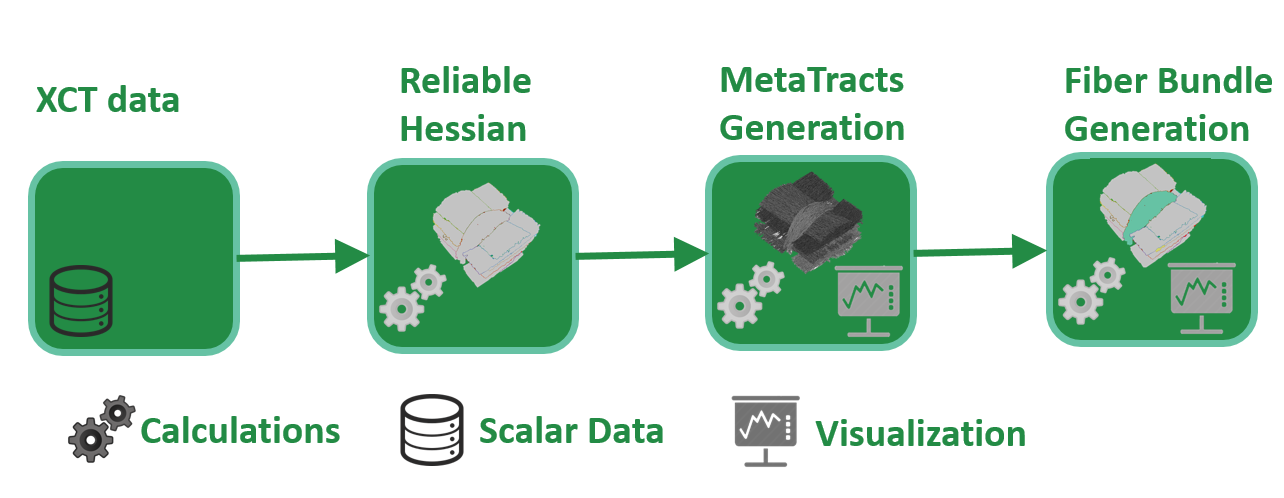
\includegraphics[width=0.45\textwidth]{imagesMT2014/algo.png}
	%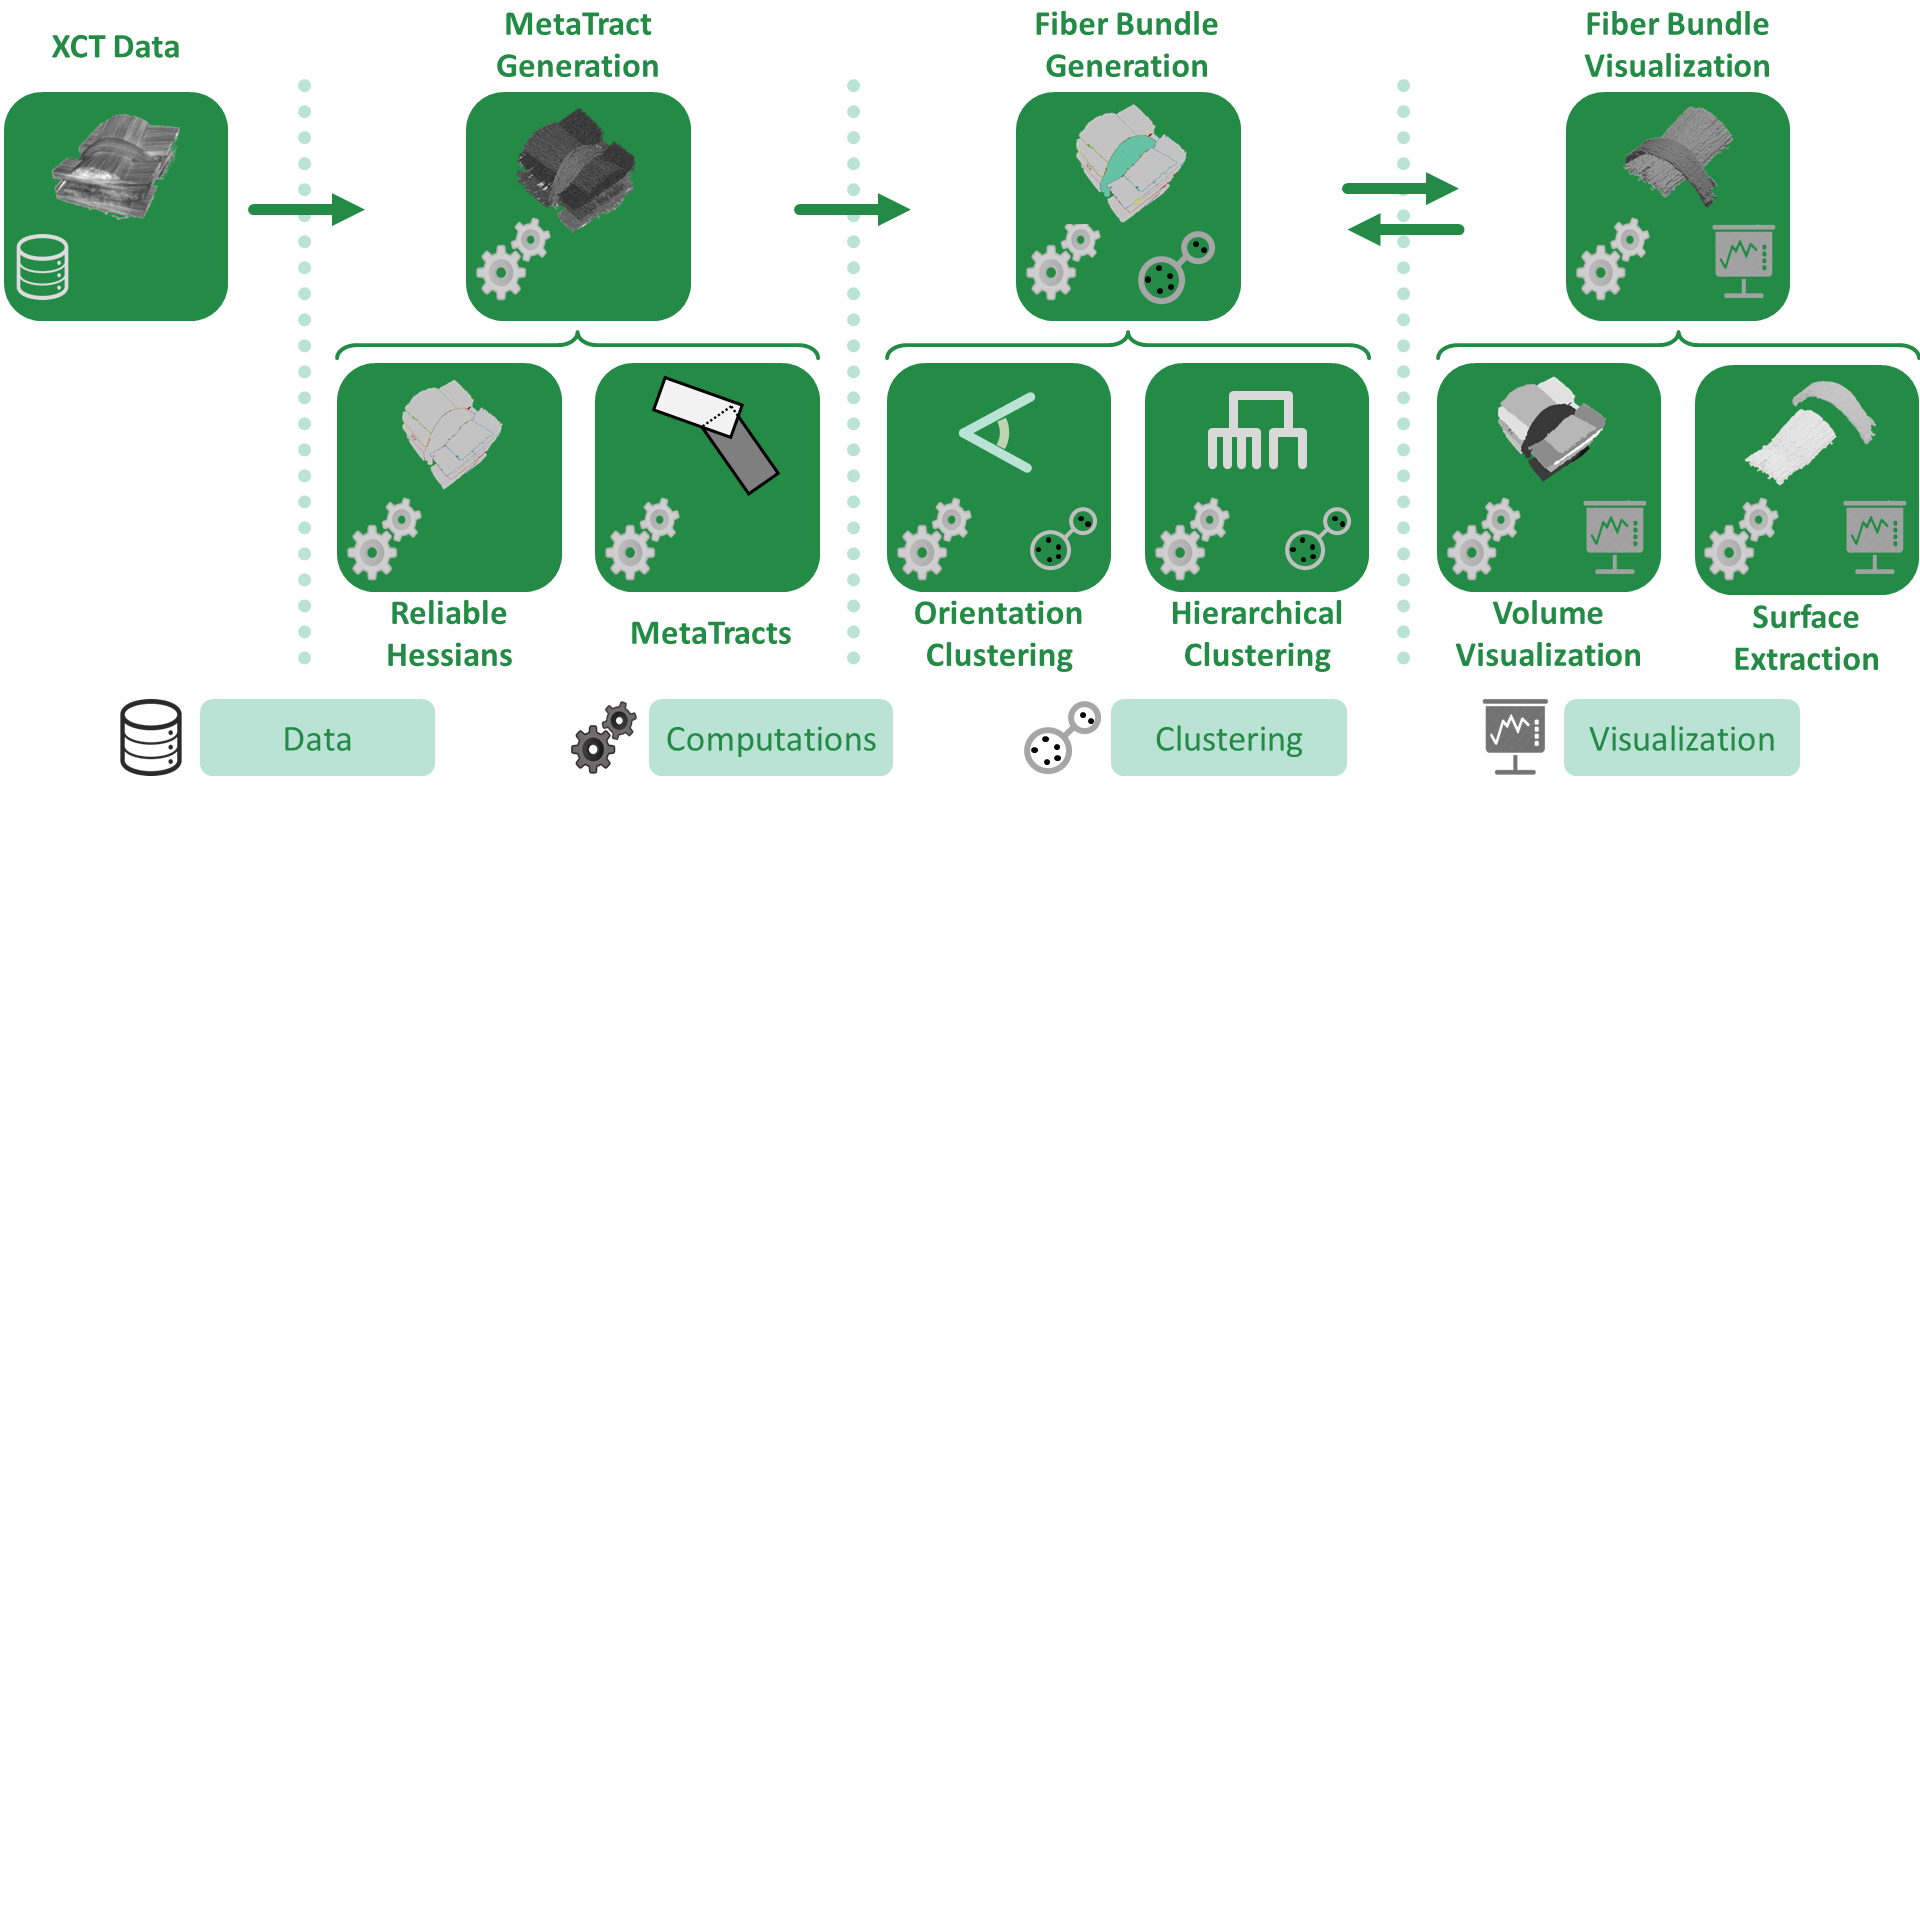
\includegraphics[width=0.5\textwidth,  trim = 0mm 300mm 0mm 0mm, clip,]{imagesMT2014/image_algo}
	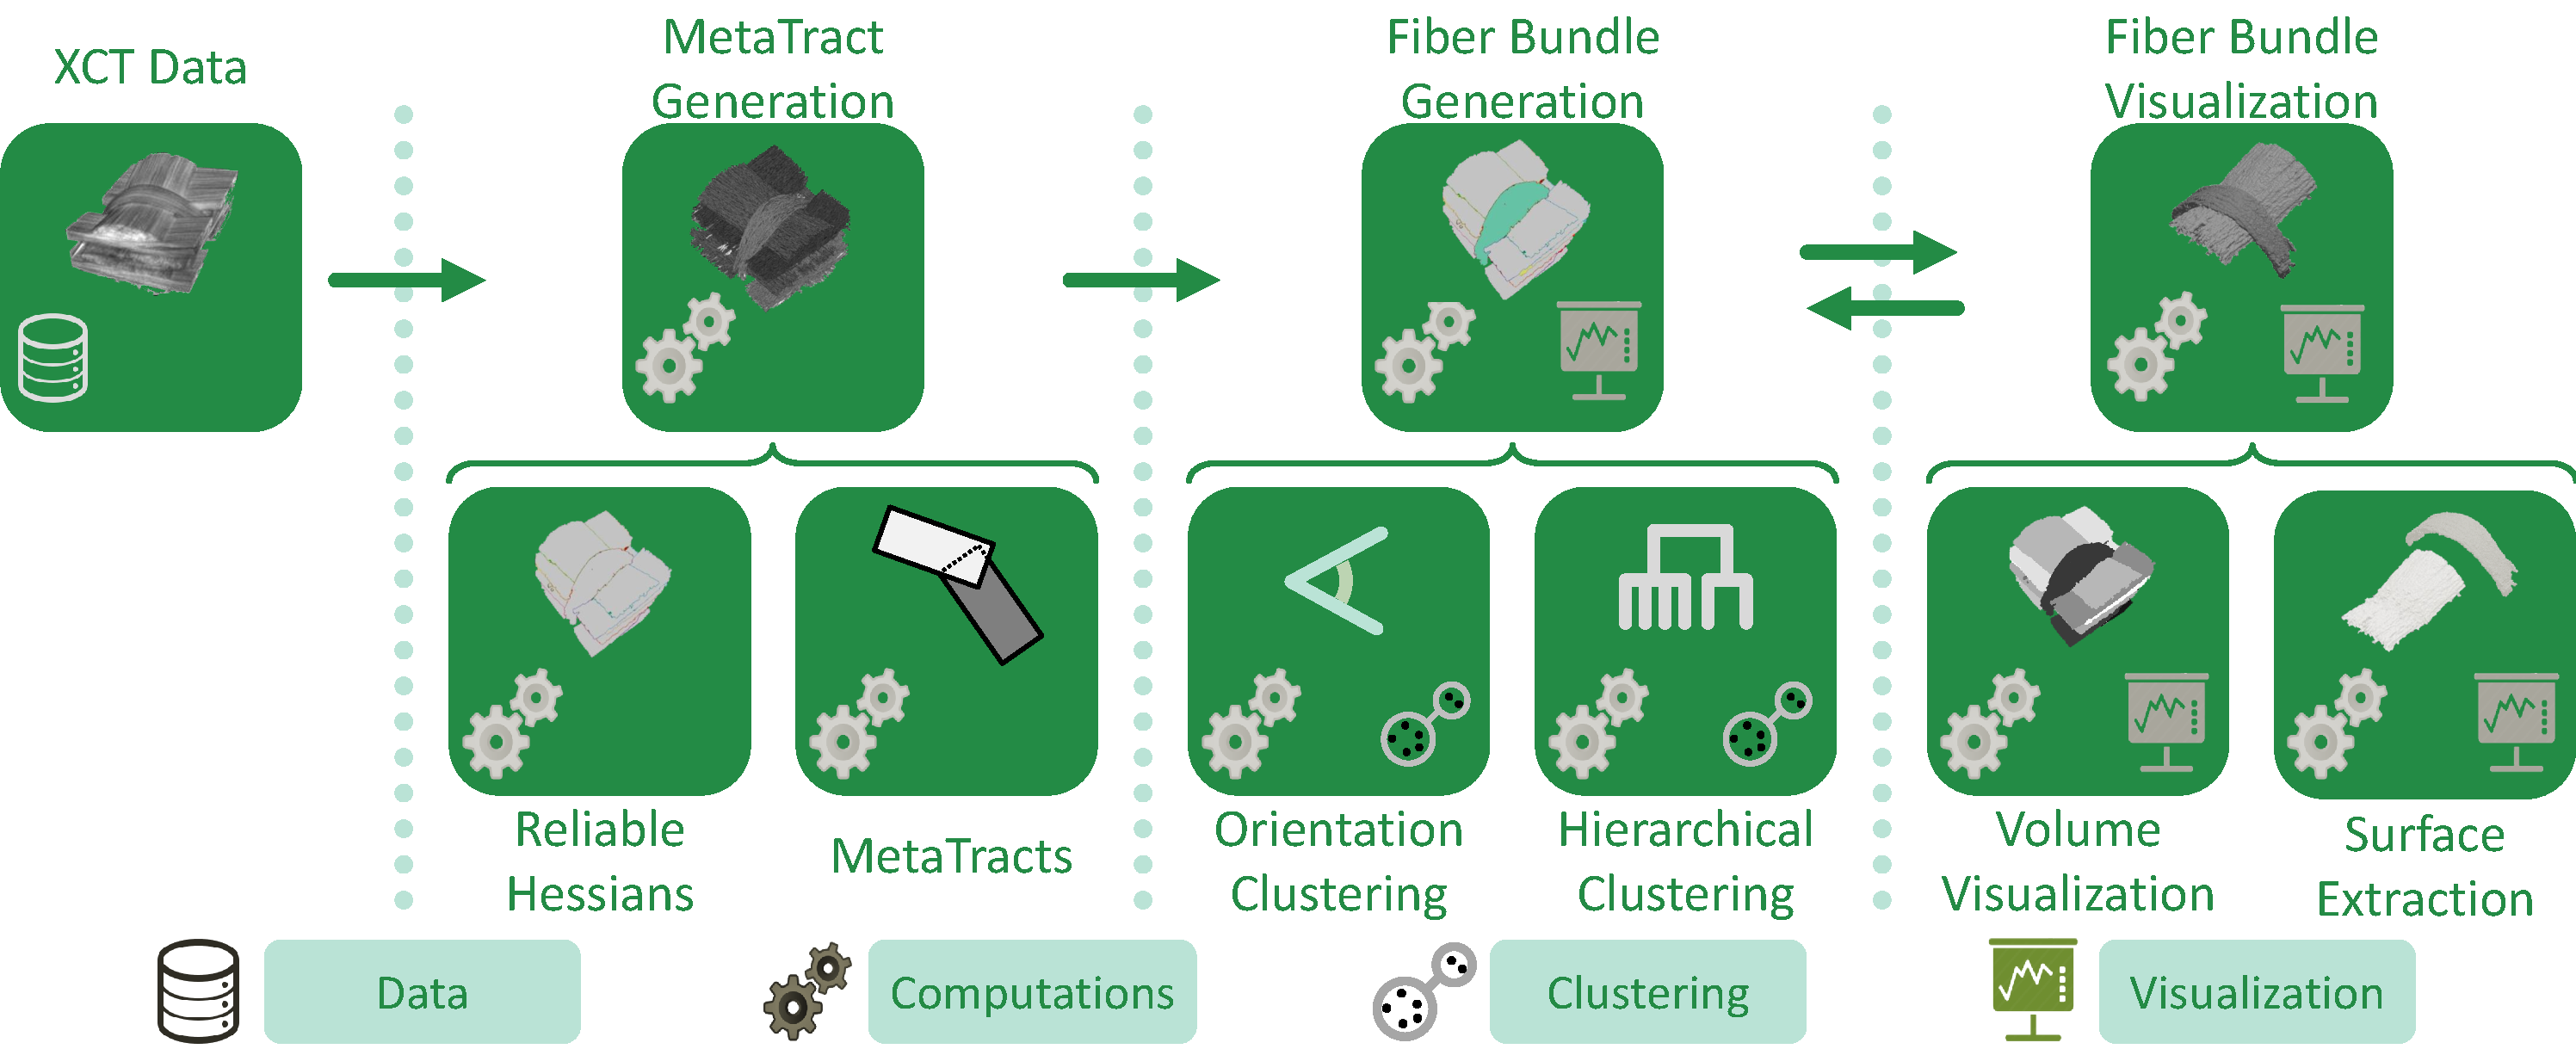
\includegraphics[width=\linewidth]{images_pvis/workflow.pdf}
	\caption{Flow chart of the MetaTracts approach for fiber bundle extraction}
	\label{fig:flowchart}
\end{figure}
Figure~\ref{fig:flowchart} shows an over view of our approach. Starting from XCT data, we first generate MetaTracts (see Sec.~\ref{sec:approach}). Then we cluster the MetaTracts to generate and visualize fiber bundles (see Sec.~\ref{subsec:fiber-bundles}). We discuss the visualizations we created for our domain experts in Sec.~\ref{sec:vis}. Sec.~\ref{sec:results} describes our experimental results, Sec.~\ref{sec:param_choices} presents our parameter choices and  Sec.~\ref{sec:user_eval} finally summarizes the user evaluation of our method.



\section {Related work}
\label{sec:prev_work}
%In order to analyze fiber bundles, whose individual fibers are barely visible, we studied a branch of visualization which seems to be completely off-topic at first sight: Diffusion Tensor Imaging (DTI). Tractography methods to reconstruct fibrous structures such as neural fibers in the human brain from magnetic resonance (MR) images has seen extensive research in recent years. Visualization techniques to reduce the geometric complexity and cluttering caused by dense fiber models of single fibers and emphasizing higher level structures called the fiber bundles have also gained popularity in recent years. In general these bundles are related anatomically or spatially.
%We broadly divide the related work on DTI  into two parts related to our method: fiber tracking and fiber clustering. Furthermore, methods analyzing second order local structure are considered as related work. Finally, we review the field of visual analysis of fiber reinforced composites in this section.

Diffusion Magnetic Resonance Imagining (dMRI, also referred to as Diffusion Tensor Imaging (DTI)) has gained popularity in medical diagnosis within recent years. Its main clinical application is found in the study and treatment of neurological disorders. DTI may reveal abnormalities in white matter fiber structure and is used for visualizing the organization of fibers in the human brain and brain connectivity.
A variety of algorithms have been proposed for generating fiber-tract trajectories. In general, these reconstructions of fiber trajectories are clustered in bundles which are expected to be related anatomically or spatially. 
We broadly divide the related work on DTI into two parts of immediate relevance to our proposed solution: fiber tracking and fiber clustering. We discuss methods for analyzing the second order local structure and review the current state of the art in the visual analysis of fiber reinforced composites.


\subsection {Fiber Tracking in Diffusion Tensor Imaging}
\label{subsec:fiberEx} 
A basic assumption in DTI analysis is that the principal eigenvector of the diffusion tensor is parallel to the underlying dominant fiber direction in each image voxel~\cite{Basser2002, Basser2000, Mori1999, Mori2002}. Continuous tracts are created by propagating virtual particles along fiber directions until they reach some termination criterion. 
This is usually done by solving a Runge-Kutta integration (typically second or fourth order). The principal diffusion direction at each discrete location is interpolated to form a continuous velocity field. 
Because decisions are made locally, these methods perform poorly in noisy regions and often generate small fibers. Basser et al.~\cite{Basser2002,Basser2000} proposed that white matter tracts could be represented as 3D curves in space. They showed that numerical methods could be used to follow fibers and fiber bundles and to generate tracts in human brain data. 
Mori et al.~\cite{Mori1999,Mori2002} divided reconstruction techniques into line-propagation or energy minimization techniques. In line propagation approaches, trajectories are computed based on local neighborhoods and in energy minimization approaches the most  favorable trajectory connecting two given endpoints is selected. 


\subsection {Fiber Clustering in Diffusion Tensor Imaging}
\label {subsec:fiberClus}
In DTI, a similarity measure based on factors such as proximity between fibers is used to group fiber tracts into bundles. Extensive research has been done on automatic DTI fiber clustering methods \cite{Brun2004,Brun2003,Corouge2004,westinMEDIA02,Zhang2008}. 
Clustering requires choosing a suitable proximity measure and a method for grouping ``close" fibers.
Pairwise proximity measures include endpoint distances~\cite{Brun2003} and mean of the closest distances between points on two fibers~\cite{Corouge2004}. Zhang et al.~\cite{Zhang2008} introduced a thresholded version of the of mean of closest distances, so that fibers which are close for certain distance and then diverge, are clustered separately. Brun et al.~\cite{Brun2004} use normalized cuts along with a pairwise distances measure computed using a 9D fiber shape descriptors. The choice of the clustering algorithm can be broadly divided into those approaches using hierarchical clustering~\cite{Moberts2005, Zhang2008} and those using spectral clustering~\cite{Brun2004,jonasson2005, ODonnell2007}.
Brun et al.~\cite{Brun2003} described how a spectral non-linear dimensionality reduction technique, Laplacian eigenmaps (Belkin and Niyogi~\cite{Belkin01}), can be applied to the problem of organizing fiber tracts data. The key notion of the Laplacian eigenmaps algorithm is to represent the underlying data as a graph. Each node represents a data point and the edges connect neighboring data points. An eigenvalue problem is solved to represent the data in a lower dimensional space while preserving the local graph structure. In the case of fiber bundles, the individual points are fiber tracts. In the ideal case fiber tracts belonging to the same bundle must remain ``close" to each other in the lower dimensional space. Westin et al.~\cite{westinMEDIA02} also use spectral clustering on a Hausdorff distance measure defined as the maximum of point wise minimum distances between two fibers. Jonasson et al.~\cite{jonasson2005} run k-means clustering on the eigenvectors of the affinity matrix defined as the co-occurrence of fibers in the data.
%The clustering methods have also been evaluated to be generally accurate in capturing fiber bundles as seen in Moberts et al.~\cite{Moberts2005} and Corouge et al.~\cite{Corouge2004}. 
The agglomerative hierarchical clustering method~\cite{DudaHartStork01} has gained popularity for proximity based fiber segregation (Zhang et al.~\cite{Zhang2008}, Corouge et al.~\cite{Corouge2004}). 
These approaches build on the assumption that proximity measures that compare DTI fiber trajectories can also represent anatomical relationships. An agglomerative hierarchical clustering method starts with each data point/fiber in an individual cluster. At each stage of the algorithm the two most similar clusters are merged based on some criterion. The two basic cluster similarity measures are single-link and complete-link. With the single link measure the distance between the clusters is the distance between the closest pair of items. 
Moberts et al.~\cite{Moberts2005} implemented several distance measures in their evaluation of fiber clustering and concluded that clustering methods are generally accurate in capturing fiber bundles. 
%Mean of closest distances performs better than closest point distance computations or Hausdorff distance measures and hierarchical clustering using single-link measure gave the best results. 
There are a number of difficulties in hierarchical clustering. First, computing all pairs' distances for tracts to generate the distance matrix is time consuming~\cite{Garyfallidis2012}. Second, a ``correct'' distance measure to compare tracts must be chosen. Third, hierarchical clustering is best suited for similar length fibers.
Spectral methods are also hindered by long matrix computations.


\subsection{Second order local structure}
Unlike DTI, we do not have diffusion tensor data. Instead, we have a scalar volume with tubular structures embedded in them. Analyzing curvilinear structures in volumetric images has been utilized for a variety of purposes including center line extraction~\cite{Bouix2005} and vascular image enhancement as proposed by Frangi et al.~\cite{Frangi1998} and Sato et al.~\cite{Sato1997}. Frangi et al.~\cite{Frangi1998} introduced a method based on studying the eigenvalues of the Hessian matrix specifically for the purposes of developing vessel enhancement filters.


\subsection {Visual Analysis and Modeling of Fiber Reinforced Composites}
The approaches presented in visualization and analysis of composites mainly focus on individual objects such as fibers or pores and deals with fiber extraction from high resolution data where the individual fibers are clearly discernible. Fritz et al.~\cite{Fritz2009} proposed workflows for NDT practitioners to explore and quantify steel fibers in reinforced sprayed concrete. This approach allows analyzing fiber orientations based on direction transfer functions. Salaberger et al.~\cite{Salaberger2011} introduced a pipeline to extract and characterize individual fibers of fiber reinforced composites. They encode the extracted fibers as color-coded line segments in 3D and visually identifying fibers with similar orientations. Recently, Weissenbock et al.~\cite{Weissenbock2014} introduced a system for interactive exploration and analysis of fibers in fiber reinforced polymers. 
Lomov et al.~\cite{Lomov2010, Lomov2001} and Straumit et al.~\cite{Straumit2014}, discussed problems and current available solutions in geometric modeling of three dimensional composites. Modeling of the composites, first starts with establishing the topology of the structure, which translates to answering if a particular bundle is in contact with another at a particular position. The second step builds the geometry of the model, answering questions relating to placement of bundles in space their orientations and dimensions. 
%Tools based on image analysis, fiber tracking and clustering into bundles in DTI and their subsequent visualization through stream tubes and coloring schemes have received extensive research. Recently, similar techniques have been applied to fiber tracing in composite materials. 
To the best of our knowledge there is no approach focusing on direct extraction of fiber bundle structures from low resolution XCT of CFRP laminates.

%To the best of our knowledge there is no approach focusing extraction of fiber bundles structures of low resolution XCT  of composite fibers, which is the main scope of this work.

%\begin{figure}
%  \begin{center}
%    \includegraphics[width=0.25\textwidth,clip=true, trim=2cm 2cm 0cm 2cm]{imagesMetaTracts/crop-13-total}
%  \end{center}
% \caption{Volume rendering of a part of a dataset. Fig.~\ref{fig:slice_data:a} and ~\ref{fig:slice_data:b} show image slices along the blue and red plane respectively. }
% \label{fig:orig_data}
%\end{figure}
%\begin{figure}[h]
%  \centering
%              \subfloat [][A single slice along blue plane in fig~\ref{fig:orig_data}.]
%                        {\includegraphics[width=0.22\textwidth]{imagesMetaTracts/crop-13-1c-anno.png}\label{fig:slice_data:a}}\quad 
%                        \subfloat [][A single slice along the red plane in fig~\ref{fig:orig_data}]
%                        {\includegraphics[width=0.22\textwidth]{{imagesMetaTracts/crop-13-1b-anno}}\label{fig:slice_data:b}}
%  \caption{Single slices along different orientations of the data set. In Fig.~\ref{fig:slice_data:b}, the red annotation demarcates the boundary between two different bundles. The green squares show that the cross sections of the bundles also widely vary.}
%  \label{fig:slice_data}
%\end{figure}

\begin{figure}[tb]
\centering
%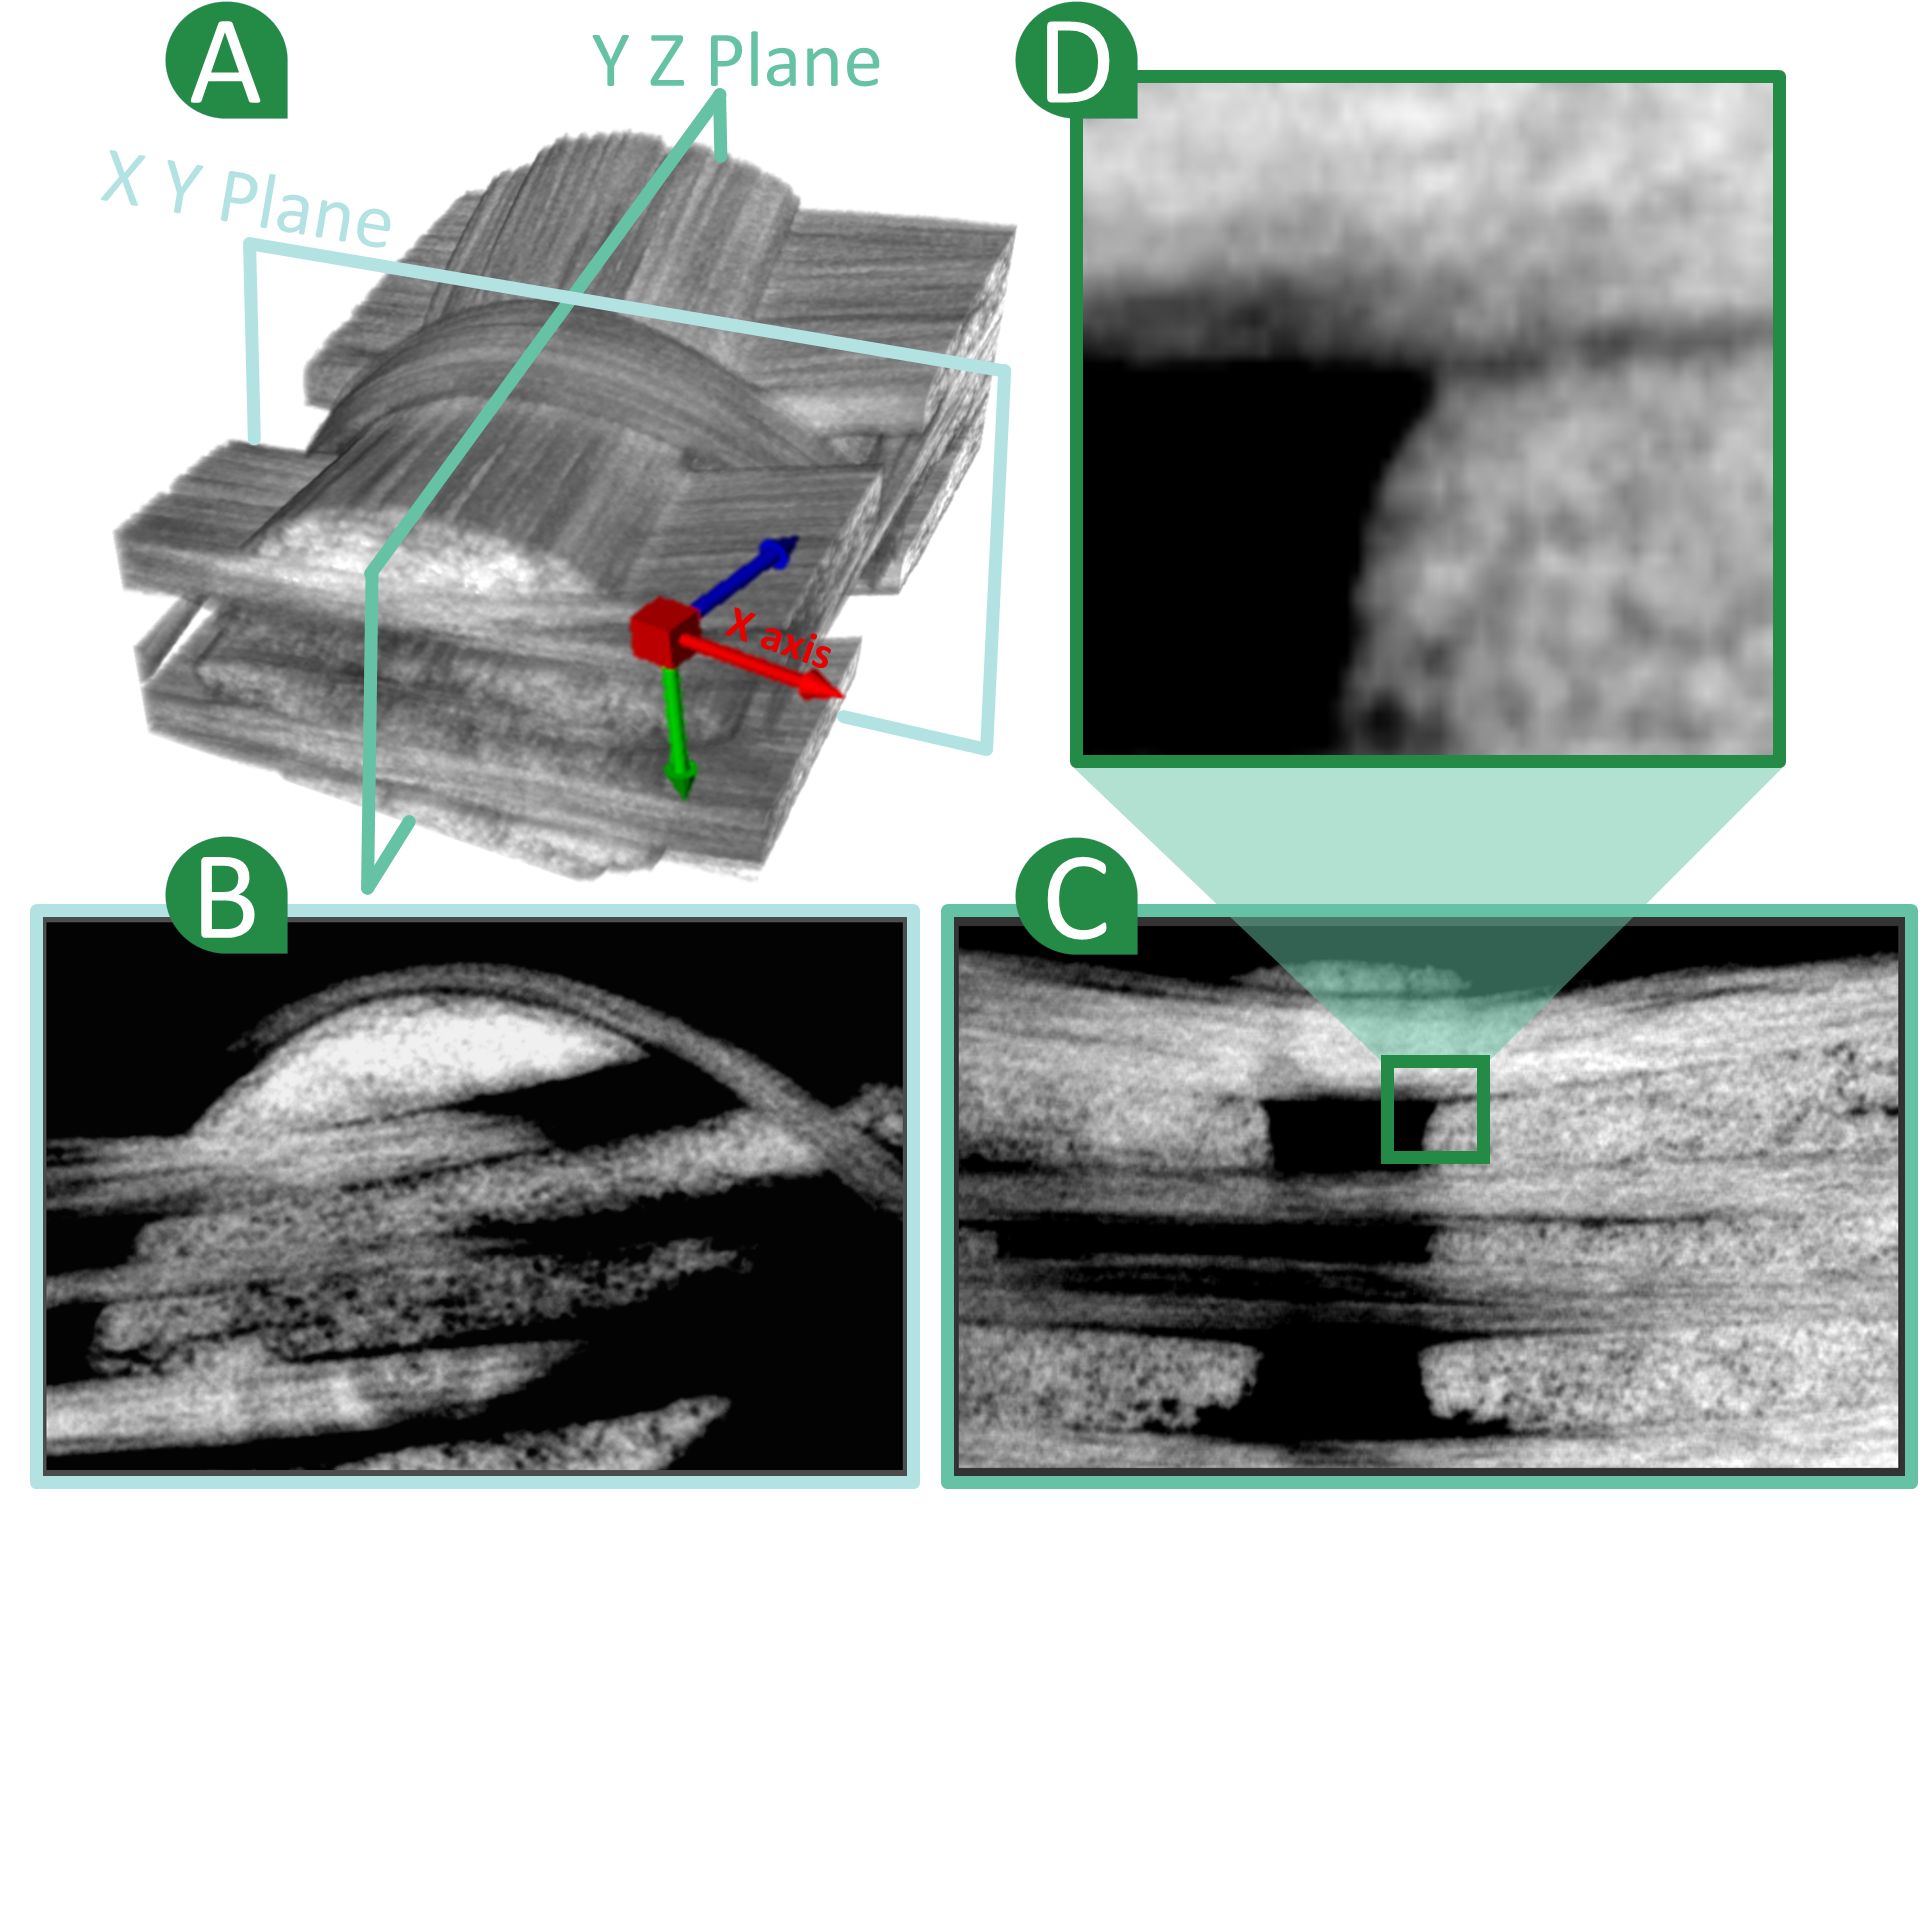
\includegraphics[width=0.5\textwidth, trim = 0mm 110mm 0mm 0mm, clip,]{images_pvis/figure1}
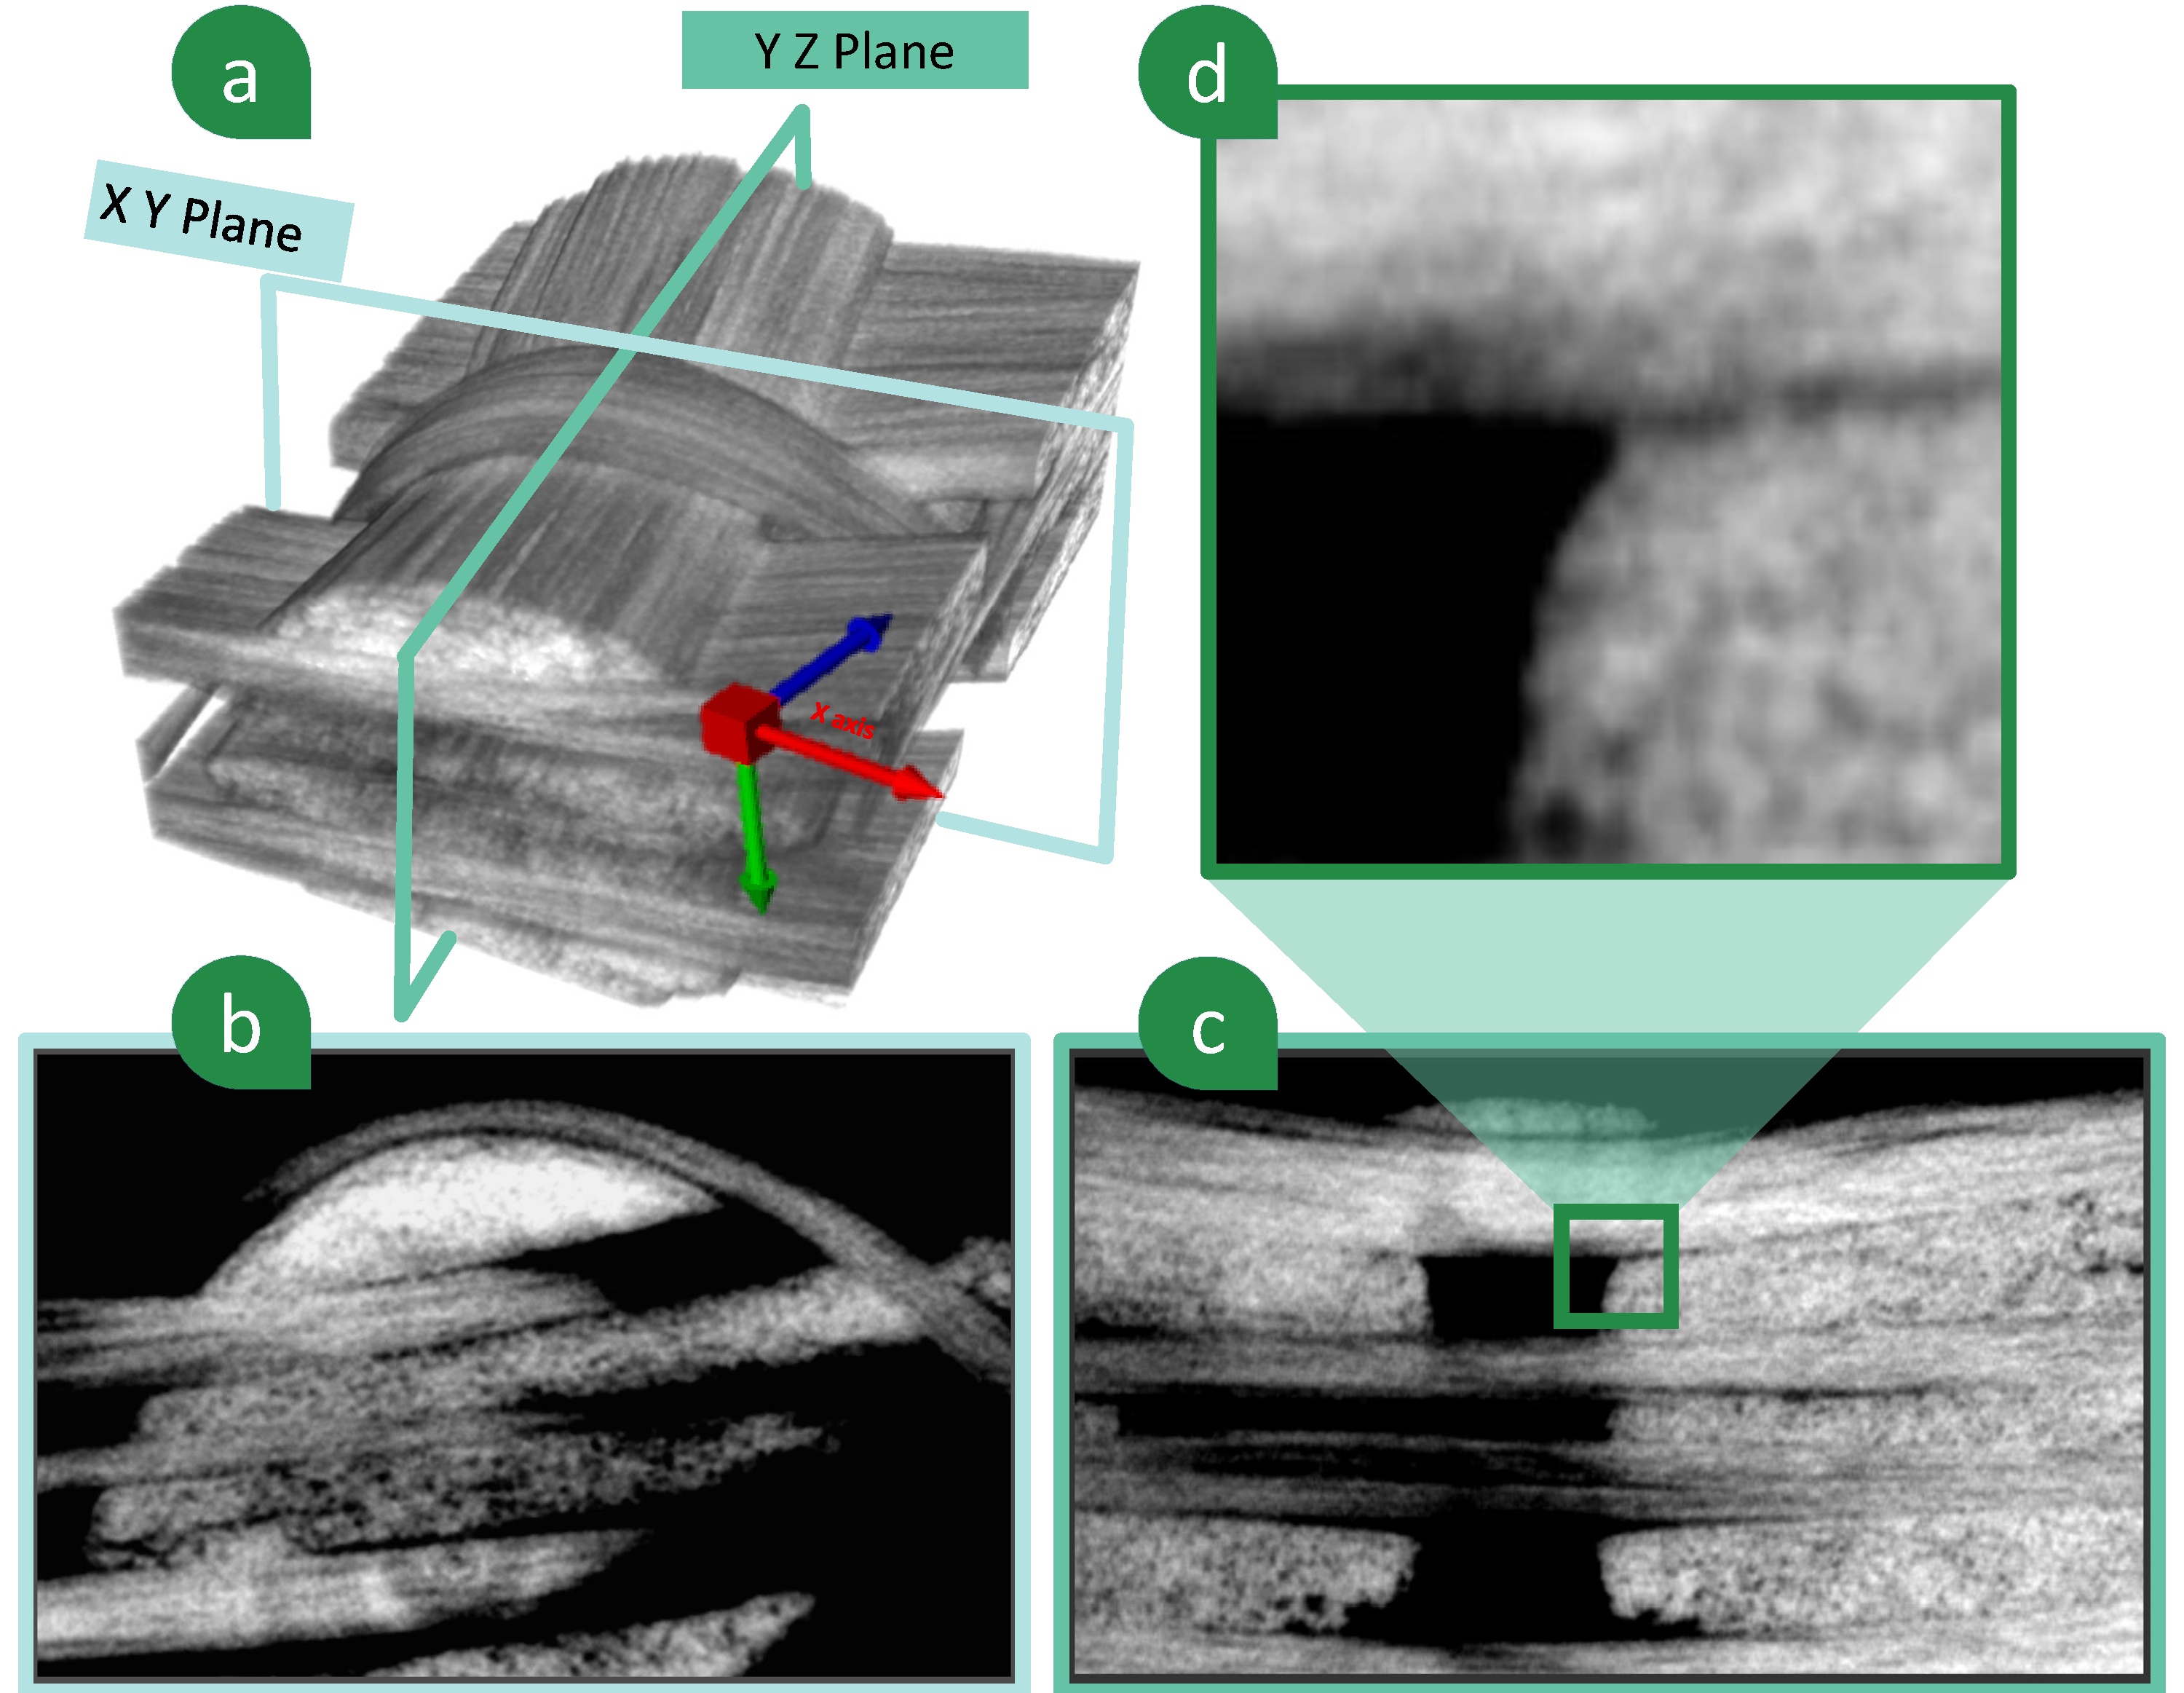
\includegraphics[width=\linewidth]{images_pvis/data-char.pdf}
\caption{Data characteristics: (a) Rendering of dataset D1. (b, c) 2D slices along Z- and X-axis. (d) Zoom in of the green region marked in (c). Multiple fiber bundles cross and are indistinguishable by visual inspection alone. }
\label{fig:data-char}
\end{figure}


\section {Data Characteristic and Assumptions}
\label{sec:char_data}
Figure~\ref{fig:data-char} shows dataset D1 with woven fiber bundles. The size of D1 is 450$\times$300$\times$500 voxels with isotropic resolution of 2 $\mu m$ and 8 bit unsigned integer scalars. Figure~\ref{fig:data-char} clearly shows the recurring fiber bundle weaving pattern of the composite unit cell used for manufacturing. Figure~\ref{fig:data-char}a shows a volume rendering of the dataset. Figure~\ref{fig:data-char}b and ~\ref{fig:data-char}c show 2D slices along the $X$- and the $Z$-axis respectively. Figure~\ref{fig:data-char}d zooms into the green region of interest. 
The resolution of D1 renders the individual carbon fibers in a fiber bundle hard to resolve in the 2D slice images. Figure~\ref{fig:data-char}d contains two bundles going in opposite directions. Also the separation between two fiber bundles is barely visible. The fiber bundles may differ in terms of the amount of fibers in the bundle. Figure~\ref{fig:data-char}a shows the large variation in cross section sizes among the bundles.
Depending on the weaving pattern, the fiber bundles cross each other in different orientations. The number of orientations is defined by the weaving pattern and typically consists of two main orientations. The weaving pattern may cause individual bundles to be curved. In consequence, individual fibers may be adjacent in Euclidean distance but belong to different bundles. 
We make the following \textit{assumptions} on our data:

\begin{itemize}[noitemsep]
\item The structure embedded in the data contains fiber bundles of indiscernible fibers.
\item Local orientation: each point in a fiber bundle has a local orientation parallel to the corresponding area in the fiber bundle.
\item Local orientation may gradually change in the fiber bundle.
\item Local orientation may be noisy and not reliable.
\item Connectivity: moving along the direction of a non-noisy local orientation in small increments, we will reach another neighborhood with similar local orientation.
\item Fiber bundles going in different directions only interact near the surface of contact.
\end{itemize}
%\begin{figure}[htp]
%  \centering
%    \subfloat[Overview of the dataset]{\label{figur:3}\includegraphics[scale=0.3]{imagesMetaTracts/crop13-a.eps}}
%  \subfloat[X Axis]{\includegraphics[width=40mm, height=40mm]{imagesMetaTracts/xaxis.eps}}\label{figur:1}\\
%  \subfloat[Y Axis]{\label{figur:2}\includegraphics[width=40mm, height=40mm]{imagesMetaTracts/yaxis.eps}}
%  \subfloat[Z Axis]{\label{figur:3}\includegraphics[width=40mm, height=40mm]{imagesMetaTracts/zaxis.eps}}
%  \caption{One of our datasets.Fig \ref{fig:orig_data}(a) provides an overview of the entire volume, the rest show slices of each of the major axis.}\label{fig:orig_data}
%\end{figure}

%\begin{figure}[b]
%\centering
%\includegraphics[width=\linewidth]{imagesMetaTracts/crop-13-3.eps}
%\caption{Volume rendering of the scalar volume of one of our data set. Cut-out A shows a slice along the X axis, cut-out B shows a slice along the Z axis.}\label{fig:orig_data}
%\end{figure}


\section {Extracting MetaTracts }
\label{sec:approach}
Extracting the MetaTracts consists of two  major steps. First, we extract a local orientation vector at each grid location (Sec.~\ref{subsec:rh}). Second, we compute coarse poly-cylinders called MetaTracts which traverse the data (Sec.~\ref{subsec:mtprop}).

%\subsection {Extracting MetaTracts}
%\label{subsec:ExFiberCyl}
%We explain the different steps of MetaTracts extraction.


\subsection {Reliable Hessians}
\label{subsec:rh}

The input to the first stage of our pipeline is the original scalar dataset in a uniform lattice grid in $\mathbb{R}^3$. As output, each grid location gets associated with an unit vector representing the local orientation and a real value [0,1] representing a measure of the reliability of the local orientation. We approximate the local orientation by eigenvalue analysis of the Hessian matrix computed at each voxel.
The Hessian matrix represents the local curvature. The eigen decomposition of the Hessian matrix gives the eigenvectors which describe the local second-order structure of the image.
The eigenvector corresponding to the smallest eigenvalue (also referred as the principal direction) gives the direction along which the curvature is smallest. This direction coincides with the direction of the tubular structure.

Frangi et al.~\cite{Frangi1998} introduced a process that searches for geometric structures which are tubular. They define a measure based on two geometric ratios of the second order ellipsoid given by the local Hessian matrix to measure the \textit{vesselness} criterion. In order to determine \textit{reliable Hessians} for our approach, we make use of the vesselness criterion as follows: Let $\lambda_{K}$ be the eigenvalue with the $K^{th}$ smallest magnitude. Here, $|{\lambda}_{1}| \leq| {\lambda}_{2}|\leq| {\lambda}_{3}| $ are the eigenvalues of the Hessian matrix. Specifically, a pixel belonging to a vessel region will have small $\lambda_{1}$ ($|\lambda_{1}|\approx 0$) and $\lambda_{2}$, $\lambda_{3}$ of large magnitude and of equal sign($|\lambda_{1}| \ll |\lambda_{2}|$ and $|\lambda_{2}|\approx |\lambda_{3}|$). The sign indicates if the vessel is bright in a dark background or dark in a bright background. In our case the individual fibers are bright ($\lambda_2,\lambda_3 < 0$). The following measures are defined in~\cite{Frangi1998}.  

\begin{equation}\label{RA}
\mathcal{R_{A}}=\frac{\textrm{Largest  Cross Section}\big/ \pi}{{\textrm{Largest Axis Semi-length}}^{2}}=\frac{|\lambda_{2}|}{|\lambda_{3}|}
\end{equation}

\begin{equation}\label{RB}
\mathcal{R_{B}}=\frac{\textrm{Volume}\big/ (4\pi \big/ 3)}{{(\textrm{Largest Cross Section Area}\big/ \pi)}^{\frac{3}{2}}}=\frac{|\lambda_{1}|}{\sqrt{|\lambda_{2}\lambda_{3}|}}
\end{equation}
In Equation~\ref{RB}, $\mathcal{R_{B}}$ provides a measure of deviation from a blob like structure while in Equation~\ref{RA}, $\mathcal{R_{A}}$ distinguishes between plate-like and line-like structure. Grey-scale variations and close proximity of the fibers in our data make the Hessians computed at each voxels susceptible to errors. Thus, we compute reliable Hessians ($R_H$) to determine which locations in the volume provide reliable local orientation. 
%($R_H$ is similar to the vesselness in~\cite{Frangi1998}).
%Thus, we compute the ``vesselness'' measure to determine which locations in the volume provide reliable local orientation.
$$
R_{H} = \left\{ \begin{array}{ccc}
 0 & \mbox{ if $\lambda_{2}>0$ or $\lambda_{3}>0$} \\
  (1-e^{\frac{\mathcal{-R_{A}}^{2}}{2\alpha^{2}}})
  (e^{\frac{\mathcal{-R_{B}}^{2}}{2\beta^{2}}}) (1-e^{\frac{-s^2}{2c^2}}) &\mbox{ otherwise}
       \end{array} \right.
$$
Variable $s$ is the Frobenius norm of the Hessian matrix. The value of $(1-e^{\frac{-s^2}{2c^2}})$ will be low in regions with no structure. The utility of the vesselness is a little different in our framework than Frangi et al.~\cite{Frangi1998}.
First, vesselness in biology is computed for different scales because the vessels can be of different sizes. In our case, usually the width of individual fibers are known a priori.
Second, and more importantly, we do not have clear tubular structures embedded in a dark contrast matrix such as in blood vessels.
Instead, we are trying to associate each grid location  with a probable orientation based on its local second order structure. The $R_{H}$ is interpreted as a reliability measure of the local orientation.
Grid locations where the $R_{H}$ is above a cutoff threshold are marked as regions with reliable orientations (see Sec.~\ref{sec:param_choices} on parameter choices).
%\begin{figure}[h]
%	\centering
% \subfloat[]{ \includegraphics[width=0.2\textwidth,clip=true,trim=0cm 1cm 0cm 1cm]{imagesMetaTracts/crop-13-tracks-hess.eps}\label{fig:r_h:a}}
%   \subfloat[]{\includegraphics[width=0.25\textwidth,scale=0.2]{imagesMetaTracts/rh-1c-anno.png}\label{fig:r_h:b}}
%  \caption{Reliable Hessians: (a) Shows $R_{H}$ colored according to the absolute value of the normalized major eigenvector (local orientation) mapped to RGB color space. Fig~\ref{fig:r_h:b} shows part of a single slice where two bundles along Z(blue)axis and X(red)axis meet. Spurious specks shows that the local orientation is still noisy. Black denotes area below the $R_H$ threshold.}\label{fig:r_h}
%\end{figure}
%\begin{figure}
%\centering
%\includegraphics[width=0.4\textwidth,scale=0.1,clip=true,trim=0cm 1cm 0cm 1cm]{imagesMetaTracts/crop-13-hess-2}
% \caption{Reliable Hessians: Left, shows $R_{H}$ colored according to the absolute value of the normalized major eigenvector (local orientation) mapped to RGB color space. Right, shows a single slice along the X axis. Spurious specks shows that the local orientation is still noisy. Black denotes area below the $R_H$ threshold.}\label{fig:r_h}
%\end{figure}
In Figure~\ref{fig:reliable_hessian} we see the intermediate results of the local orientation computation only at locations where $R_{H}$ is greater than the cutoff threshold. The unit vector representing the principal direction has been mapped to RGB color space. 
%Figure~\ref{fig:reliable_hessian}a shows the entire data set. 
Regions where the principal direction is parallel to the X axis are red in color, directions parallel to Y are green and those parallel to the Z are blue. Figure~\ref{fig:reliable_hessian}b and c show 2D slices along the Z and X axes respectively. Figure~\ref{fig:reliable_hessian}d shows a magnified region of interest. Note, the dark regions within a bundles are regions where the $R_H$ is less than the threshold and therefore considered as unreliable. The bundles are not uniformly colored, the Hessians and the corresponding directions are noisy.
% We note some intrinsic differences between the DTI and our XCT data. The Hessian computation works best when the tubular structures are well separated from the surrounding, unfortunately, this is not the case for our data (Fig.~\ref{fig:r_h}). Thus the local orientation at each voxel for XCT data is inherently more noisy (Fig.~\ref{fig:r_h} Right) than those computed from eigen analysis of diffusion tensors in DTI datasets.
We also note here some intrinsic differences between the DTI and our XCT data. Fiber traces can be created in DTI using a standard fiber tracking algorithm following the principal direction of diffusion using a fourth order Runge-Kutta method~\cite{Brun2003}. The principal direction based on the Hessian matrix works best when the tubular structures are well separated from the surrounding. This is not the case for our data. The local orientation at each voxel is inherently more noisy.

\begin{figure}[tb]
\centering
%\includegraphics[width=0.45\textwidth]{images_pvis/figure3}
%\includegraphics[width=0.5\textwidth,  trim = 0mm 90mm 0mm 0mm, clip]{images_pvis/figure3}
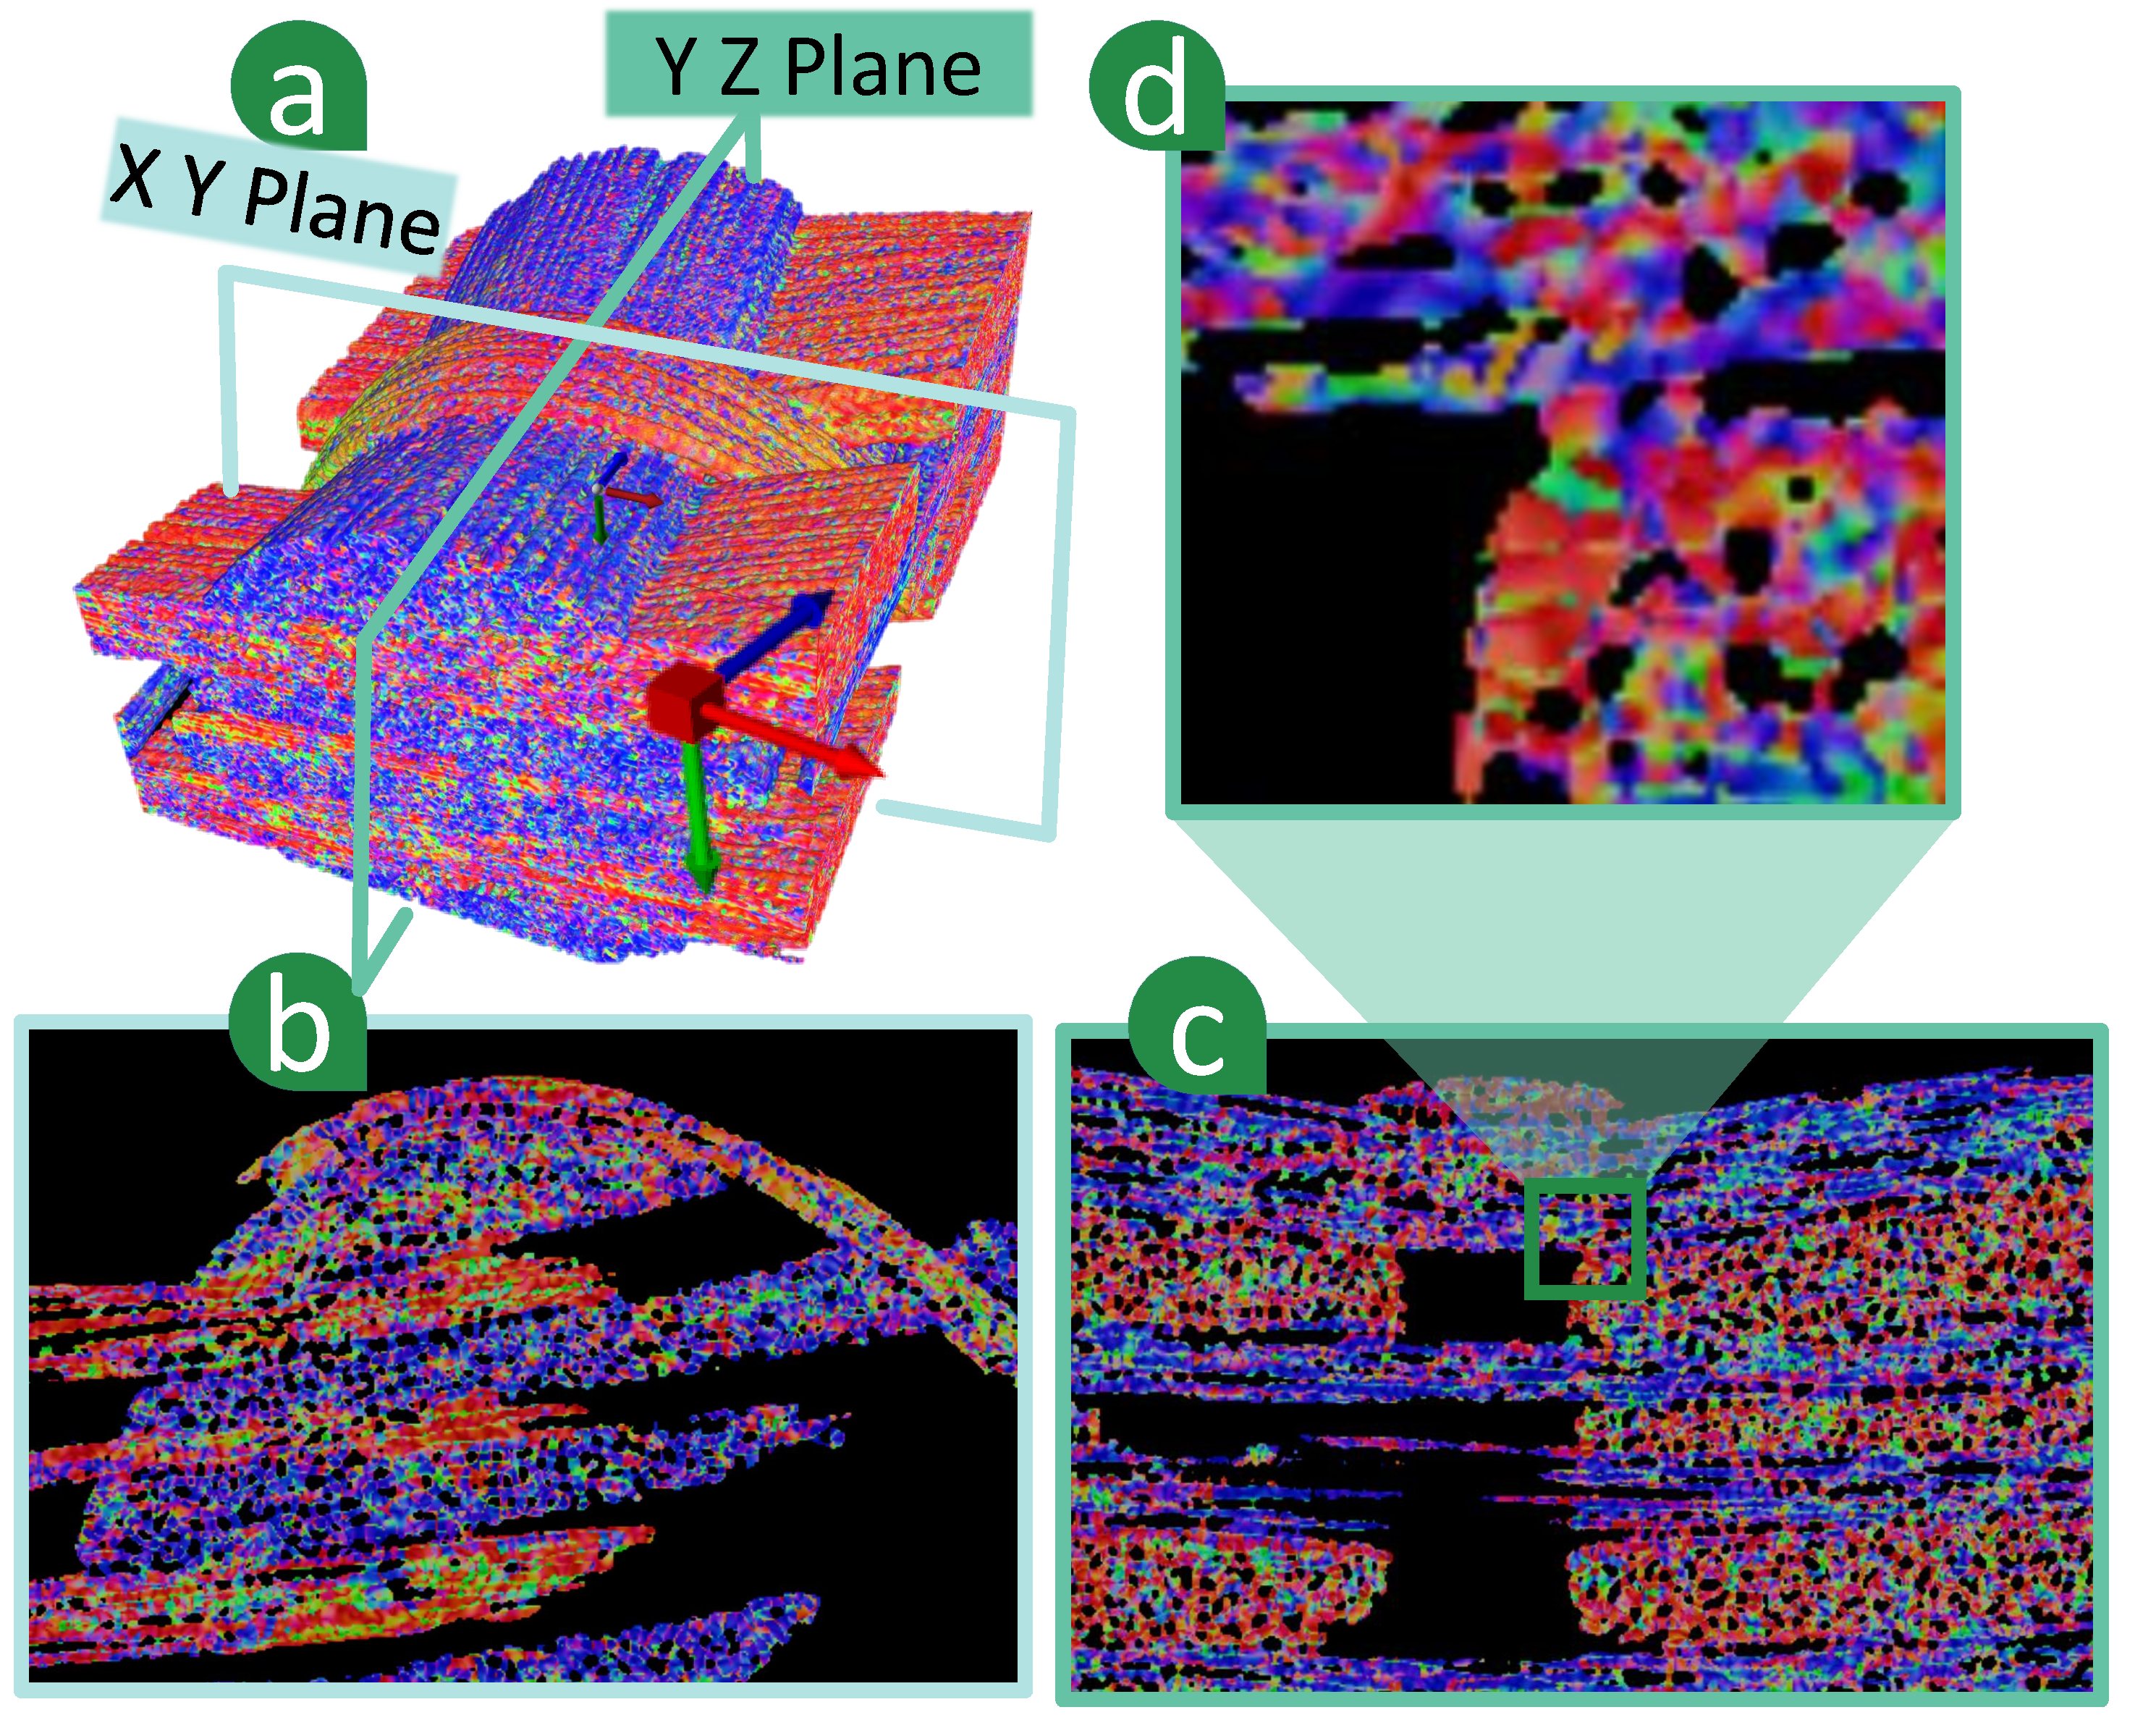
\includegraphics[width=\linewidth]{images_pvis/reliable_hessian.pdf}
 \vspace{-1.5em}
\caption{Reliable Hessians. (a) Colored according to Orientation vector mapped to RGB. (b,c) 2D slices along Z- and X axis. (d) Zoom in of the green region marked in (c).}
\label{fig:reliable_hessian}
\end{figure}


\subsection {MetaTracts properties and description} 
\label{subsec:mtprop}
%\begin{figure*}
%  \centering
%  \subfloat[Meta tract generation in 2D]{\includegraphics[width=0.5\linewidth]{imagesMetaTracts/algo-1b.eps}}
%  \subfloat[Orientation based similarity measure]{\includegraphics[width=0.5\linewidth]{imagesMetaTracts/algo-1c.eps}}
%  \caption{Simplified examples of meta tract generation process and orientation based similarity measure}
%  \label{fig:algo}
%\end{figure*}
%\begin{figure*}
%  \centering
%  \subfloat[]{\includegraphics[width=0.2\textwidth]{imagesMetaTracts/algo-1d}}
%  %\subfloat[Orientation based similarity measure]{\includegraphics[width=0.5\linewidth]{imagesMetaTracts/algo-1c.eps}}
%  \caption{Simplified example of meta tract generation process.}
%  \label{fig:algo}
%\end{figure*}
The input to this step is a grid in $\mathbb{R}^3$ where each grid point is associated with a normalized local orientation and a corresponding $R_H$ value.
Traditional integral curve based techniques cannot be used to extract fiber bundle traces from the reliable Hessians because of the spurious nature of the Hessian based local orientation. Thus instead of building fiber traces, we wish to find an abstract representation of the fibers. We build on the key assumptions on the data, namely ``local orientation" and ``connectivity" while taking into account the noise and lack of resolution. We do this by interpreting the underlying geometric structure of the fibers as a set of cylinders.
MetaTacts are a coarse and simple approximation of integral curves in the form of a continuous chain of cylindrical tubes in $\mathbb{R}^3$ traversing the fiber bundles embedded in the input data. MetaTracts share the following \textit{properties}:

\begin{enumerate}[noitemsep]
\item{MetaTract are associated with a continuous set of cylinders.}
\item{MetaTract are associated with a start point at a grid vertex.}
\item{Individual cylinders in a MetaTract have a constant length, a constant radius and a start point (which is also a grid vertex).}
\item{Individual cylinders in a MetaTract (except the first one) are connected to their previous cylinders at their start point.}
\item{Individual cylinders are parallel to the local orientation at their start points.}
\end{enumerate}


% $N_{p}$ (Fig.~\ref{fig:algo} provides an overview). Let $C_{p}$ be the grid point associated with the current cylinder. We insert a subset of the grid points $G_{q}$ that lie within the cylinder into a priority queue. The priority is defined by equation \ref{eqn:algo_1}. In Equation \ref{eqn:algo_1}, $angle$ refers to the angle between the local orientation at the current point $C_{p}$ and the grid point $G_{q}$. $PerpDist$ refers to the perpendicular distance between the $G_{q}$ and $C_{p}$ projected along the direction of the local orientation $N_{p}$. We only insert a grid point $G_{q}$ in the priority queue if the $angle$ is less than 20 degrees and the $PerpDist$ is at least 0.5. This ensures that points with obvious spurious local orientation or points which are very close to  $C_{p}$ are not put in to the queue. This simple check ensures our memory requirements are not excessive.


\subsection {MetaTracts generation}
\label{subsec:MetaTracts-generation}
In this section we explain the process of MetaTracts generation in $\mathbb{R}^2$ (the procedure trivially extends to $\mathbb{R}^3$). In $\mathbb{R}^2$, all the above properties hold except that cylinders are replaced by rectangles. The reliable Hessian step generates a local orientation vector in $\mathbb{R}^2$ and a reliability measure $R_H$[0,1]. In Figure~\ref{fig:algo}, regions with unreliable Hessian have been marked in blue. Figure~\ref{fig:algo}c shows an individual cylinder of a MetaTract. Let the seed point associated with the MetaTract be grid point $C_{p}$ (property 2 in Sec.~\ref{subsec:mtprop}). The local orientation at $C_p$ as computed in the step above is $N_P$ and is given by the dark green arrow. We generate a rectangle of length $L$ and radius $R$ (properties 3 and 5 in Section~\ref{subsec:mtprop}). 
%
\begin{figure}[tb]
  \begin{center}
 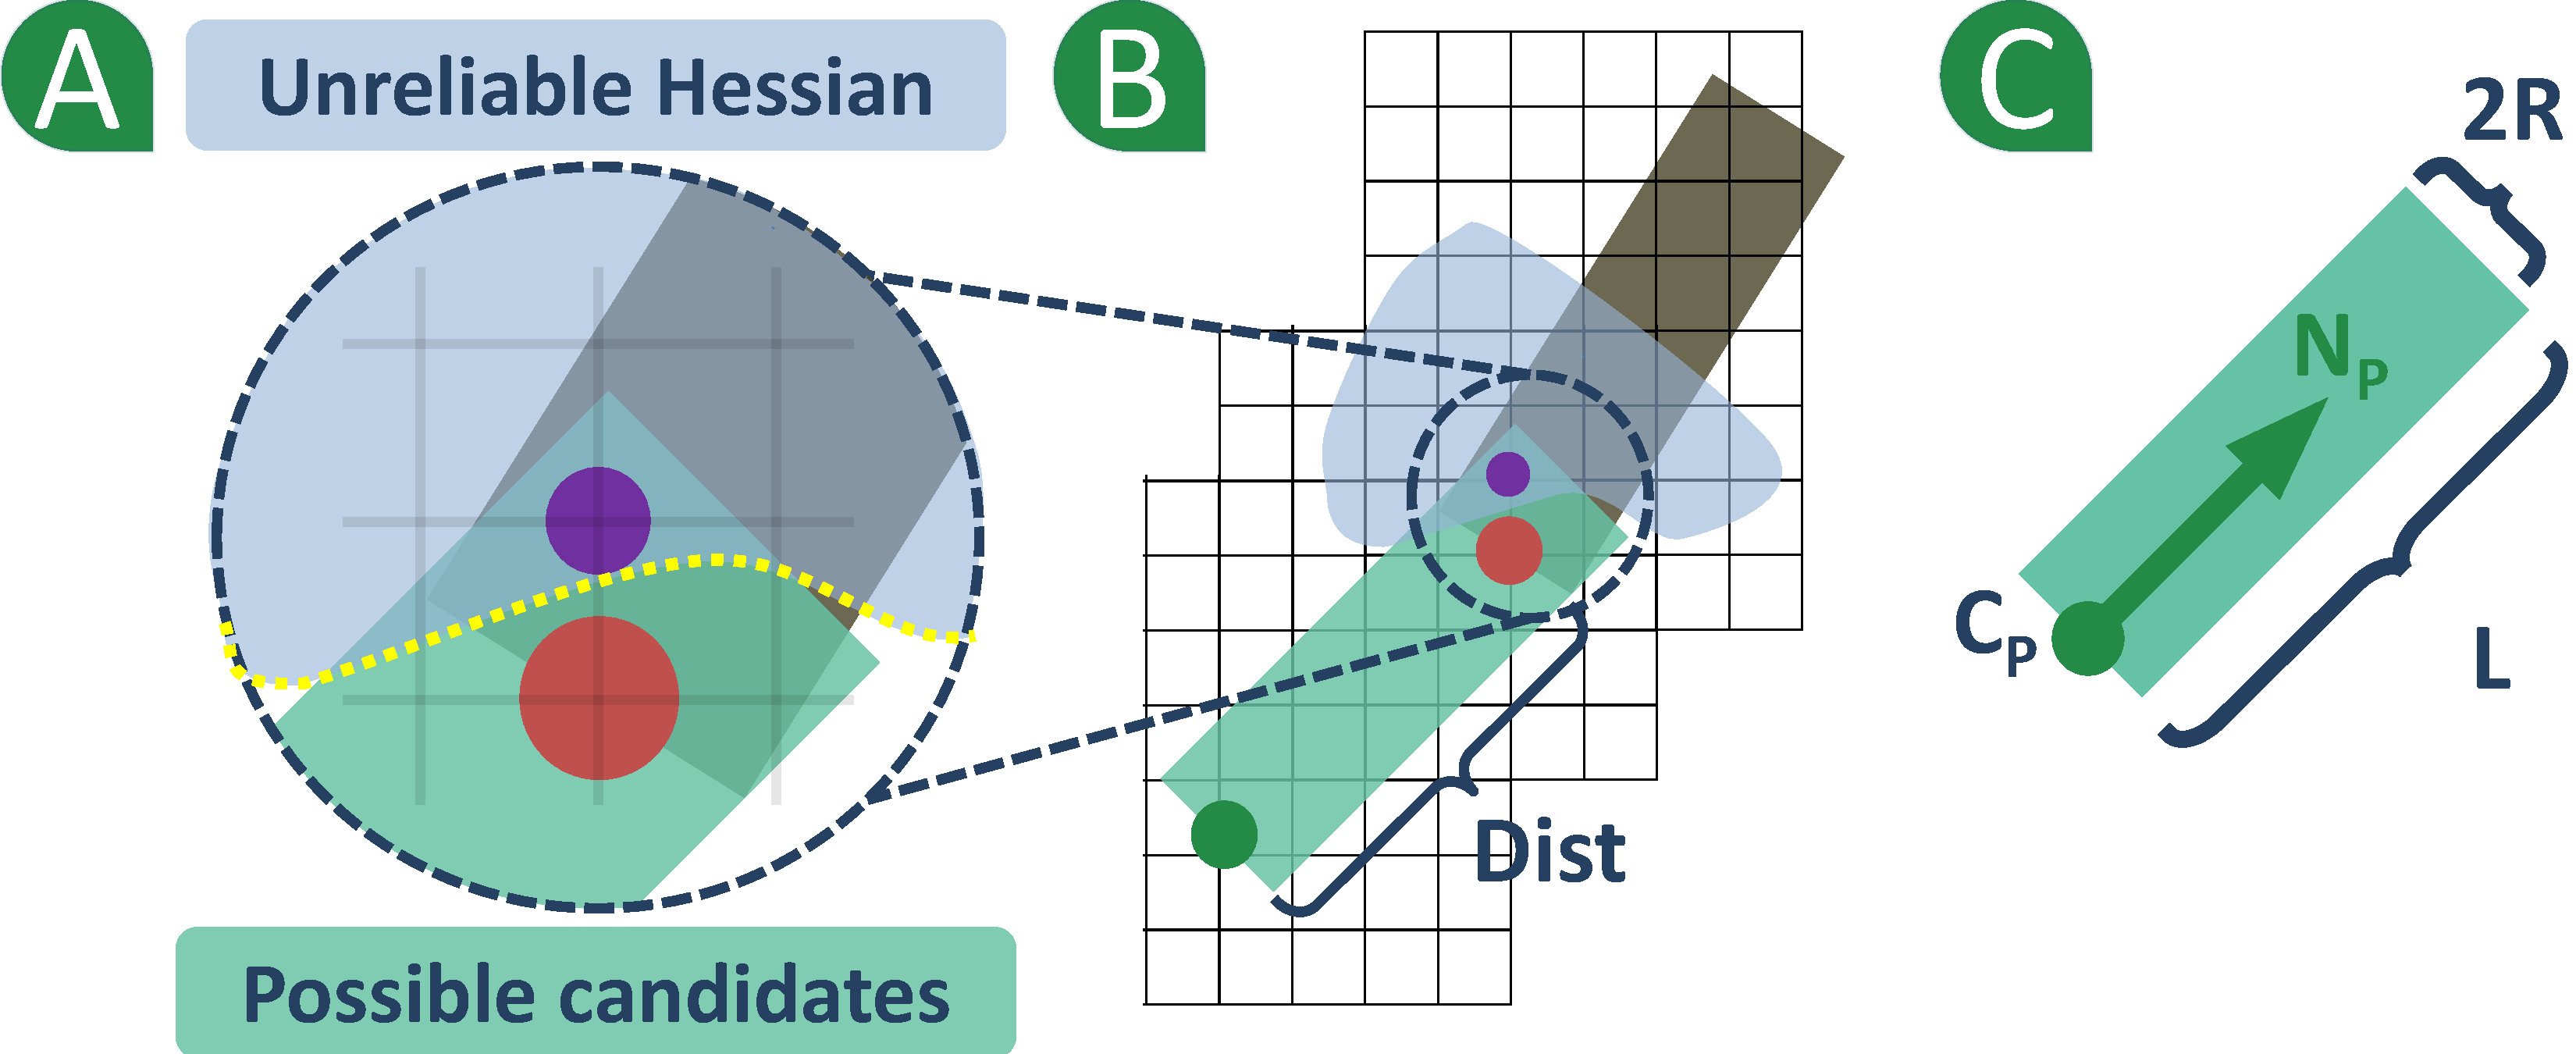
\includegraphics[ width=\linewidth]{images_pvis/mt_gen.pdf}
  \end{center}
  \vspace{-1em}
 \caption{MetaTracts generation: (b) Generation process. (a) Zoom in of the white marked region in (b). (c) Individual cylinder.}
  \label{fig:algo}
    \vspace{-1.5em}
\end{figure}
The set of vertices which are in the green region but not overlapped by blue are possible \textit{``candidate vertices"} for the start point of the next cylinder in a particular MetaTract. From these we select another grid vertex which will be the start point for the next cylinder.
%\begin{figure}
%\centering
% \includegraphics[width=0.25\textwidth]{imagesMetaTracts/angle-diff.png}
%\caption{Angle between the local orientation of two cylinders that are part of the same MetaTract.}
%\label{fig:angle-diff}
%\end{figure}
Based on assumptions on our data (local orientation and connectivity), the order of the candidate vertices is based on the following \textit{characteristics}:

\begin{itemize}[noitemsep]
\item \textit{Orientation similarity}: The orientation of the start points ($N_p$) for the consecutive cylinders should be similar. 
\item \textit{Large distance}: The MetaTracts should traverse the data using as few cylinders as possible. Thus, the distance between $C_p$ and the start point for the next cylinder should be as large as possible. We measure the distance of a candidate vertex from $C_p$ by projecting the Euclidean distance between them onto $N_p$. For example, in Figure~\ref{fig:algo}b the distance is measured as the Euclidean distance between the green and the orange vertices projected on to $N_p$. We refer to this perpendicular projection distance as \textit{`projected\_dist'}. 

\end{itemize}
% \begin{equation}\label{eqn:algo_1}
% d=\frac{1}{3}e^{(\frac{-angle^{2}}{\alpha^{2}})}+\frac{2}{3}(1-e^{\frac{-{PerpDist}^{2}}{\beta^{2}}})
% \end{equation}
We define a priority for each of the candidate vertices based on the above factors.
For each cylinder in a MetaTract, we put its \textit{candidate vertices} in a priority queue based on Equation \ref{eqn:algo_1}.
\begin{equation}
Priority = \gamma_1 e^{(-angle^2 / \alpha^2)} + \gamma_2e^{(-projected\_dist^2 / \beta^2)}
\label{eqn:algo_1}
\end{equation}
$\gamma_1$, $\gamma_2$ are the  weights ($\mathbb{R}_{\ge 0}$)  which decide how the priority depends on the affine combination of the two factors. For all our cases, we use $\gamma_1$ = $1 / 3 $ and $\gamma_2$ = $2 / 3$. In general, we suggest $\gamma_1 +\gamma_2 = 1 $ and $\gamma_1 \leq \gamma_2$. At each iteration, we pick the top element in the priority queue to generate the corresponding cylinder, and repeat the steps. Essentially, Equation~\ref{eqn:algo_1} selects a grid point which is furthest from the current point and is going in a similar direction. This approach tackles noise/errors in local orientation better than integral curves by looking at multiple choices for vertices and avoiding intra cell interpolation in an already noisy environment. 
In the example in Figure~\ref{fig:algo}b we select the orange grid vertex next and repeat the process. We do not select the purple vertex (Figure~\ref{fig:algo}c) because it is not a candidate vertex. If we generate tracts that have erroneous local orientations they will not be able to find further possible candidate vertices and are therefore removed. The MetaTracts generated are shown in Figure~\ref{fig:length_distribution}a. The MetaTracts are colored with the mean orientation direction mapped to the RGB space. Figure~\ref{fig:length_distribution}a also shows a single slice of YZ plane. Consistent orientation is a key intrinsic feature in the data which becomes visually pronounced.
We apply uniform, dense seeding to the XCT volume data to trace and generate the tracts of fiber bundles. Figure~\ref{fig:length_distribution}b shows the MetaTracts of a particular bundle colored according to their individual length.
%
MetaTracts in a given fiber bundle may extend the full length of the bundle and may feature different lengths as well as partial overlaps.
 
% \begin{figure}[h]
% \centering
% 	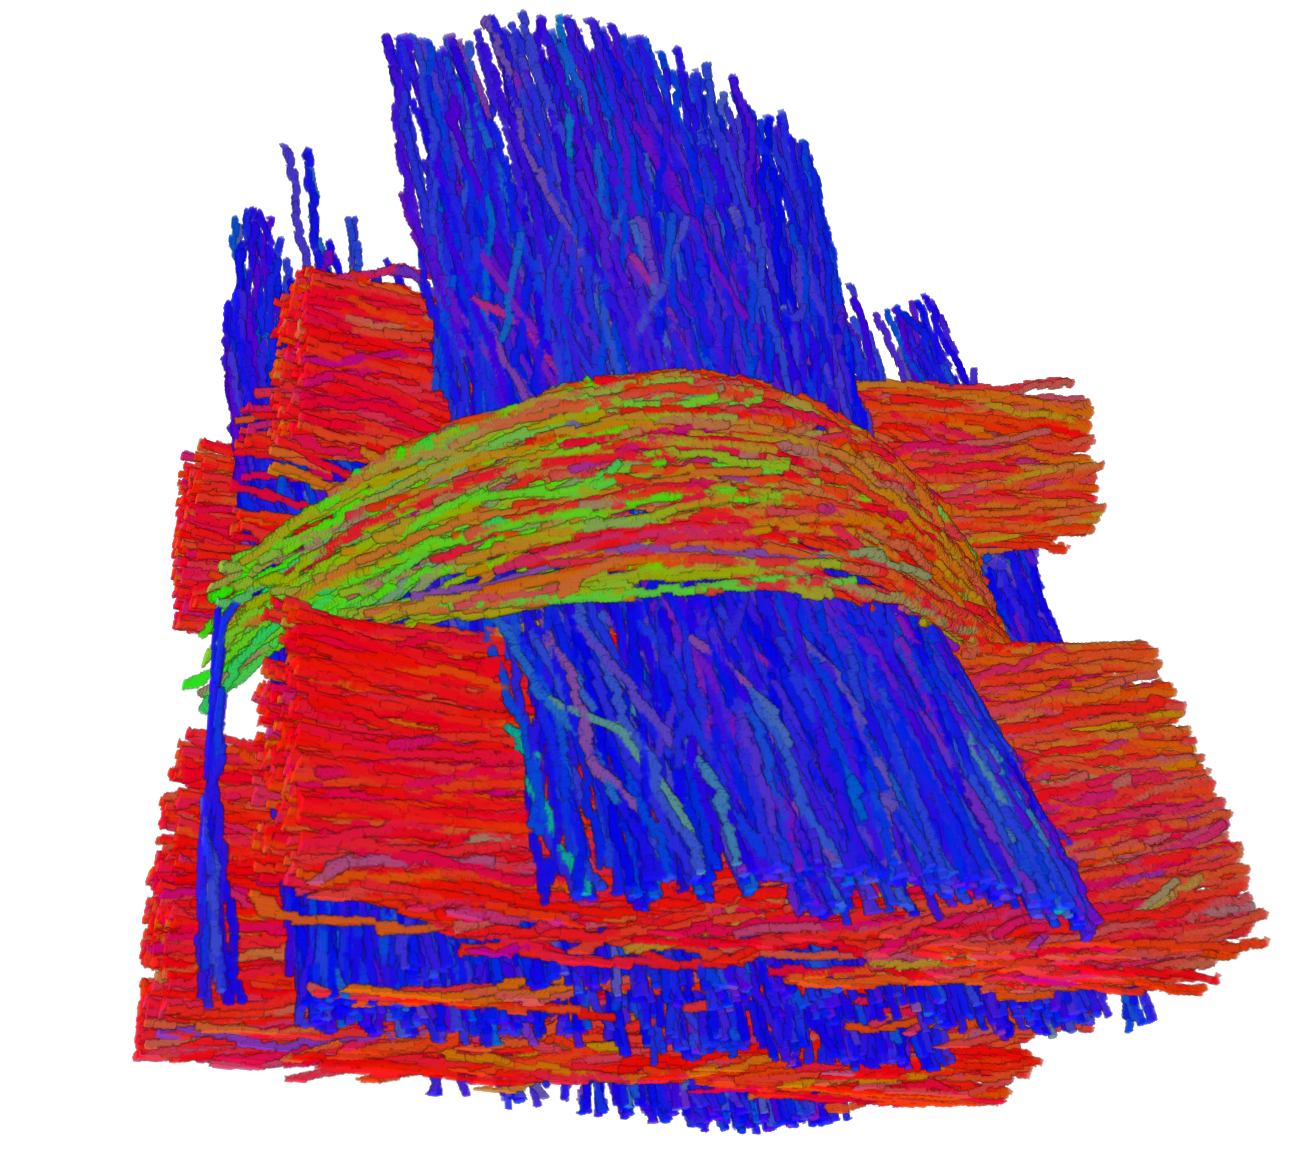
\includegraphics[ trim = 2cm 2cm 2cm 2cm, clip=true, width=0.3\textwidth]{imagesMT2014/MT_crop16_MT.png}
% 	\caption{MetaTracts, colored according to mean orientation mapped to RGB space}
% \label{fig:meta-tract}
% \end{figure}
 
%\begin{figure}
%  \centering
%  {\includegraphics[width=0.2\textwidth]{imagesMetaTracts/crop-13-tracks-1.eps}}
%  \caption{MetaTracts generated from one of our data sets. Each MetaTracts consists of cylinders. The mean local orientation, computed as the mean of the local orientations at the start point of each cylinder composing a particular MetaTract is mapped to the RGB space }\label{fig:meta-tracts}
%\end{figure}
%
 
%\begin{figure*}[htp]
%  \centering
%  \subfloat[]{\includegraphics[width=0.25\linewidth]{imagesMetaTracts/rplot-crop13.eps}}
% % \subfloat[]{\includegraphics[width=0.28\linewidth]{imagesMetaTracts/crop-13-tracks-clus-b.eps}}
%    \subfloat[]{\includegraphics[width=0.22\linewidth]{imagesMetaTracts/crop-13-tracks-clus-b-anno.png}}
%  \subfloat[]{\includegraphics[width=0.25\linewidth]{imagesMetaTracts/crop-13-tracks-clus-a.eps}}
%  \caption{Results from orientation based and hierarchical clustering. (a) shows the result of the K-means clustering with the data points projected to the top three Eigenvectors as the major axes, (b) shows the MetaTracts colored according to clustering results in (a), the corresponding clusters divide the MetaTracts according to their major orientation. (c) shows the result of hierarchical clustering of the results in (b), each orientation cluster (in this case 2) was divided into 7 classes.}\label{fig:clustering}
%\end{figure*}

%\begin{figure}
%  \centering
%  \subfloat[]{\includegraphics[width=0.22\textwidth,clip=true,trim=1cm 0cm 1cm 2cm]{imagesMetaTracts/rplot-crop13.eps}}
% % \subfloat[]{\includegraphics[width=0.28\linewidth]{imagesMetaTracts/crop-13-tracks-clus-b.eps}}
%    \subfloat[]{\includegraphics[width=0.3\linewidth,,clip=true,trim=1cm 0cm 2cm 0cm]{imagesMetaTracts/crop-13-tracks-clus-b-anno.png}}
%  \subfloat[]{\includegraphics[width=0.4\linewidth]{imagesMetaTracts/crop-13-tracks-clus-a.eps}}
%  \caption{Results from orientation based and hierarchical clustering. (a) The result of the K-means clustering with the data points projected to the top three eigenvectors as the major axes. (b) MetaTracts colored according to clustering results in (a). Corresponding clusters dividing the MetaTracts according to their two major orientations. (c) The result of hierarchical clustering of the results in (b), The two orientation clusters are divided into seven classes.}\label{fig:clustering}
%\end{figure}

%\subsection {Seeding}

%We apply uniform, dense seeding to the XCT volume data to trace and generate the tracts of fiber bundles.
%For our result we add a constraint. Only those grid vertices which have reliable hessians (Section~\ref{subsec:rh}). This restriction limits MetaTracts to  start from regions which have some underlying geometric structure. Regions that do not have reliable Hessians have poor local orientation and will not generate long MetaTracts. We also allow the user to selectively seed particular regions more densely.

\begin{figure}[tb]
\centering
	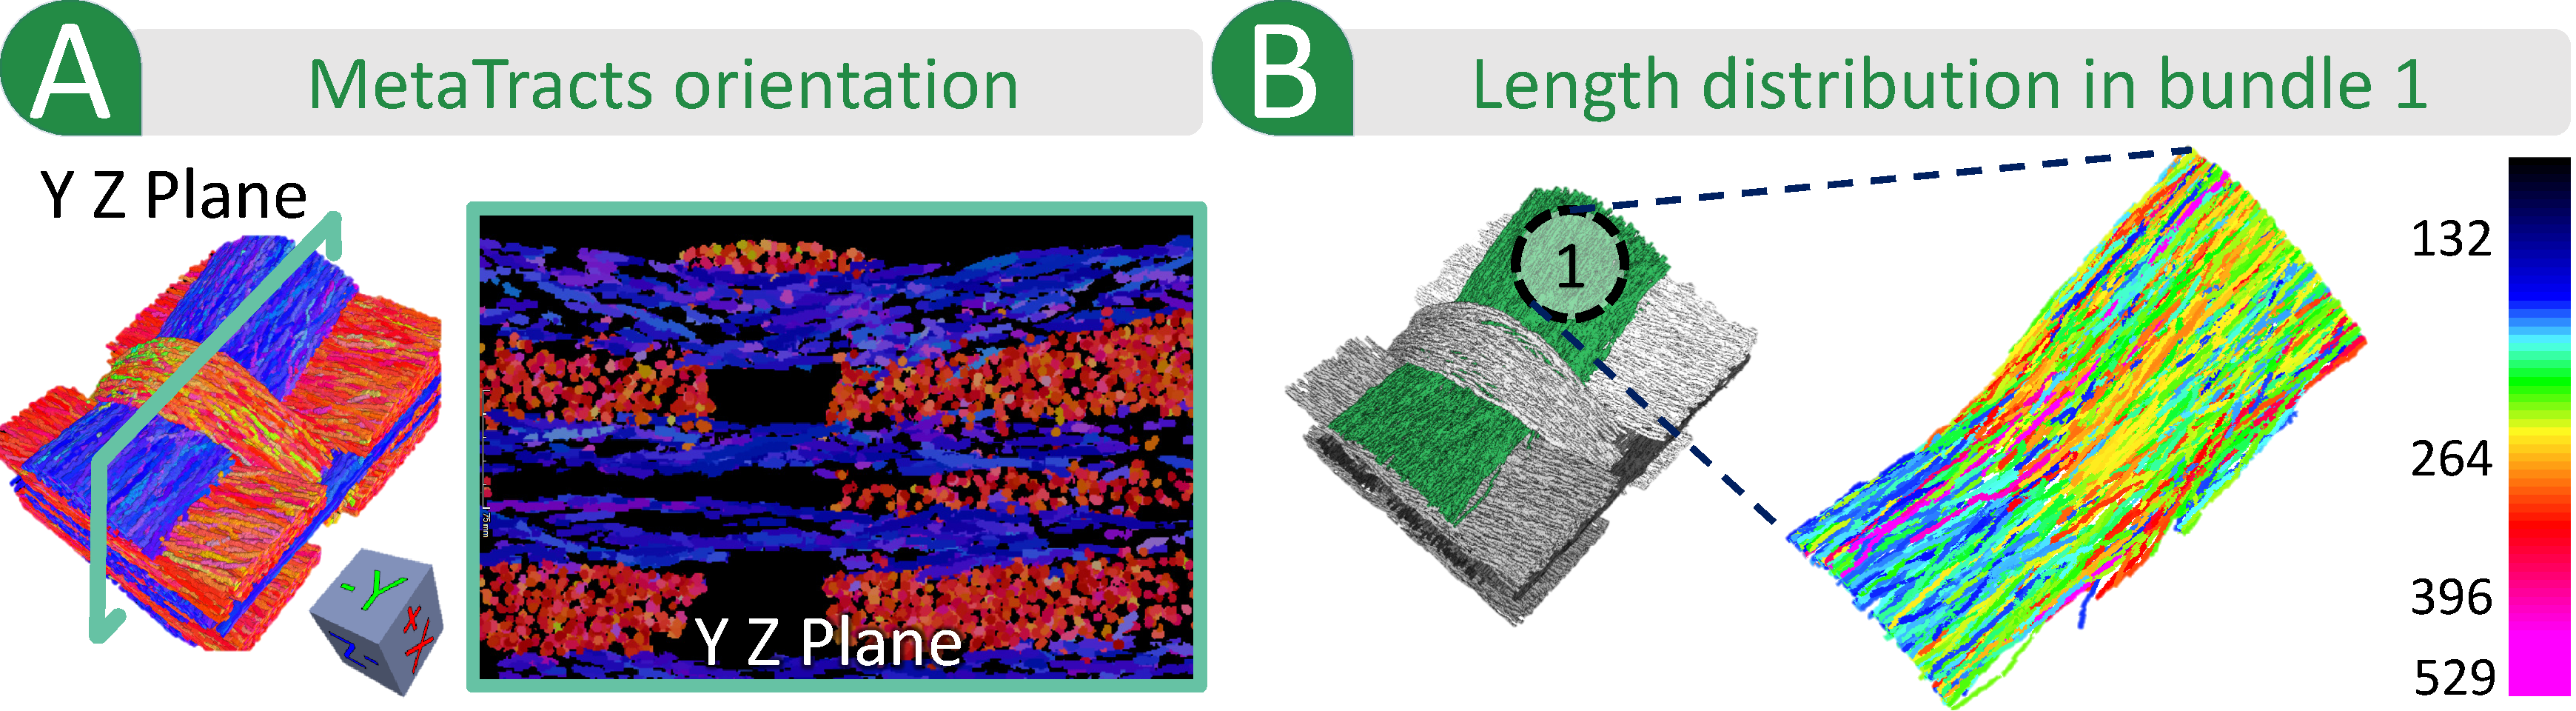
\includegraphics[width=\linewidth]{images_pvis/figure5.pdf}
	%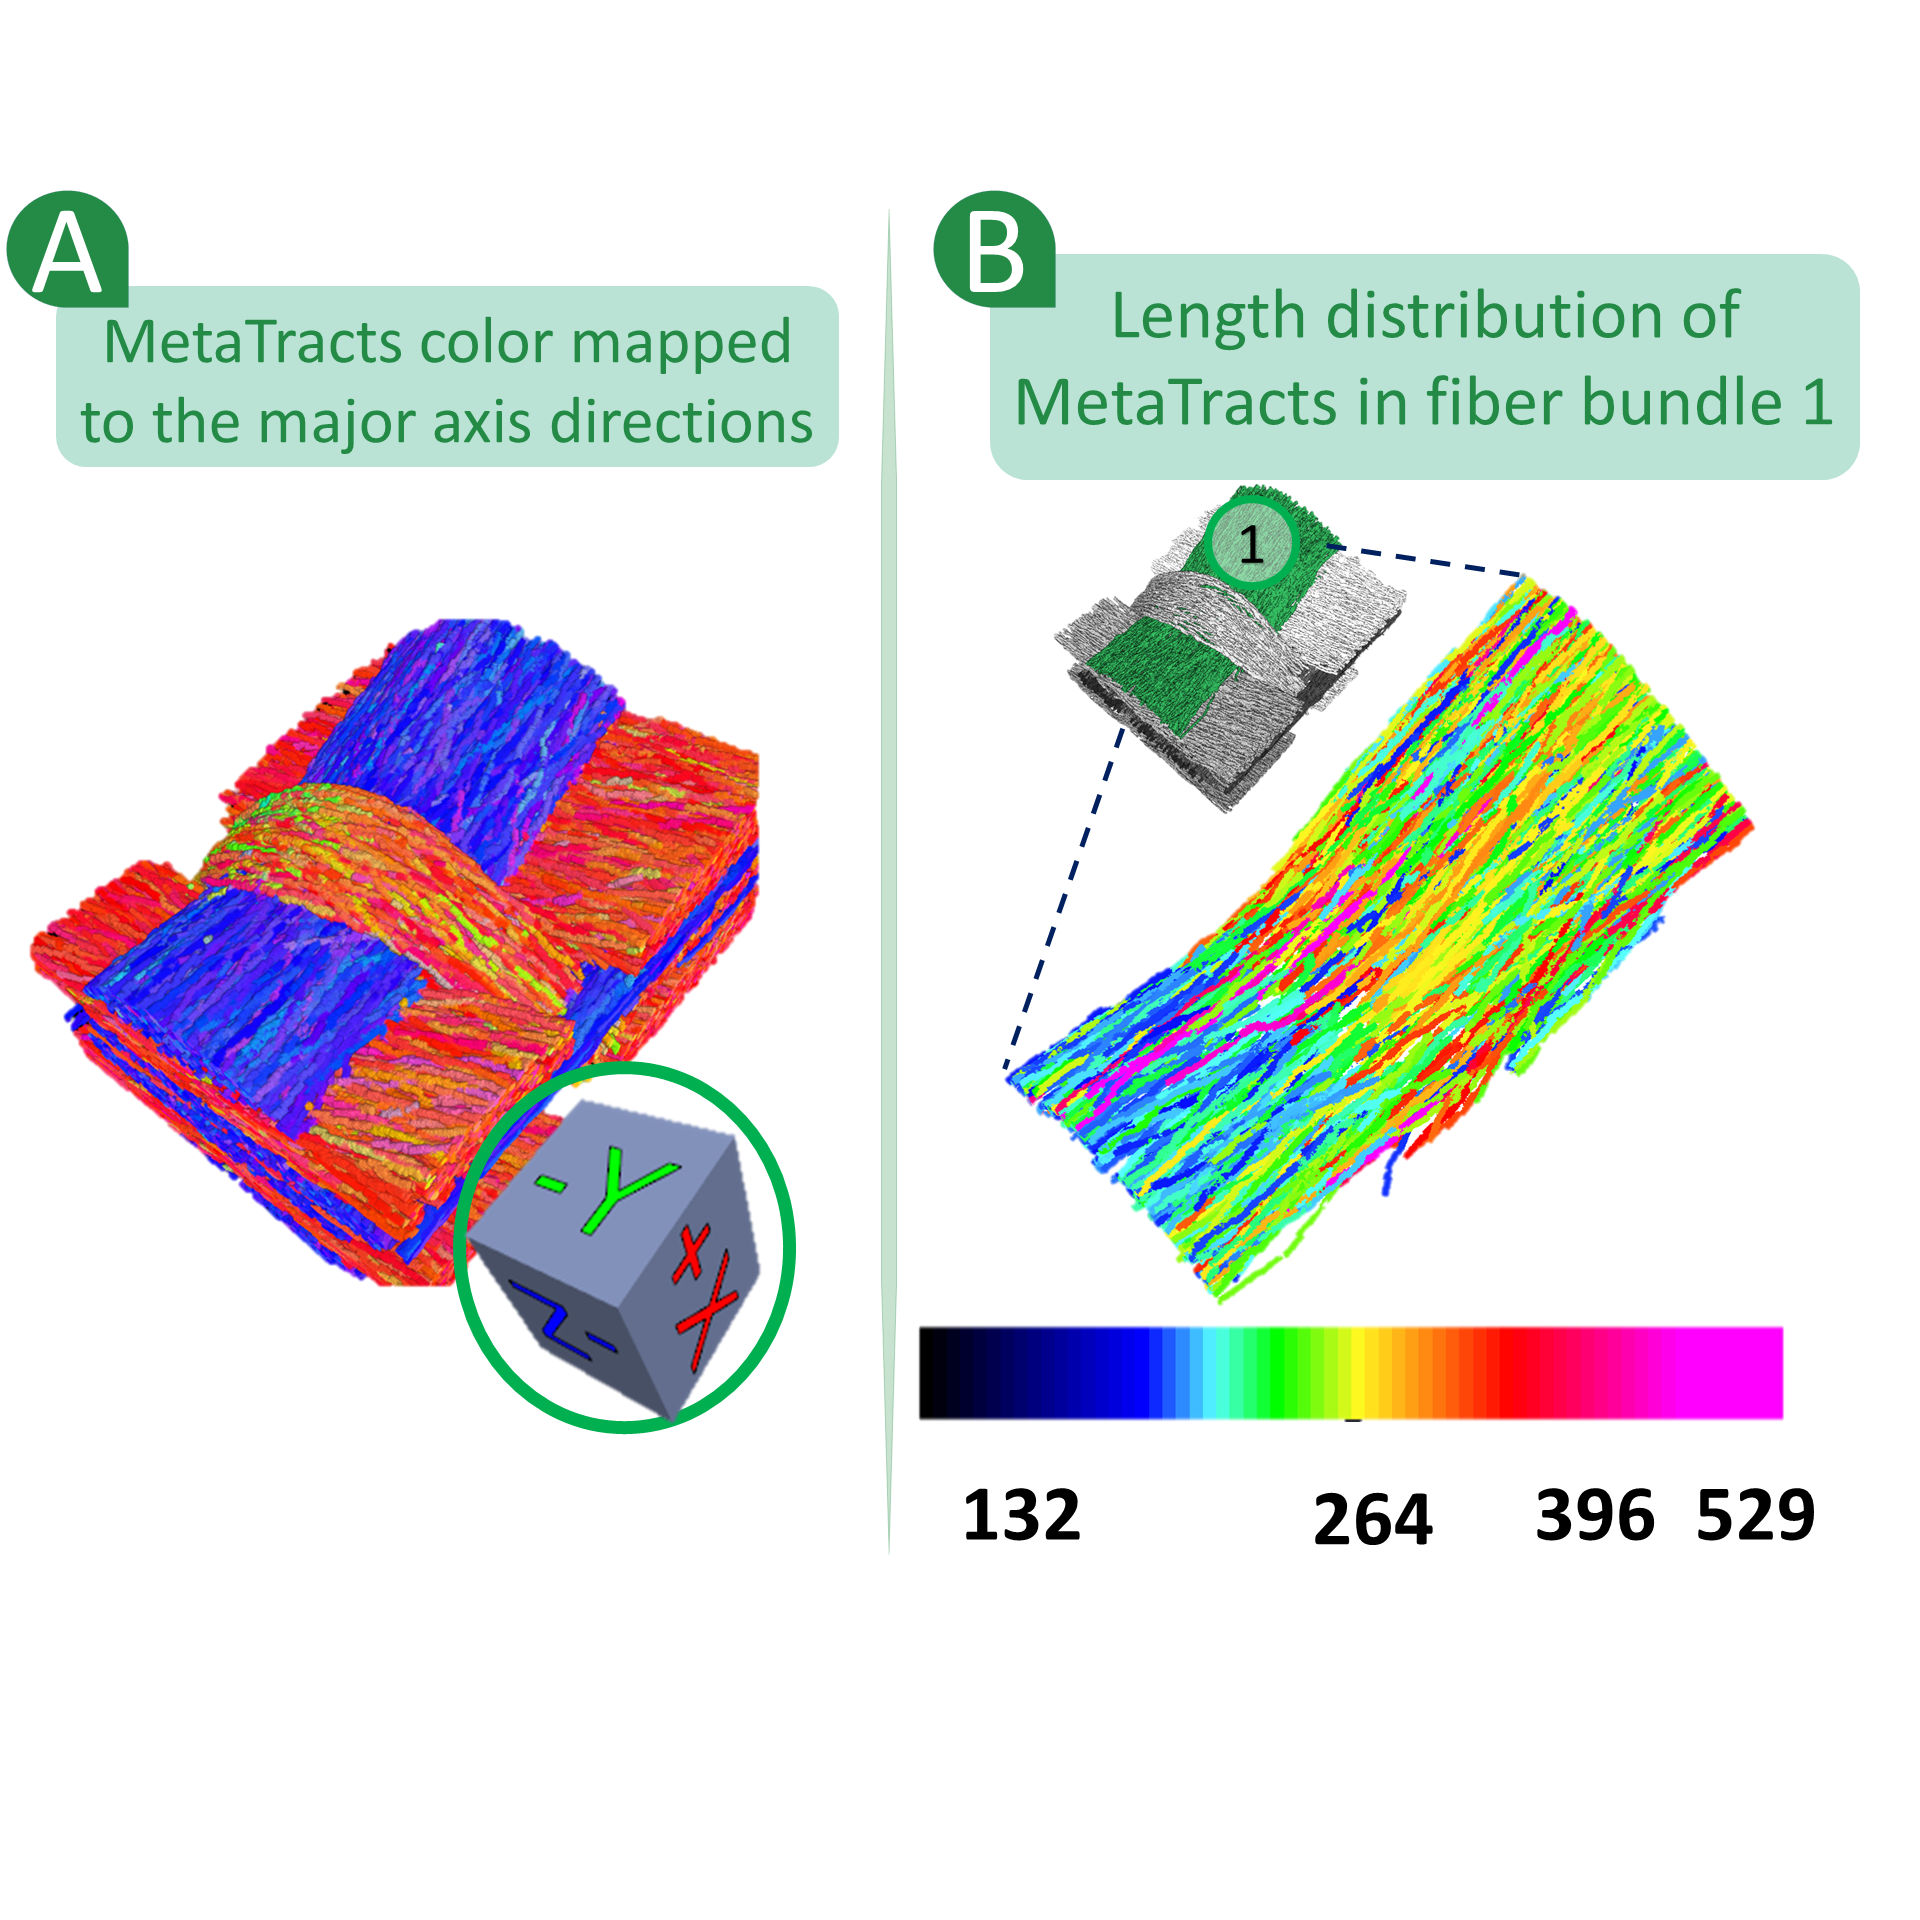
\includegraphics[width=0.45\textwidth,  trim = 0mm 100mm 0mm 50mm, clip]{imagesMT2014/image_length}
	\caption{(a) MetaTracts color-coded according to their mean orientations. (b) length distribution of individual MetaTracts for a particular bundle (unit for length is grid cube edge length:  $2\mu m$).}
	\label{fig:length_distribution}
\end{figure}


\section {Fiber Bundle Generation}
\label{subsec:fiber-bundles}

The set of MetaTracts generated by the previous step needs to be clustered in order to extract the final fiber bundles. 
Carbon fibers show both orientation and geometric proximity information, both of which can be used for clustering. Experimentally we found that the orientation measure was very reliable, while measures of geometric proximity had problems with partially overlapping fibers (Figure~\ref{fig:length_distribution}b). 
We also found that different clustering techniques performed preferably for different measures (Sec.~\ref{subsec:clus_choice}).  
So instead of creating a heuristic to artificially combine the orientation and geometric proximity measures, we first cluster based on orientation and then further subdivide each orientation cluster using geometric proximity. The two step clustering also made the problem more tractable and the parameters intuitive for the end users. For the orientation clustering, we use dimension reduction followed by K-means clustering. We then use hierarchical clustering to further subdivide each cluster based on the geometric proximity measures. 

%However, in approaches developed for DTI fibers such as proximity based distance measures and clustering, the short comings of the fiber tracking techniques are generally not discussed and it is assumed that fibers in each bundle are of similar lengths and which traverse the data end to end. This is not the case for noisy data such as ours.
%In Figure~\ref{fig:hclust_issue_a} proximity based distance, for example mean of the minimum distances between points on MetaTracts might falsely find the red MetaTract being closer to the blue, than the orange MetaTract. 
%We also note from Figure~\ref{fig:meta-tract} and from domain knowledge that all our fibers are well separated by orientation. Thus instead of directly applying hierarchical clustering to our data,
%we first cluster based on orientation using a simple measure.
%We use domain knowledge to divide the clustering into two intuitive parts:because of the woven nature of fiber bundles in our application domain we first cluster in terms of orientation. This has the advantage of being able to separate tracts which might be close in an Euclidean space but traveling in different direction. We introduce a simple orientation based similarity measure (sec~\ref{subsec:ori-sim-mes}). Finally, for each of these clusters we re-cluster in terms of distances measured in a Euclidean space (sec~\ref{subsec:dist_clustering}).


\subsection {Orientation based clustering}
%We use the inherent features expressed as weaving pattern of our data to pre-cluster the metaTracts into the number of classes based on the major directions of the pattern.
%It is important to note that this step broadly divides the MetaTracts into classes based on the major orientations and not individual fiber bundles. 
This step divides the individual MetaTracts into classes based on their major orientations. In order to cluster MetaTracts going in the same directions, we use a spectral embedding technique called Laplacian eigenmaps as originally introduced by Belkin and Niyogi \cite{Belkin01}. An eigenvalue problem is solved, which maps the manifold embedded in the graph into a lower dimensional space while preserving the graph structure.
Let $G$ be the graph, we compute the eigenvalues and eigenvectors for the generalized eigenvector problem $L\textit{\textbf{f}}=\lambda D\textit{\textbf{f}}$,
%\begin{equation}\label{equn:eigenMaps}
%L\textbf{f}=\lambda D\textbf{f}
%\end{equation}
where $D$ is the diagonal weight matrix and $L$ is the Laplacian matrix. The eigenvector \textbf{${f}_{0}$} corresponding to the eigenvalue 0 is left out and the next $m$, {\textbf{${f}_{1}$} through \textbf{${f}_{m}$}} eigenvectors are used to embed in an $m$-dimensional space (see Sec.~\ref{sec:param_choices} for values of m).
In our case, each MetaTract is a data point. We introduce a simple \textit{orientation based similarity measure}. There is no spatial information involved, just a partition of the MetaTracts based on orientation which is already inherent in the data.
Following this, given a pair of  MetaTracts, we define the edge weights between two tracts as the cosine of the maximum angle between the local orientations ($N_P$) of all pairs of start points ($C_P$) between the two MetaTracts. The edge weights give a distance matrix representing the distance between each pair of points. Using the Belkin and Niyogi algorithm we ``embed" these points in a low dimensional space where the Euclidean distance between points approximates the distance between points given by the distance matrix. 
%
%August 13 2014
%For all our tests the fibers were then embedded in a $\eta$ low dimensional space. The number of dimensions in the high dimensional space is equal to the number of datapoints or the number of MetaTracts in our case.
%For all our test cases we set $\eta$ to be five (see sec~\ref{sec:param_choices} for parameter choices for $\eta$.).
%  
We used conventional K-means for clustering this lower dimensional space. Here $K$ is supplied by domain knowledge of the number of major fiber bundle directions of the woven structure.
For our test case there are two major directions of the fiber bundles and $K$ was set to 2. Due to the advantages offered by the dimensionality reduction, even if there are curved fiber bundles the user has to provide just the major fiber bundle directions of the weaving pattern. Figrue.~\ref{fig:orientation_clustering}b shows the result of the K-means clustering with the data points projected to the top three eigenvectors as the major axes. As is expected there is a clear distinction based on fiber orientation. Figure~\ref{fig:orientation_clustering}a,c shows the MetaTracts colored according to clustering results.


\begin{figure}[tb] 
  \centering  	
  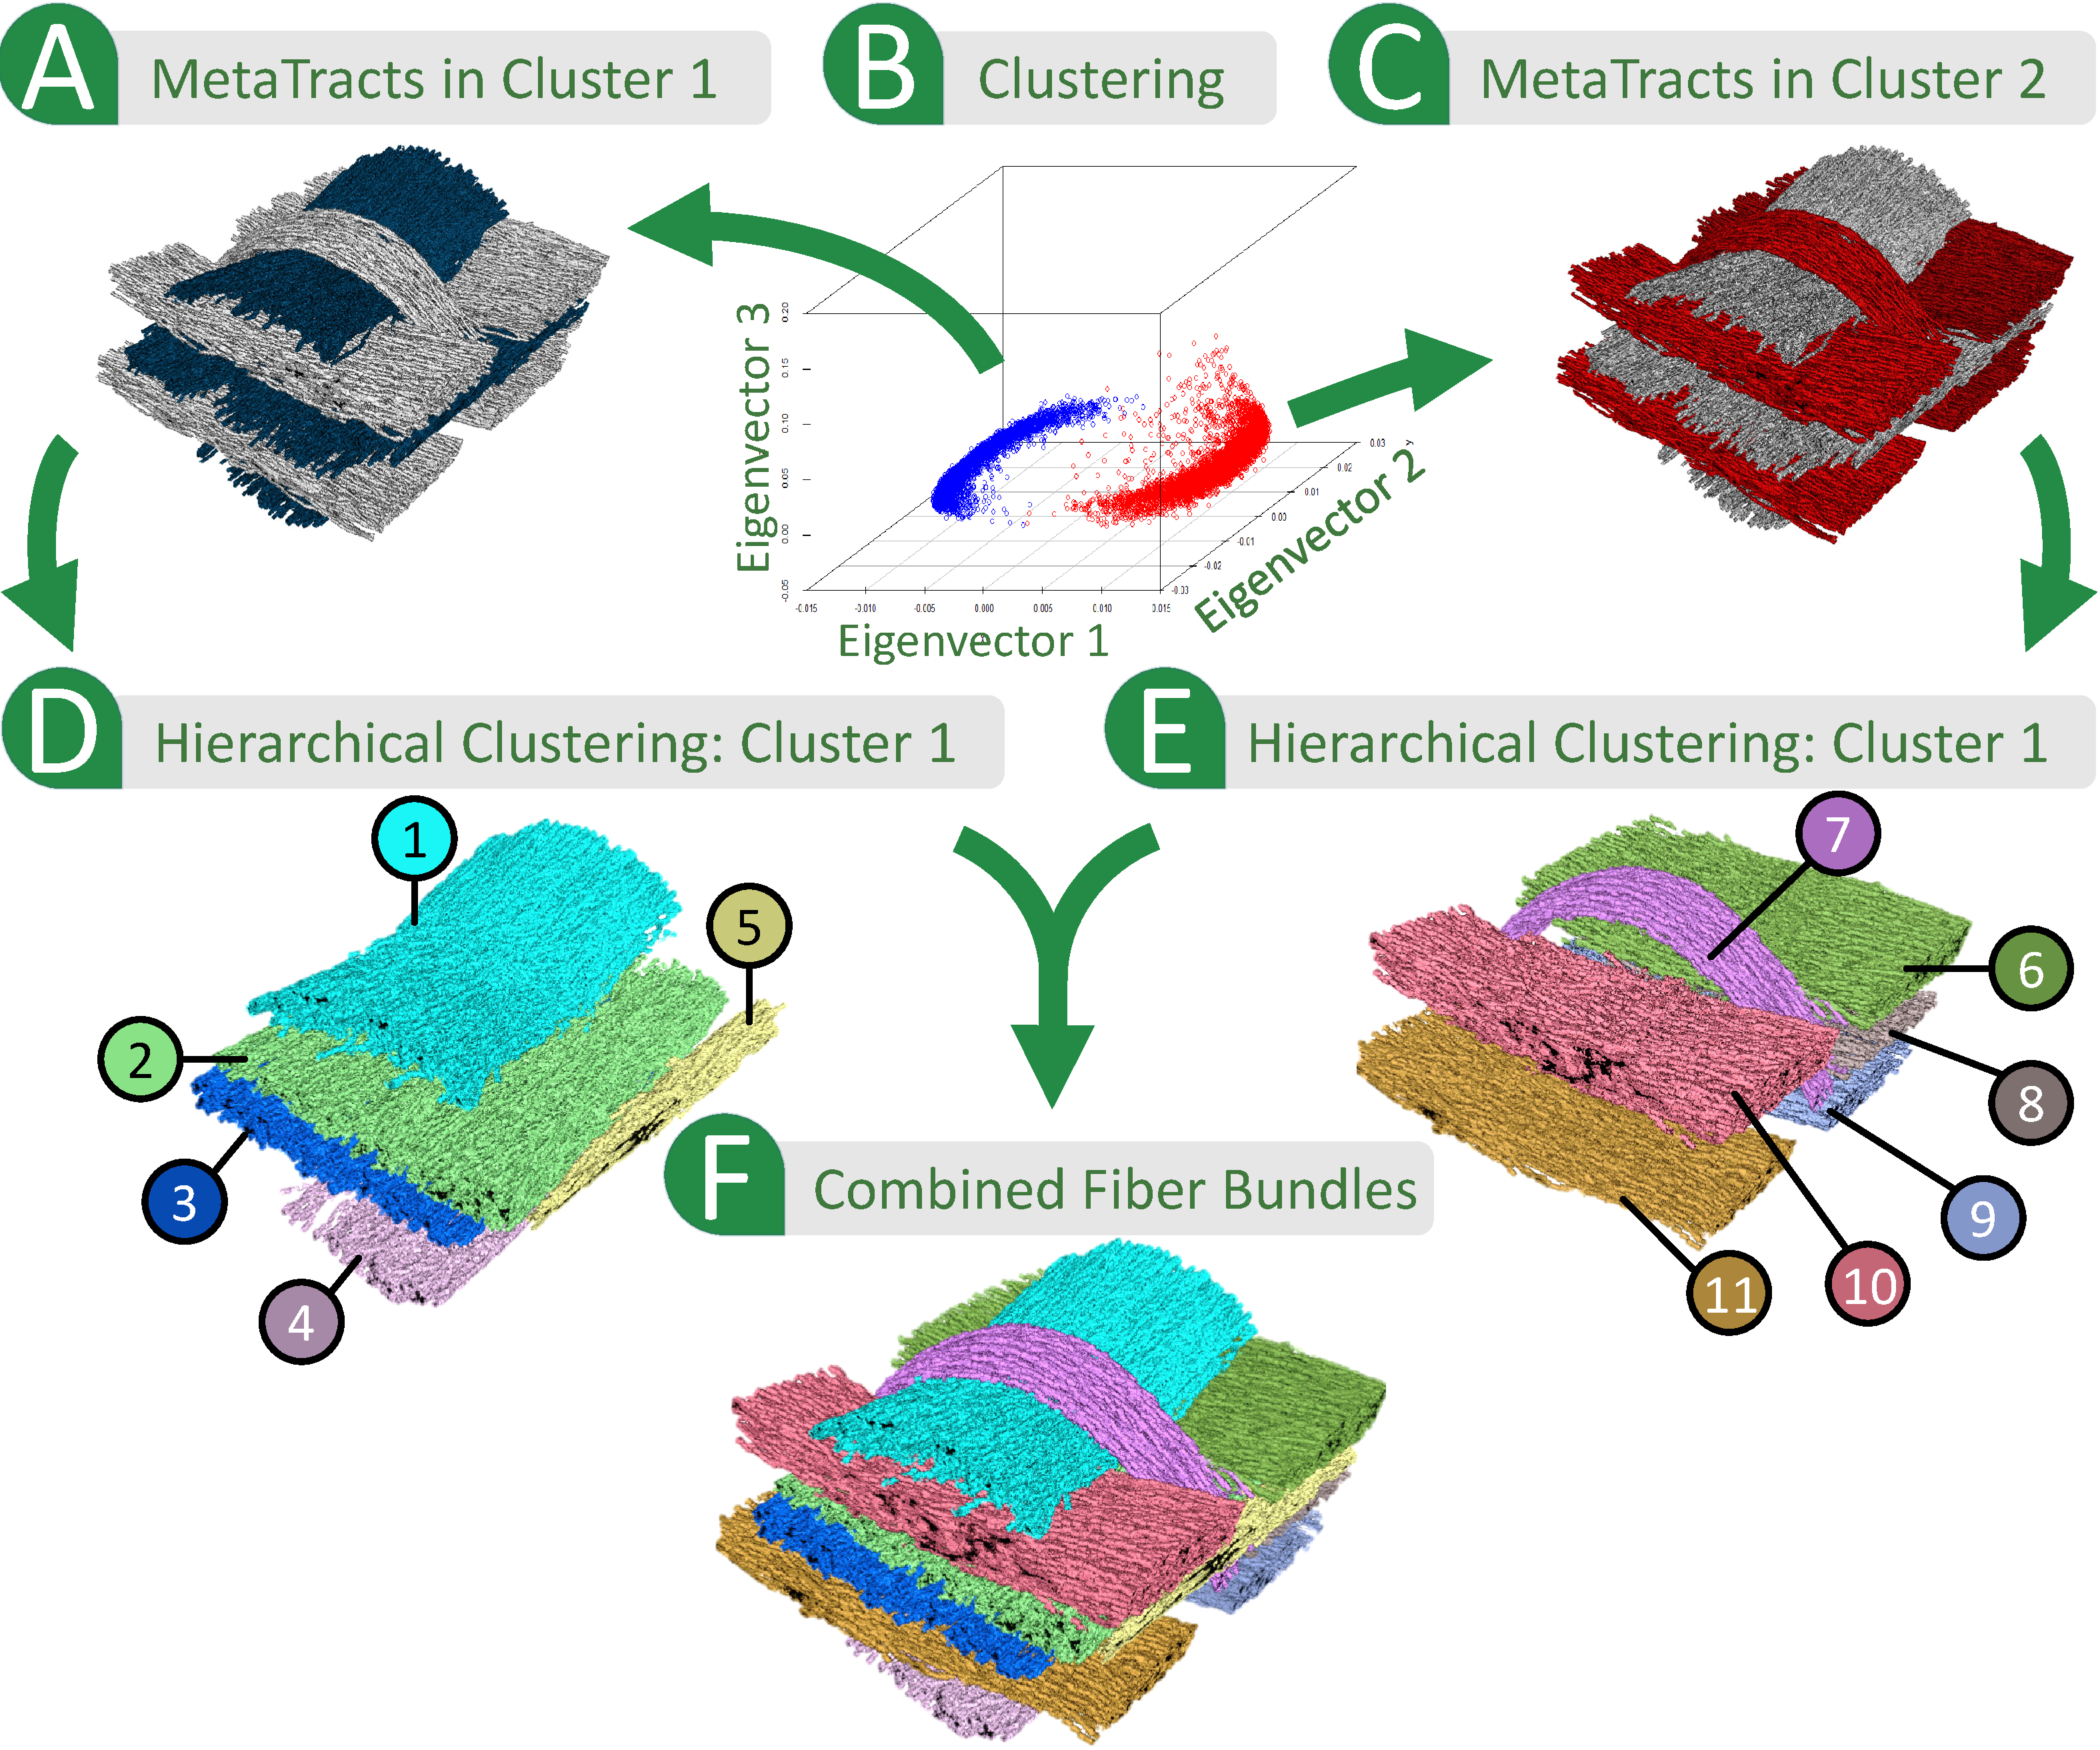
\includegraphics[width=\linewidth]{images_pvis/clustering.pdf}
   \vspace{-1.5em}
  %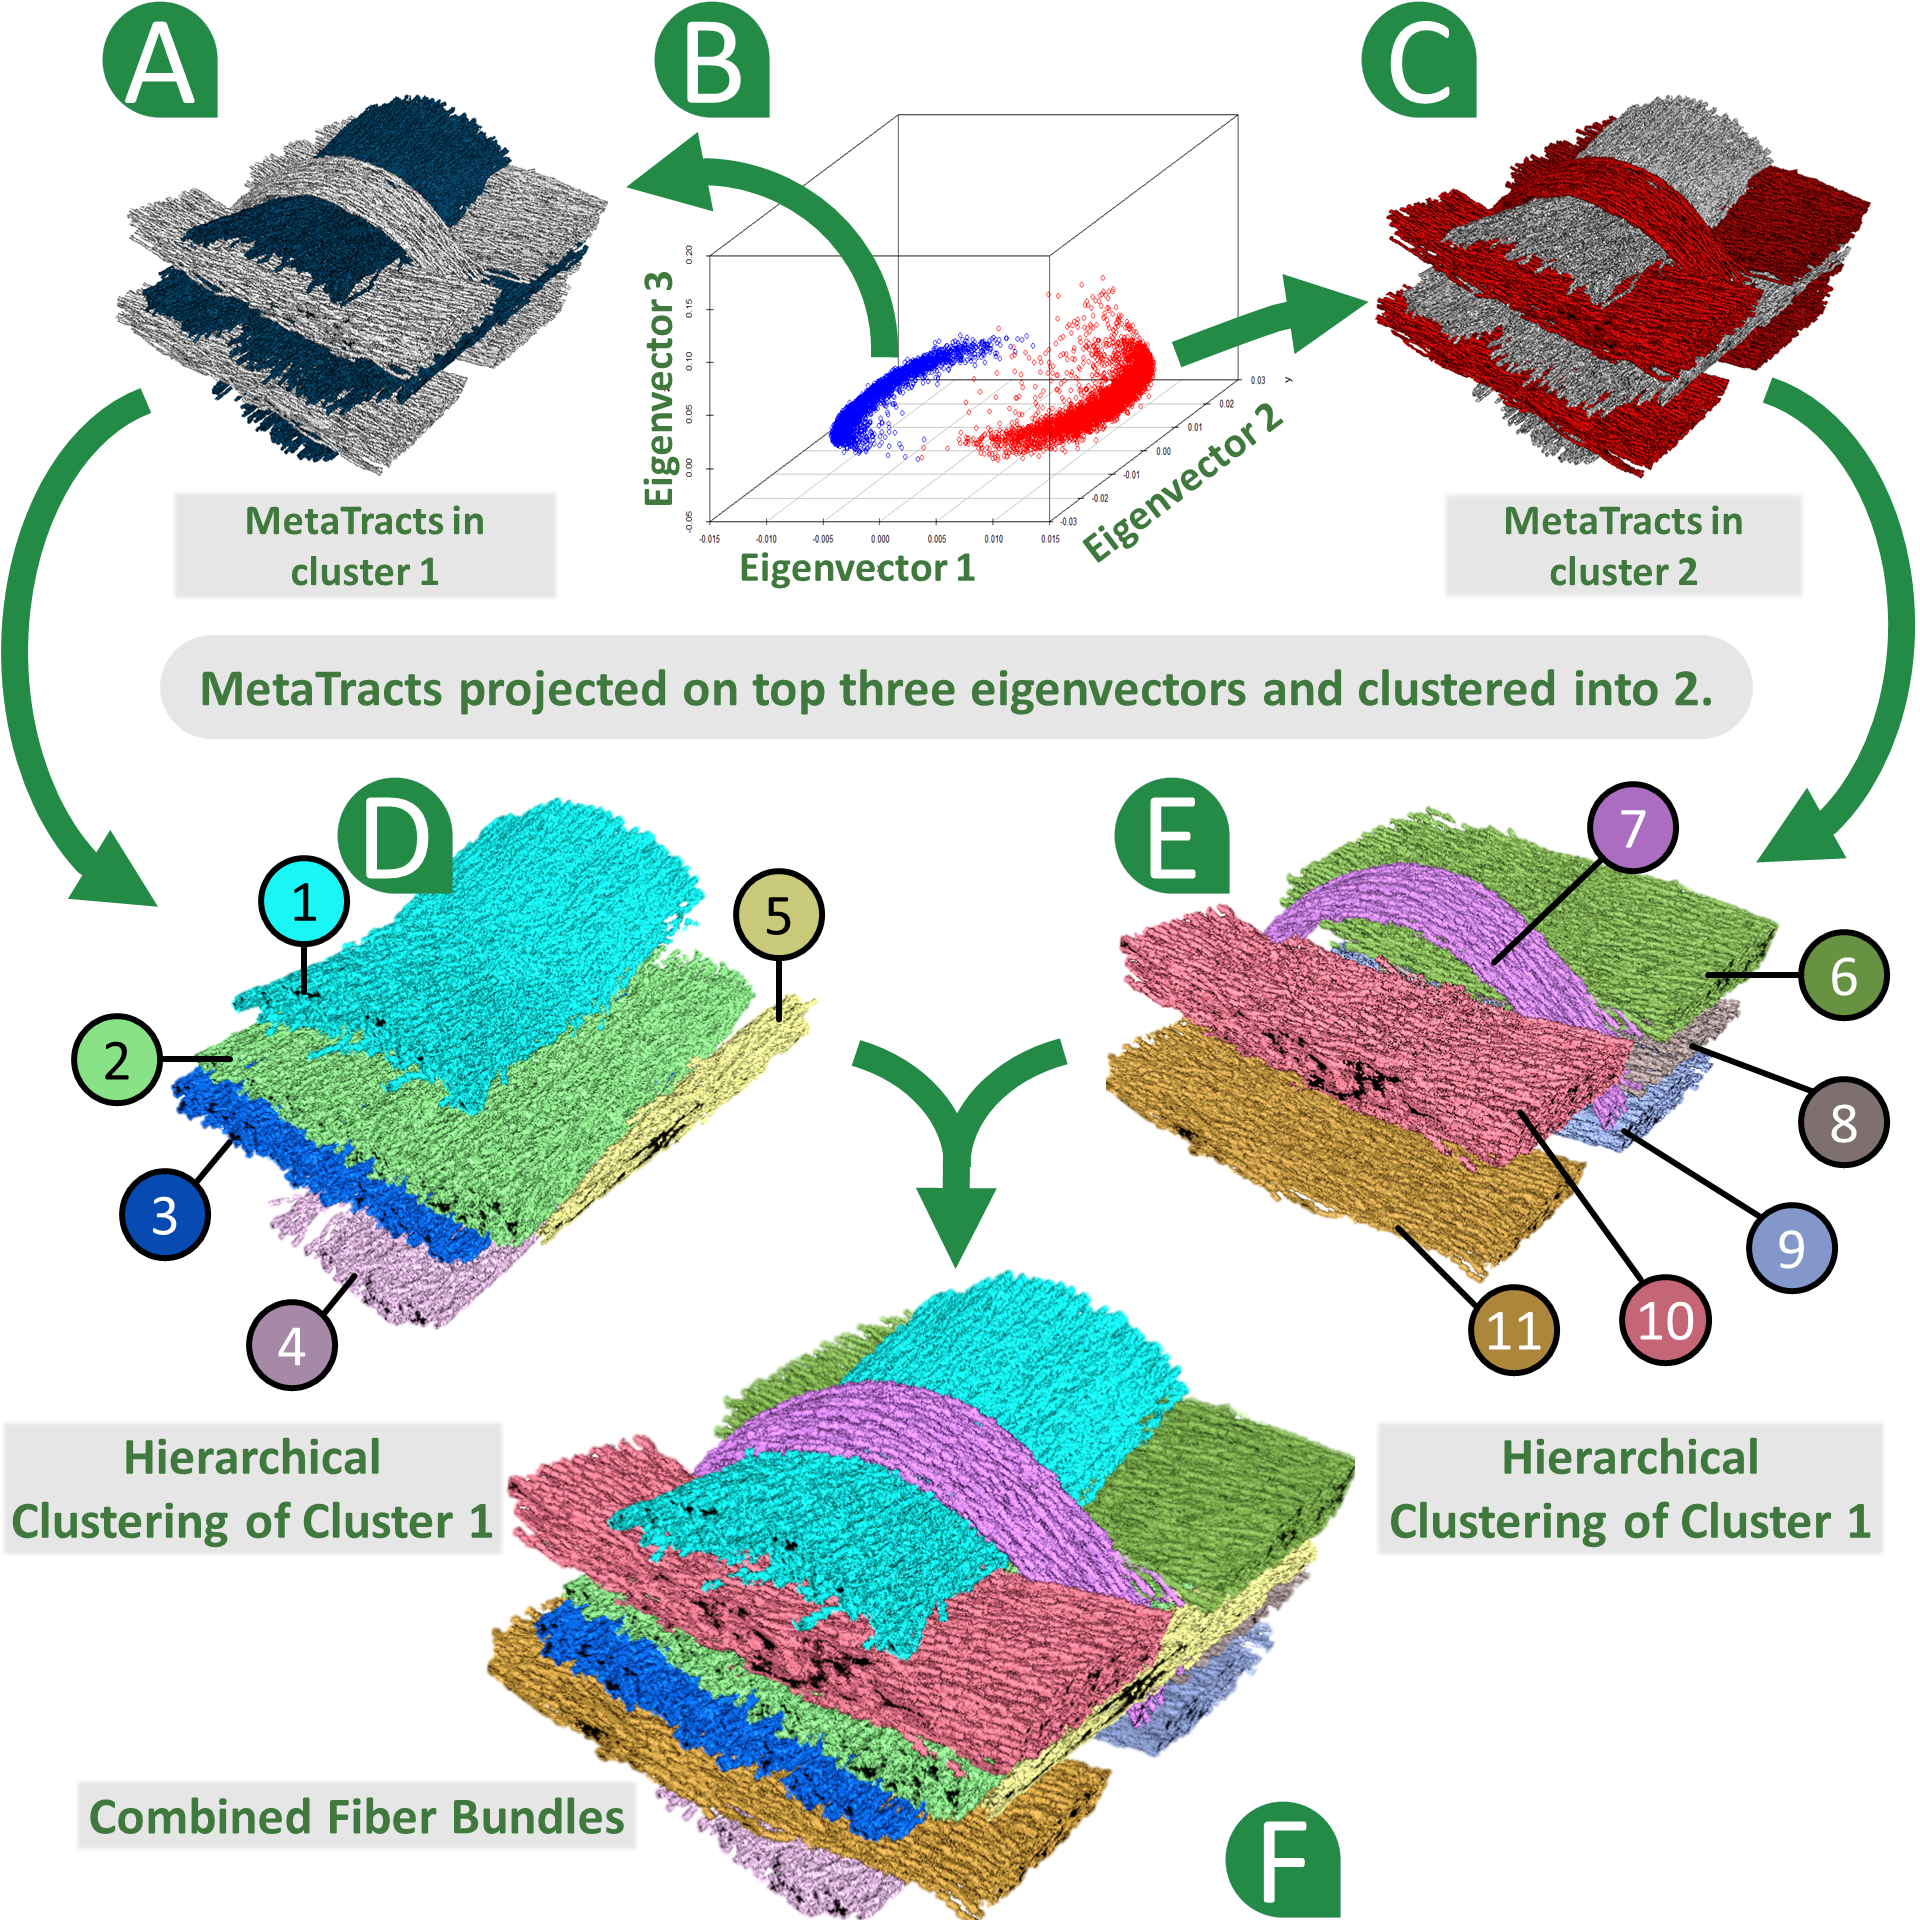
\includegraphics[width=0.45\textwidth]{imagesMT2014/image_clustering}
  	\caption{(b) Result of K means clustering with data points projected to the top three eigenvectors as major axes. (a) MetaTracts belonging to orientation cluster 1. (c) MetaTracts belonging to orientation cluster 2. MetaTracts in gray (a,c) show context.
  	(d,e) shows the result of distance based clustering on the orientation cluster. (f) shows the combined result. }
  \label{fig:orientation_clustering}
  \end{figure}

%\subsection {Distance based clustering}
%\label{subsec:dist_clustering}
%We now apply "single-linkage" hierarchical clustering~\cite{Moberts2005} to the results of the orientation clustering results.
%If we assume each fiber is represented as a set of points($C_P$) then the distance between two MetaTracts is computed as the minimum of the directed Hausdorff (maximum of the minimum euclidean) distances between points on the MetaTracts. Hierarchical clustering has one parameter, which is the number of clusters (h). Single linkage clustering inspite of it's advantages and  wide spread use, though suffers acutely in the presence of outliers.
%
%\begin{figure}[h]
%  \centering
%  	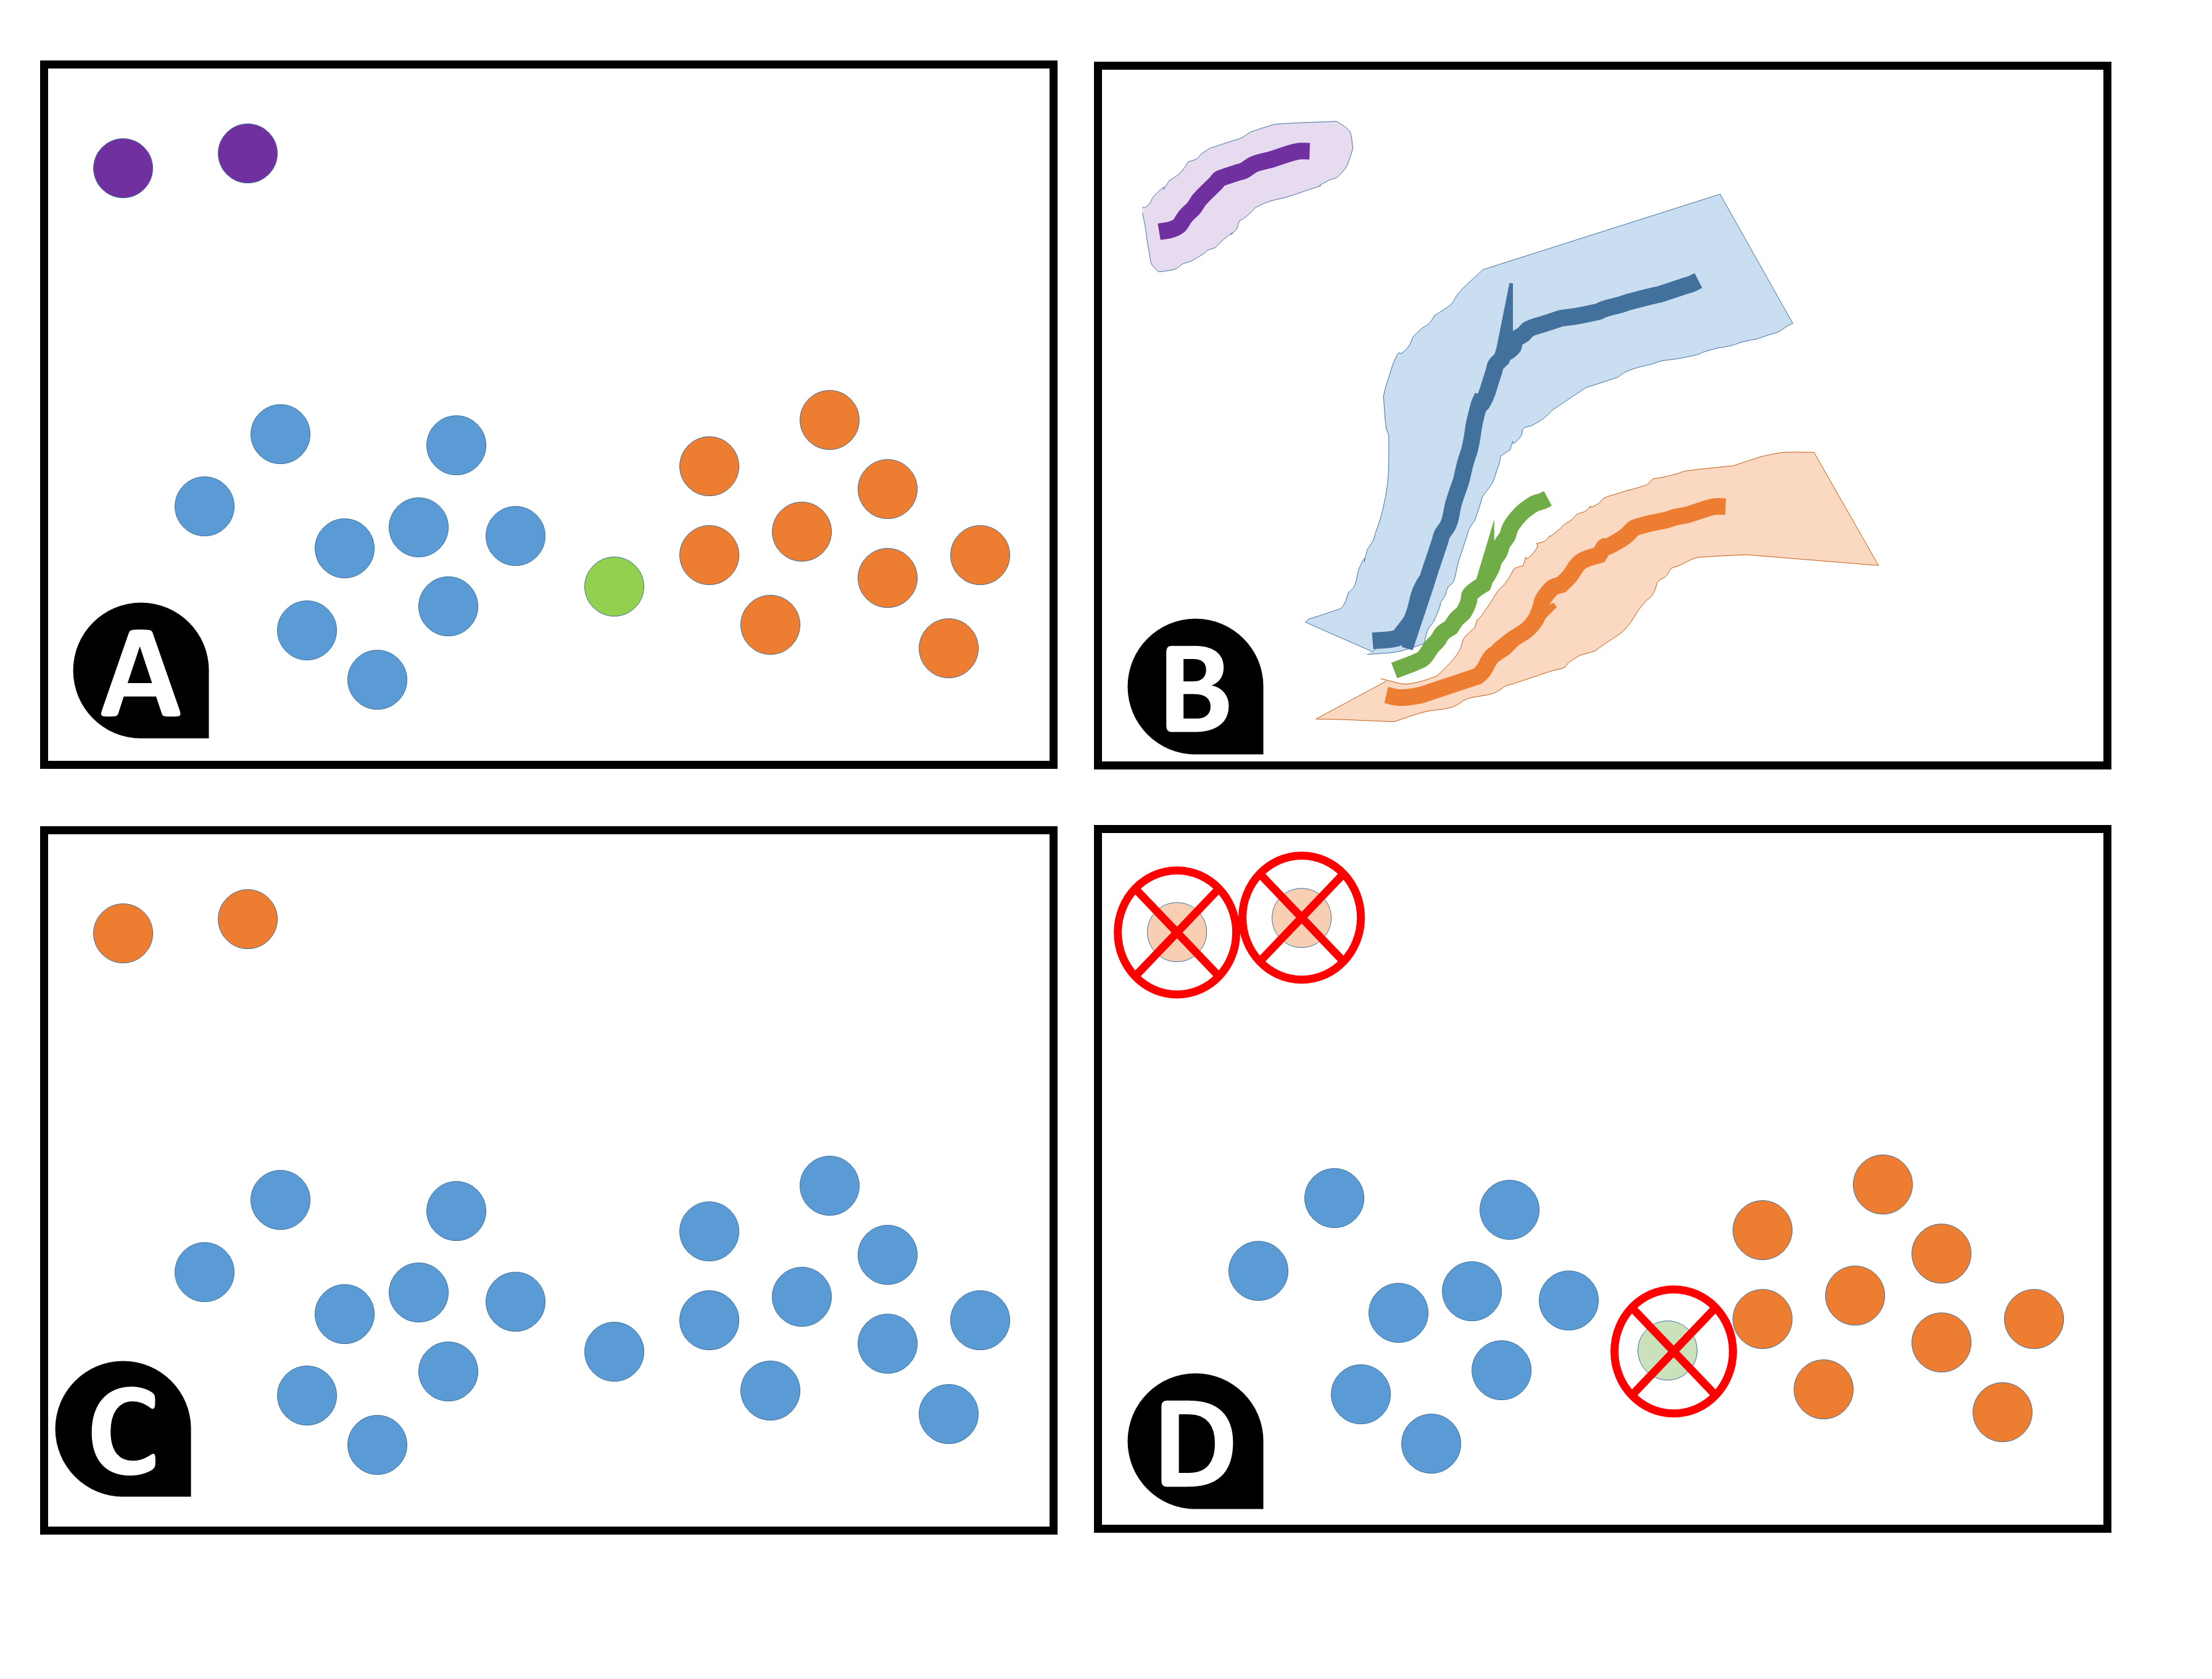
\includegraphics[ trim = 2cm 2cm 2cm 2cm, clip=true, width=0.3\textwidth]{imagesMT2014/clustering_probs_B.png}
%  	\caption{test}
%  \label{fig:cluster_prob_B}
%  \end{figure}
%For example Figure~\ref{fig:cluster_prob_B}B shows two main bundles (blue, orange), one outlier which has close proximity to both bundles (green) and another outlier far away from both the bundles (purple).
%Figure~\ref{fig:cluster_prob_B}A shows some sample MetaTracts from the bundles as points in a euclidean space.
%Setting h to 2 and performing single linkage hierarchical clustering would give a wrong result (Figure~\ref{fig:cluster_prob_B}C) It would create the outlier as a separate class instead of breaking the larger group. As a robust solution to the problem we perform hierarchical clustering iteratively. At each step removing clusters which have low cardinality(this is a common practice). However, we also remove elements from each cluster which have length lower than the median length of the fibers in the bundle. After a few iterations a stable state is reached where the outliers are removed and the clustering into bundles is robust(Figure~\ref{fig:cluster_prob_B}D).
%\begin{figure}[h]
%  \centering
%  	\includegraphics[ trim = 1cm 1cm 1cm 1cm, clip=true, width=0.3\textwidth]{imagesMT2014/final_clustering_A.png}
%  	\caption{Results of MetaTracts clustering. A: shows the X orientation cluster, clustered into 10 clusters. B: shows the Z orientation cluster, clustered into 10 clusters. Clusters with cardinality less than 10 are not shown. C: shows a close of the curved bundle extracted from the data. D: shows the original data for comparison.}
%  \label{fig:cluster_final_A}
%  \end{figure}
%  Figure~\ref{fig:cluster_final_A}(A,B) show the results of clustering each orientation bundle into ten clusters. Clusters with cardinality less than ten are not shown. Figure~\ref{fig:cluster_final_A}C shows the closeup of the curved bundle and Figure~\ref{fig:cluster_final_A}D shows the original data for reference. Single linkage clustering is very robust to the over-estimation of "h". A very large value of "h" would still keep the main clusters intact and create smaller  clusters with low cardinality which qualitatively does not degrade the results at all.

  
\subsection{Distance based clustering}
 \label{subsec:dist_clustering}
Orientation clustering uses only orientation information. To subdivide the oriented clusters into fiber bundles, we need to include further information about the geometric proximity between MetaTracts. We use the directed Hausdorff distance for distance based clustering.
Each MetaTract is represented as a set of points ($C_P$). Formally, the directed Hausdorff distance from point set $P$ to point set $Q$ is defined as 
$H_{dir}(P,Q) = max_{p \in P} min_{q \in Q} d(p,q)$ .
The Hausdorff distance is defined as $H(P,Q) = max(H_{dir}(P,Q),H_{dir}(Q,P))$.
The Hausdorff distance is a metric so $H(P,Q) \le H(P,Q') + H(Q',Q)$ but the directed Hausdorff is not.
%
Unfortunately, the Hausdorff distance does not work well for our application since a fiber bundle may have many MetaTracts, which only partially cover the bundle (Figure~\ref{fig:length_distribution}b). If a MetaTract $P$ covers only part of the fiber bundle covered by $Q$, then $H_{dir}(P,Q)$ will be very small while $H_{dir}(Q,P)$ will be large.
%
Thus, $H(P,Q)$ will be large, even though $P$ and $Q$ are in the same fiber bundle.
Instead of using the Hausdorff distance, $\max(H_{dir}(P,Q),H_{dir}(Q,P)$, we use $\min(H_{dir}(P,Q),H_{dir}(Q,P))$. If $P$ covers only part of the fiber bundle covered by $Q$, then $\min(H_{dir}(P,Q),H_{dir}(Q,P))$ is very small.
Note that if $P$ and $Q$ overlap but do not cover the same parts of the fiber bundle, then $H_{dir}(P,Q)$ and $H_{dir}(Q,P)$ and $\min(H_{dir}(P,Q),H_{dir}(Q,P))$ will be large.
% 
The directed Hausdorff distance is very sensitive to outliers in the data.
However, because MetaTracts after orientation clustering are constructed using cylinders with similar orientations, they are not plagued by outliers.
To cluster based on MetaTract proximity, we used single linkage hierarchical clustering.
Hierarchical clustering has a single parameter $h$, the desired number of clusters.
Clusters are merged until there are only $h$ clusters left.
Hierarchical clustering is intuitive since it is easy to trace how clusters are formed and merged.
Single linkage clustering finds pairs of objects $p \in P$ and $q \in Q$ where $P \neq Q$ which are closer than other such pairs, and merges the containing clusters $P$ and $Q$.
We found that single linkage hierarchical clustering had two major drawbacks.
First, the clustering would produce some small clusters of just a few MetaTracts.
These MetaTracts were anomalies caused by overlapping fibers and did not represent true fiber bundles.
Second, if two MetaTracts were parallel for some of their length and then separated, they would sometimes be clustered into the same fiber bundle.
A short MetaTract which was parallel to both and did not extend into the separation region could form a link between the two fiber bundles, causing them to be clustered into a single bundle.
To address the problem of small clusters, we applied hierarchical clustering and then identified small clusters with few MetaTracts.
We removed the MetaTracts that were in those clusters from the data set and reapplied hierarchical clustering.
To address the problem of short MetaTracts joining different fiber bundles, we applied hierarchical clustering and then removed the
shortest tracts (tracts less than $\eta$ times the median length, set to 0.6) in each bundle. We then reapplied hierarchical clustering.
We repeated both until a steady state of clusters is reached and no new small fibers can be removed. The results of clustering the orientation clusters (see Figure~\ref{fig:orientation_clustering}a,c) are shown in Figure~\ref{fig:orientation_clustering}d,e respectively. 

\subsection{Choice of clustering techniques}
\label{subsec:clus_choice}
As opposed to the two phase clustering we experimented with using proximity alone and using single step clustering of MetaTracts.
%\begin{figure}[tb]
%\centering
%		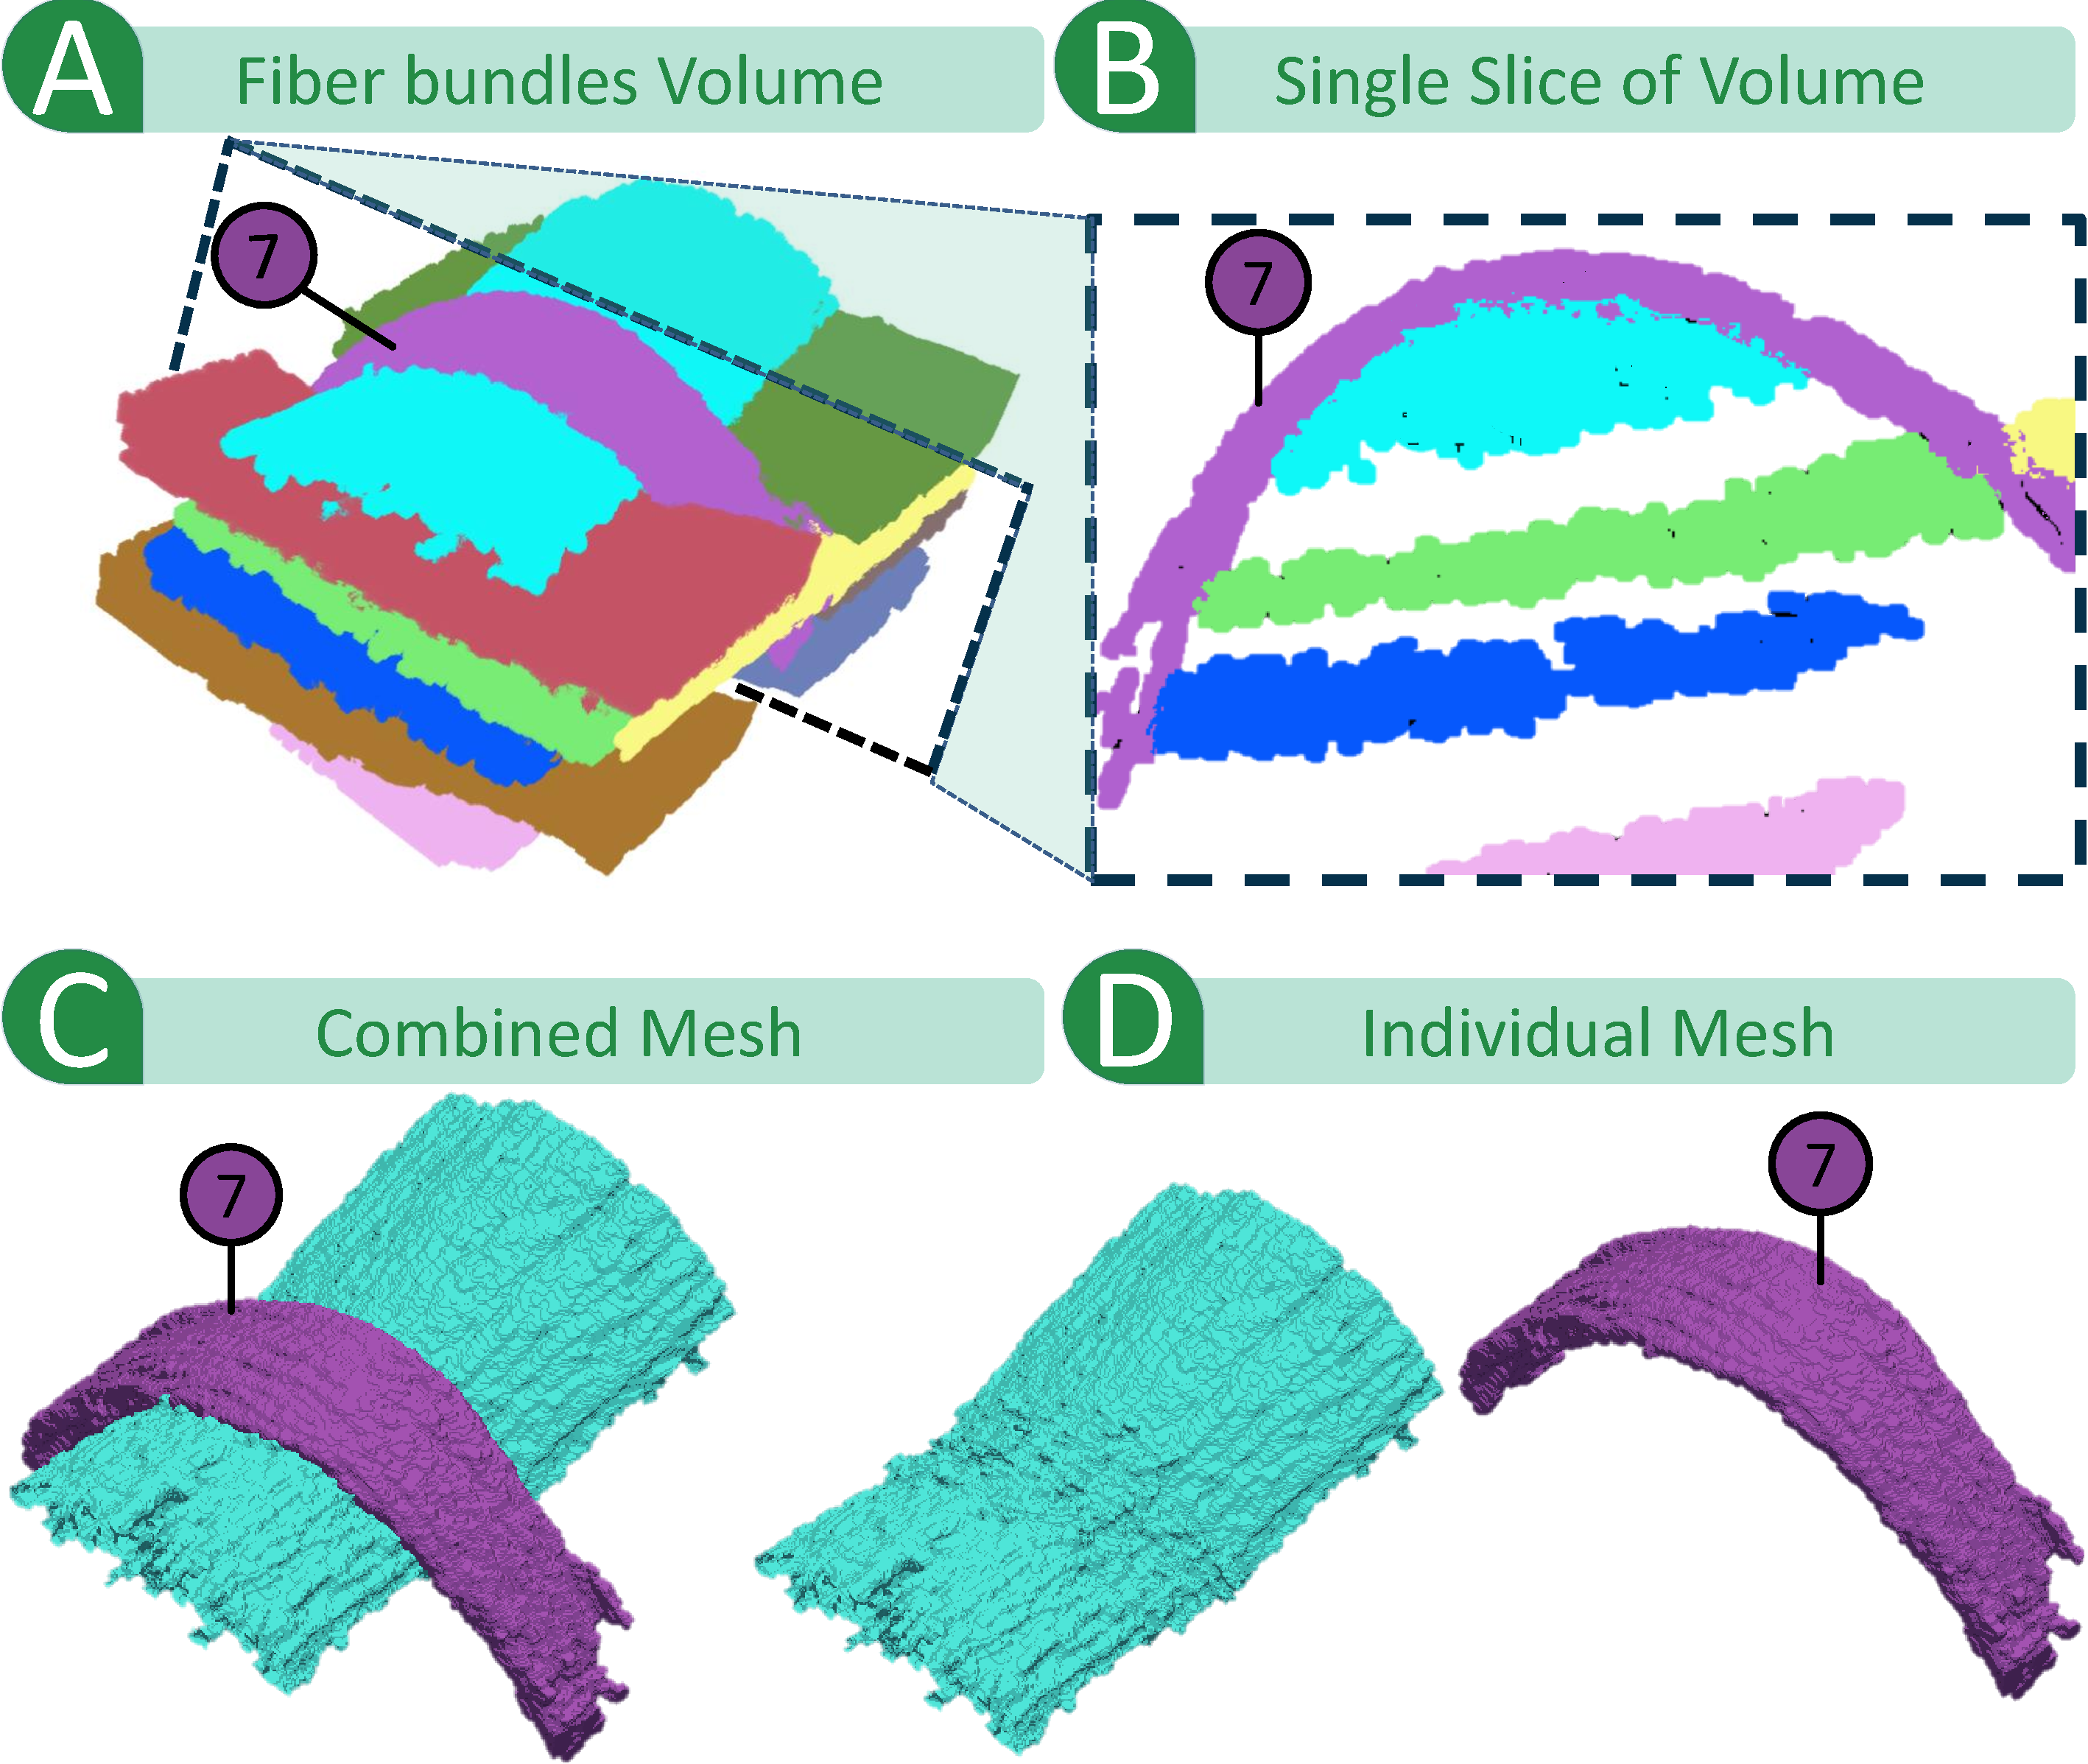
\includegraphics[width=0.4\textwidth]{images_pvis/figure7}
%		%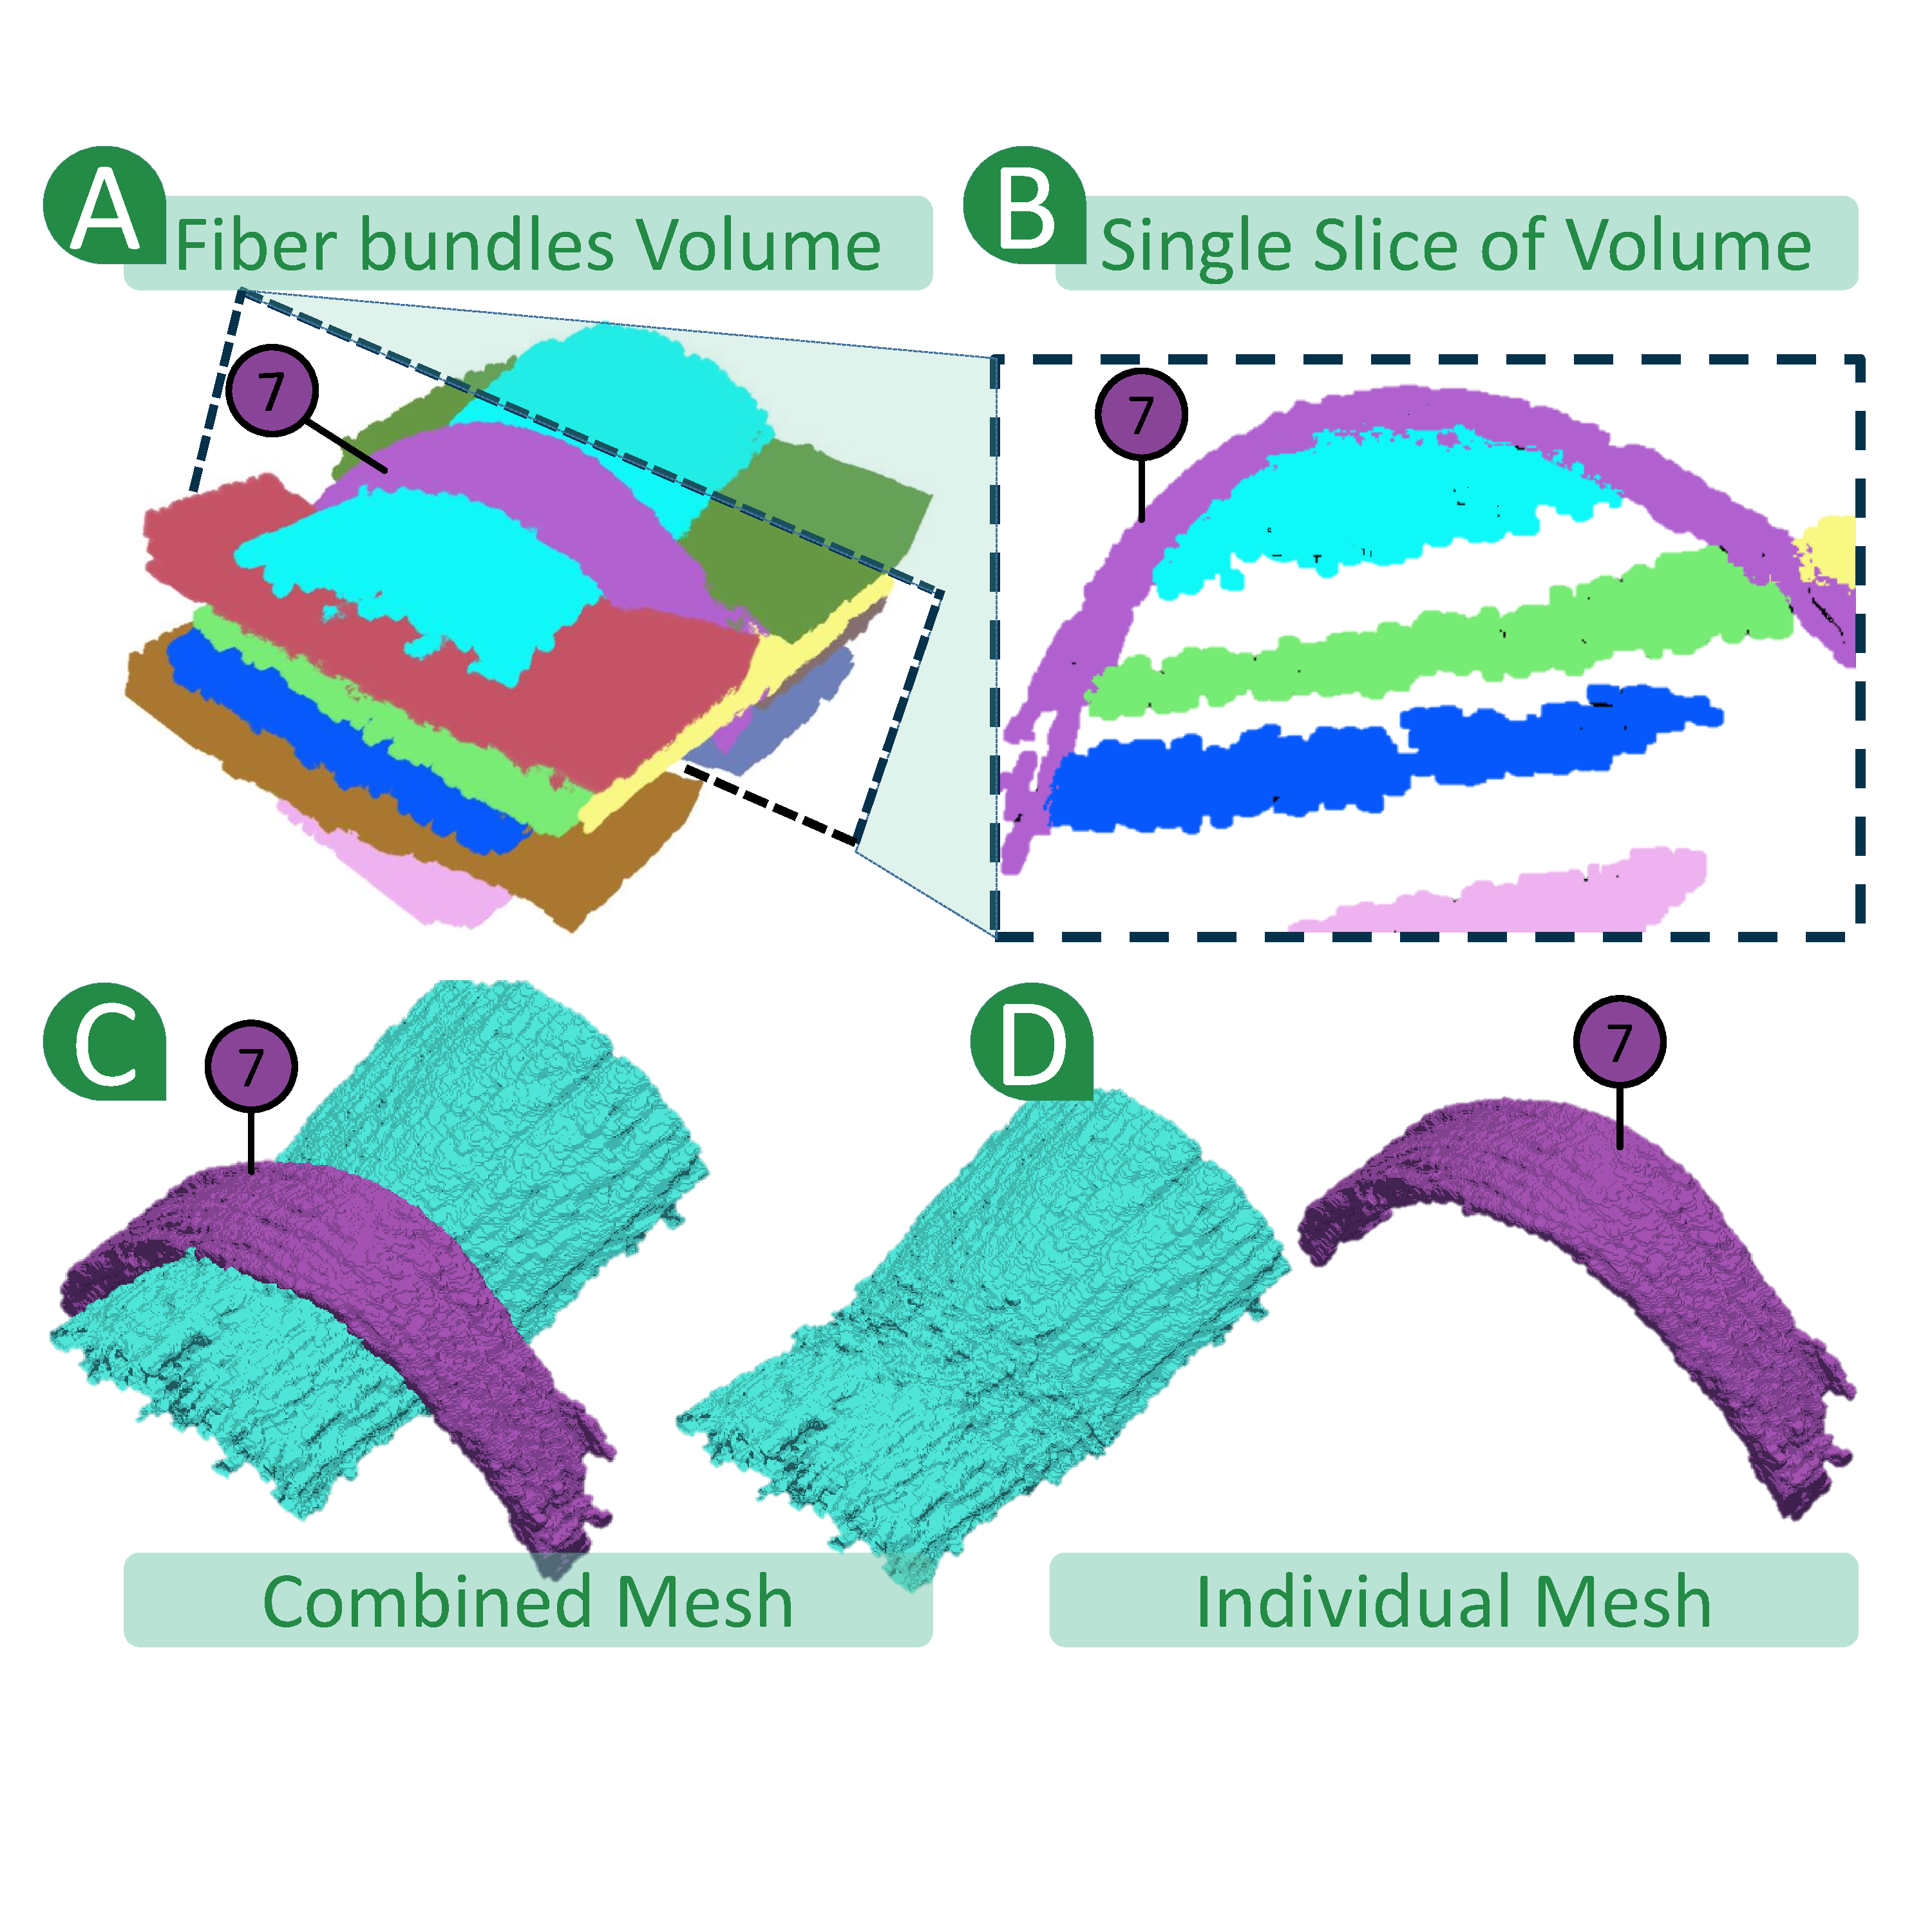
\includegraphics[width=0.5\textwidth, trim = 0mm 70mm 0mm 20mm, clip]{imagesMT2014/image7b.pdf}
%	%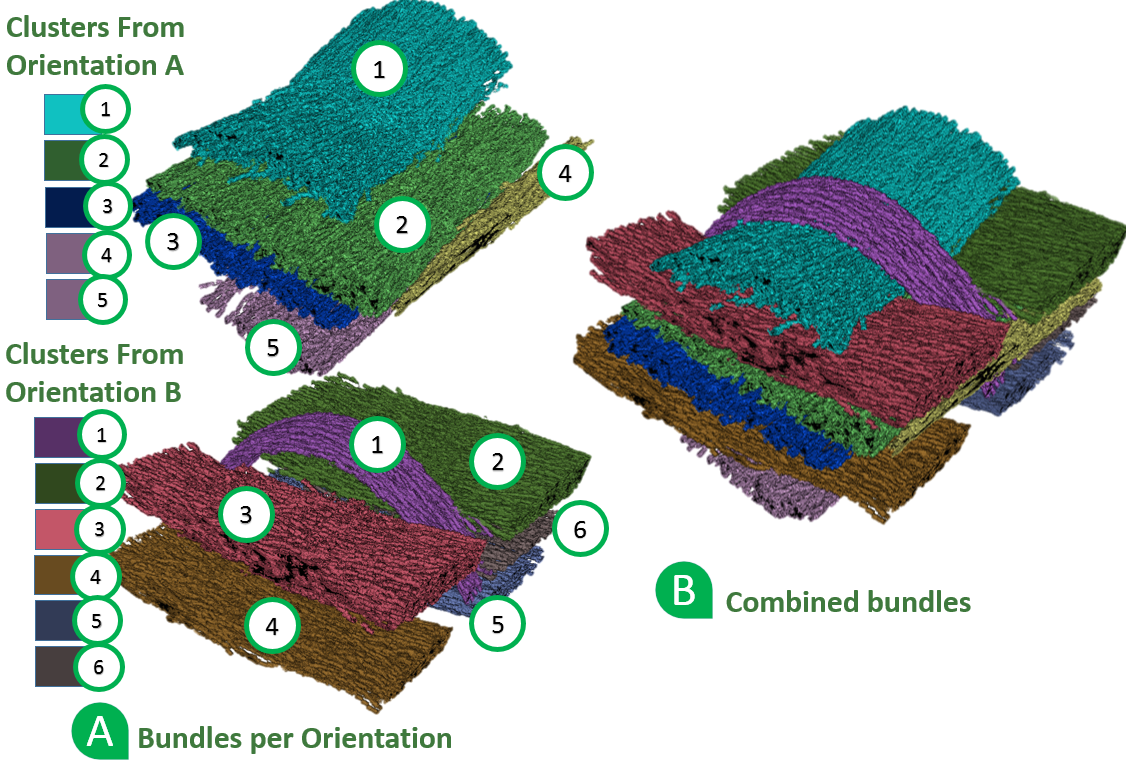
\includegraphics[width=0.45\textwidth]{imagesMT2014/crop-16/bundles}~ 
%	%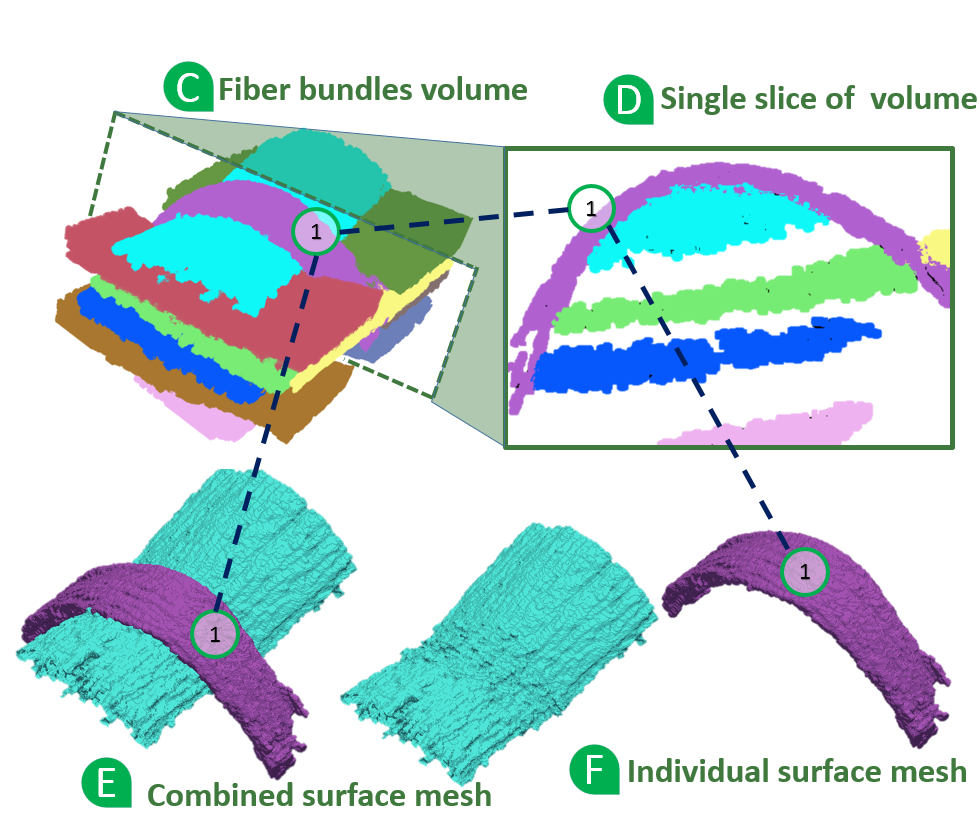
\includegraphics[height=0.35\textwidth]{imagesMT2014/crop-16/vol_mesh.png} 
%	\caption{(A) Volume rendering of data set Fig.~\ref{fig:data-char}A.(B) shows a single slice of the data set. (C) shows two of the extracted meshes together. (D) shows the meshes separately.}
%	\label{fig:crop-16-decomp}
%\end{figure}  
%  
Figure~\ref{fig:comparison}a shows the MetaTracts that are hierarchically clustered directly using proximity alone into 10, 15, and 20 clusters (ground truth is 11 clusters) without first performing orientation clustering. As discussed above, single linkage hierarchical clustering in the presence of overlapping fibers tends to create large  incorrect clusters and small(low-cardinality) outliers. When number of clusters ($h$) is 10 two large incorrect clusters are generated and the rest are outliers. As $h$ increases, some appropriate bundles start to form. Even at $h=20$, the top fiber bundles incorrectly cluster together.
%
Figure~\ref{fig:comparison}b shows the MetaTracts, clustered using K-means clustering after being embedded in a $m$-dimensional (lower) space using proximity alone, without a second hierarchical clustering step into 10, 15, and 20 clusters. In the lower dimensional space the spatial context is lost and fibers which are in reality far away are grouped together. Even at $h=20$, no correct bundles are identified.
\begin{figure}[tb]
	\centering
	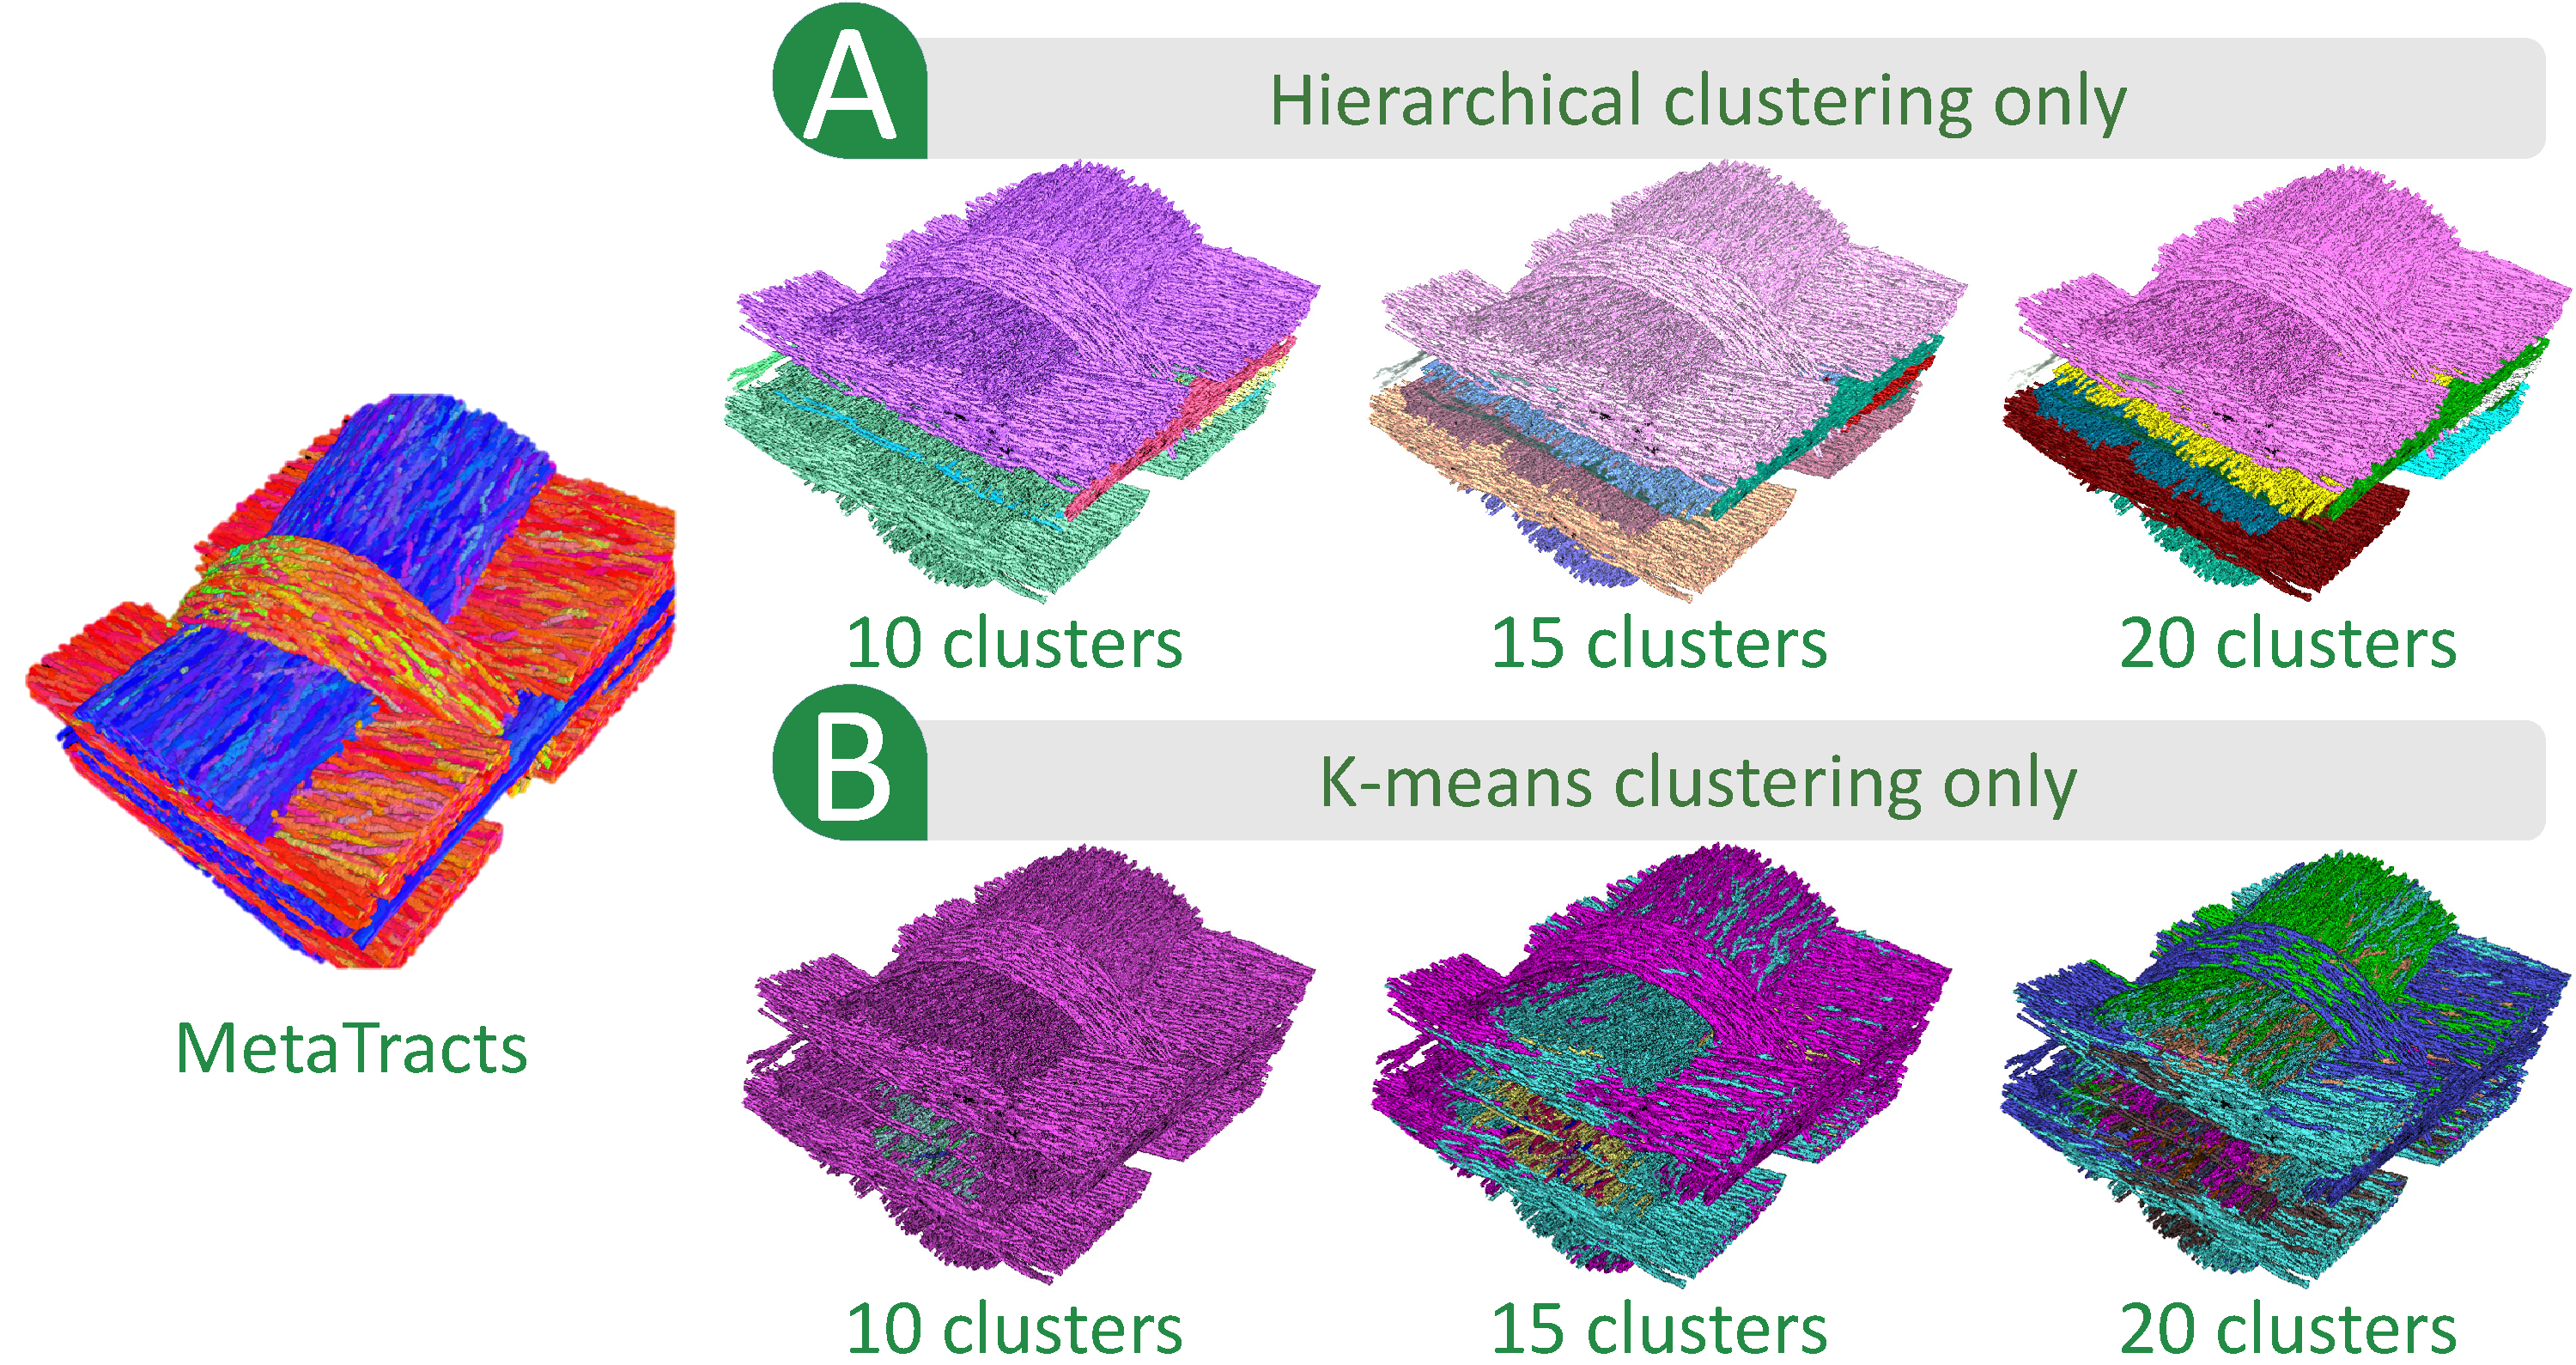
\includegraphics[width=\linewidth]{images_pvis/comparison_all.pdf}
	\caption{Applying only (a)hierarchical and (b)dimensionality reduction followed by K-means clustering methods to MetaTracts for various numbers of clusters. Using min of directed Hausdorffs as distance measure.}
	\label{fig:comparison}
\end{figure} 

% We in our approach use Zhang et al.~\cite{Zhang2008} Hierarchical clustering approach. Zhang et al.\cite{Zhang2008} define the distance between two DTI fibers Q and R as the larger mean of thresholded closest distances (equation \ref{eqn:dist}).
%In the above discussion,DTI fibers are represented as points in $\mathbb{R}^3$. MetaTracts can be correspondingly represented as points in  $\mathbb{R}^3$ in terms of the start points of the cylinders. In our implementation Q and R are sets of `$C_{p}$'s. We in our implementation set $t$ to be same radius of the cylinders for all our tests. If two MetaTracts are less than a width of the cylinder apart then they are describing the same region. We use $D_{Lt}$ as our proximity measure.
%\begin{equation}\label{eqn:dist}
%D_{Lt}(Q,R,t)= max (d_{t}(Q,R,t),d_{t}(R,Q,t))
%\end{equation} 
%where, 
%\begin{equation}\label{eqn:dist-2}
%d_{t}(Q,R,t)= mean_{a\in Q,(min_{b\in R})\parallel a-b\parallel \geq t } min_{b\in R}
%{\parallel a-b\parallel}
%\end{equation} 
%The input to this step are the results of orientation based clustering (fig.~\ref{fig:clustering}b), the figure along with our data assumptions  provides some reasoning why $D_{Lt}$ is effective in our case. The MetaTracts donot necessarily run from boundary to boundary of our data. In fig.~\ref{fig:clustering}b, "Orange", MetaTracts within the  yellow rectangle might be "diverging" (running parallel for a distance and then diverge~\cite{Zhang2008}). Also, while the MetaTracts are close at some points, they belong to different bundles. So unlike the orientation measure,  mean of closest distance $d_{t}(Q,R,t)$ is a better fit than single point comparison.
%
%Hierarchical clustering approaches have one main parameter, which is the number of clusters $h$. For each cluster extracted based on the orientation phase we cluster the result into $h$ clusters. Fig. \ref{fig:clustering} (c) shows the result from hierarchical clustering.
%
%\subsection {Notes on Clustering techniques}
%\label{subsec:other_clustering}
% The current two phase clustering technique was chosen for its simplicity, relevance to the domain understanding, intuitive nature of the parameters ($K$ and $h$, see sec~\ref{sec:param_choices}). Moberts et al.~\cite{Moberts2005} also remarks that specifying number of clusters is more intuitive than other criterias such as  number of neighbors and edge thresholds. Secondly, on average we have around ten thousand individual tracts. Solving the eigen decomposition problem for such large number of tracts in time consuming. Once the orientation clustering is completed, for each particular orientation the number of fibers being compared in less, and  hierarchical  clustering can be done in a fraction of time compared to the eigen based approach this makes the choosing of $h$ an interactive process. 


\section {Voxelization and surface extraction}
\label{sec:vis}

Apart from direct visualization of the MetaTracts, we show two additional extensions which were requested by our domain specialists as highly important. The first extension is voxelizing the original volume according to the clusters each voxel is associated with.
The second is to extract the corresponding surfaces from the voxel data by binarizing the volume per cluster and extracting the isosurface of the largest connected component from the binary volume. Both methods can possibly be used for further analysis of the data, e.g. in simulations.
%
To voxelize the space,  we compute a neighborhood around each voxel. We then enumerate the number of voxels of each class (cluster) in this neighborhood. The voxel is then assigned to the class with the maximum number of elements in the neighborhood. Figure~\ref{fig:crop-16-decomp}a and~\ref{fig:prepreg}d show the result of voxelization. Figure~\ref{fig:crop-16-decomp}c,d shows examples of extracted meshes.

\begin{figure}
\centering
		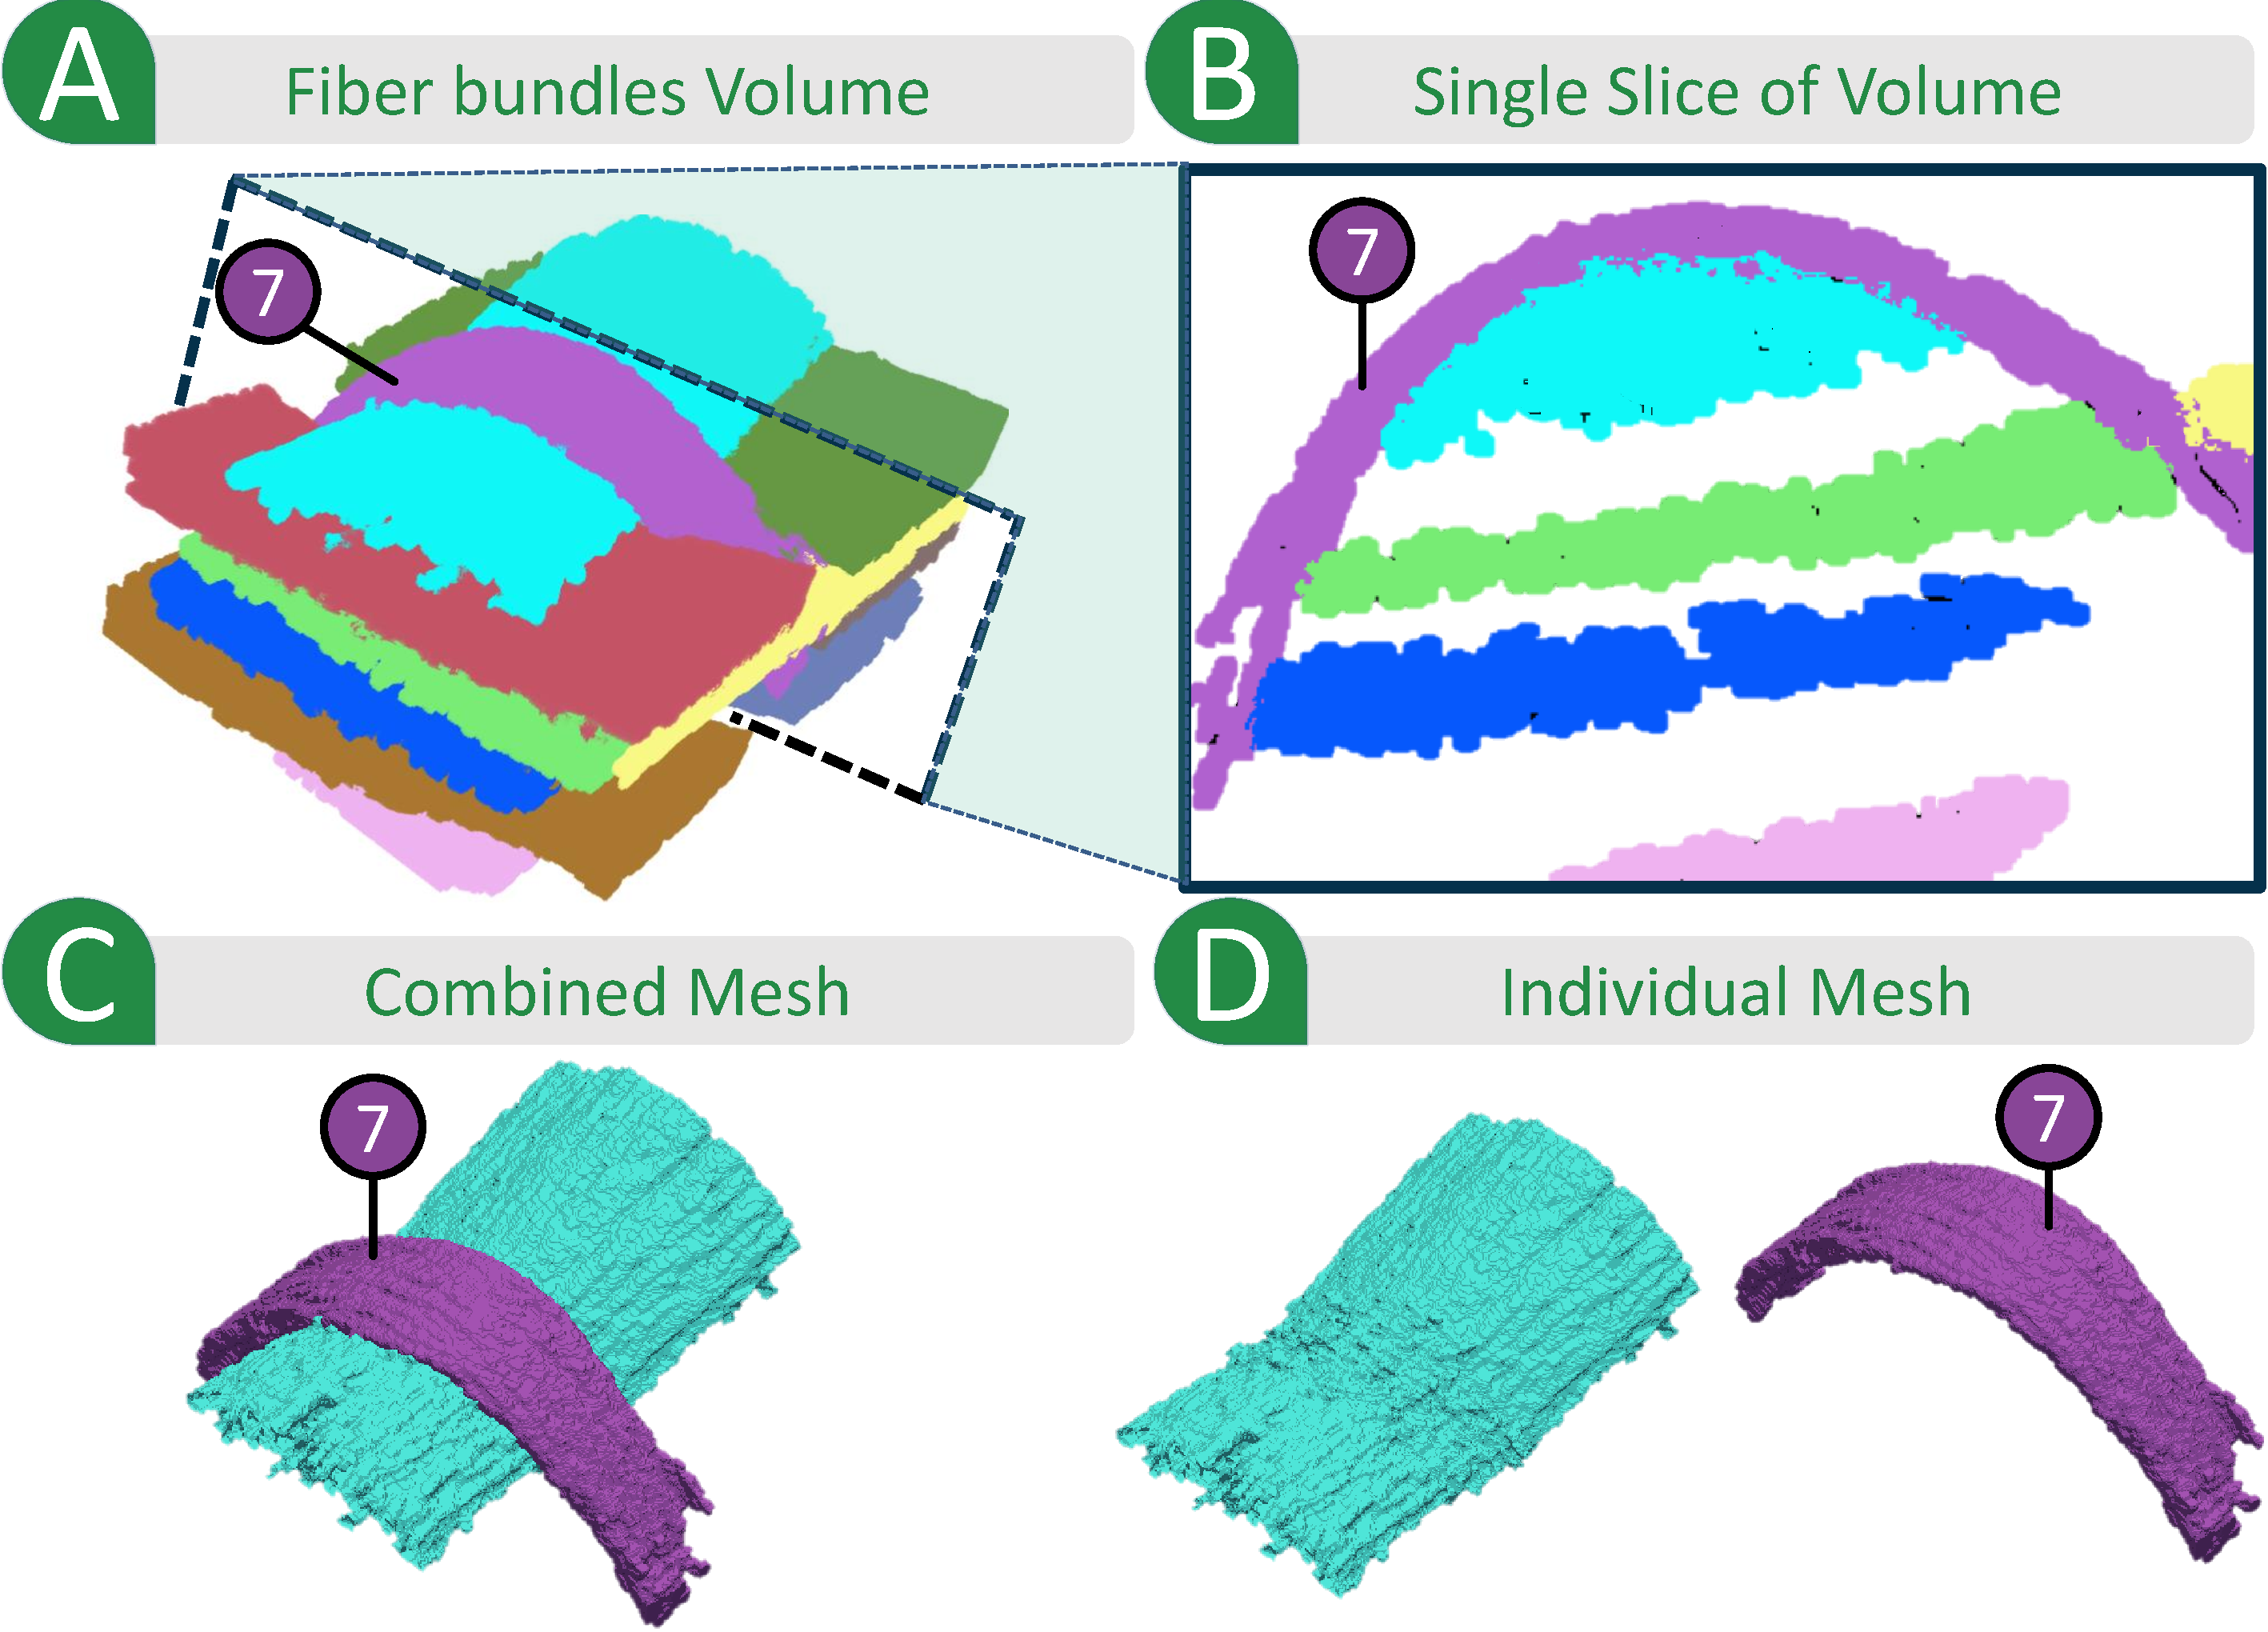
\includegraphics[width=\linewidth]{images_pvis/figure8.pdf}
		 \vspace{-1.5em}
		%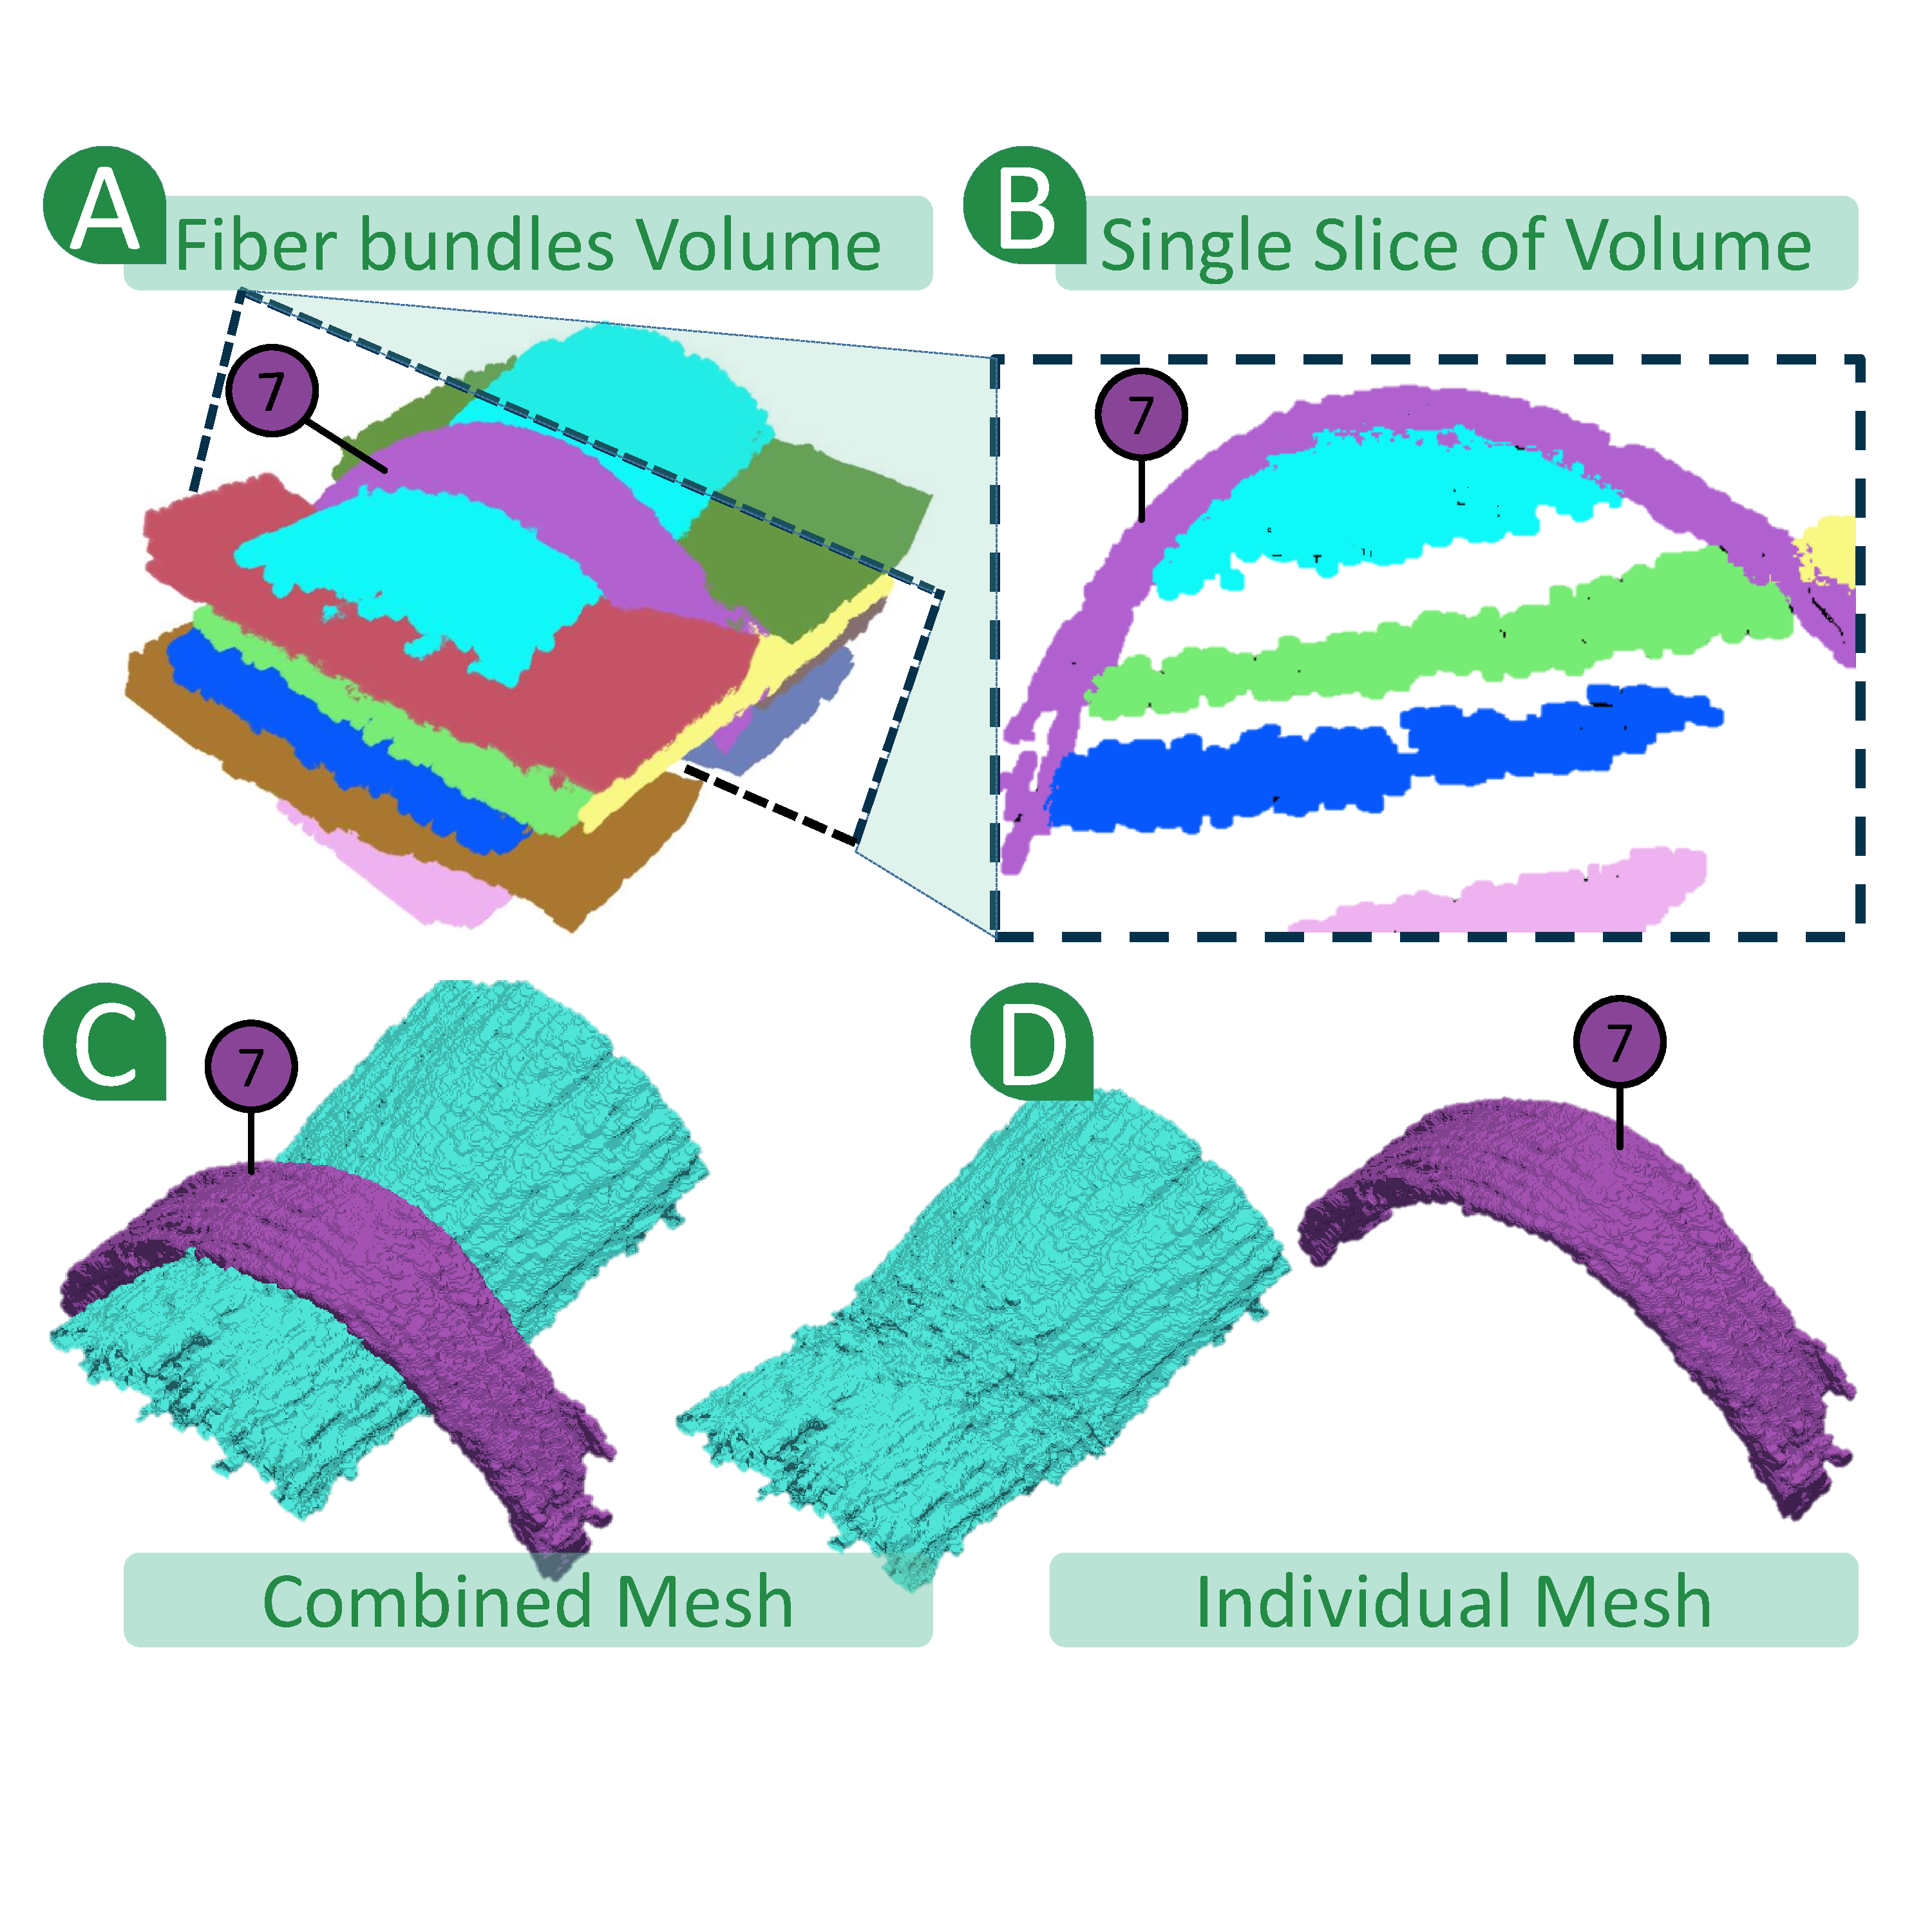
\includegraphics[width=0.5\textwidth, trim = 0mm 70mm 0mm 20mm, clip]{imagesMT2014/image7b.pdf}
	%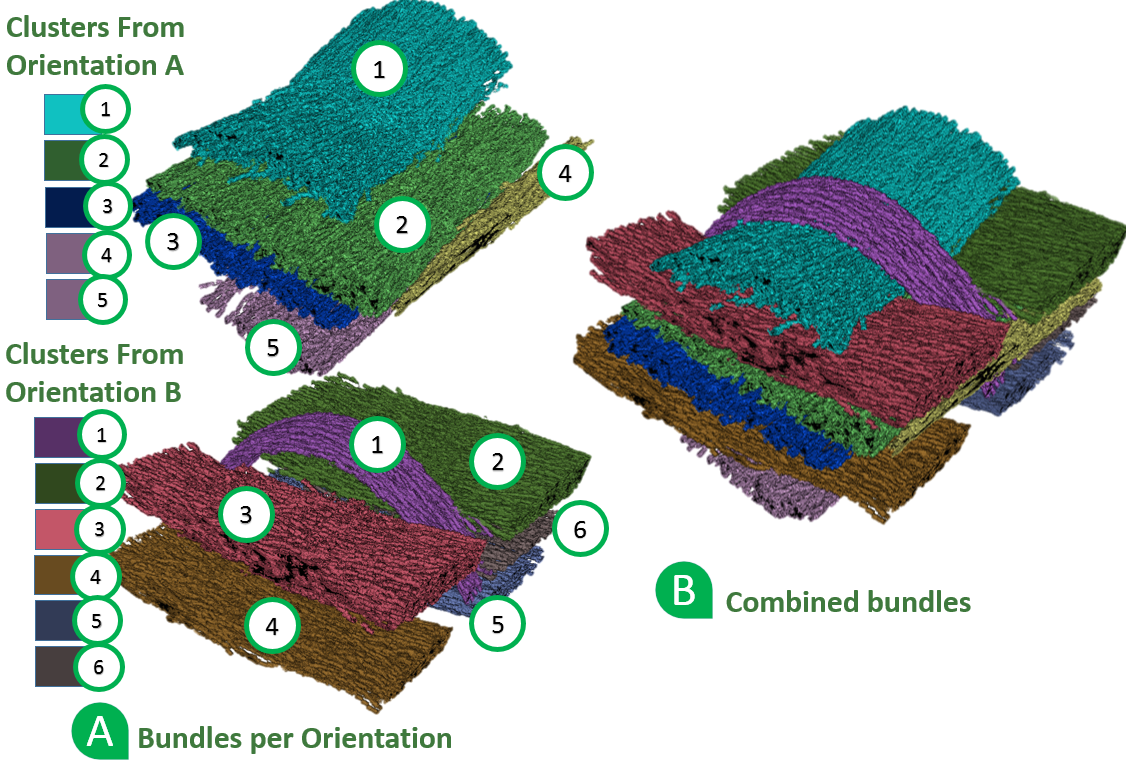
\includegraphics[width=0.45\textwidth]{imagesMT2014/crop-16/bundles}~ 
	%\includegraphics[height=0.35\textwidth]{imagesMT2014/crop-16/vol_mesh.png} 
	\caption{(a) Voxelization of data set 1; (b) a single slice of the data set; (c) two of the extracted meshes together; (d) the meshes rendered separately.}
	\label{fig:crop-16-decomp}
\end{figure}  


%The MetaTracts and the clustering provide an abstraction of the fiber bundles and are used as a visualization tool. Through visualization MetaTracts we can answer all the queries mentioned in Section~\ref{sec:intro}. 
%
%In this Section we show two simple extensions to the MetaTracts and discuss how the end user might benefit from each. One way to visualize  the bundles is to color map the original volume according to the clusters each voxels are associated with (Section~\ref{subsec:voxel}). The second is to extract the surfaces from the voxel data (Section~\ref{subsec:surf_ext}). The visualizations can be used together, for example Fig.~\ref{fig:crop-13-mesh}e shows the crossover bundle as a mesh overlay on the MetaTracts.
%
%\subsection{Voxelization}
%\label{subsec:voxel}
%
%We take the following approach for associating a voxel $v$ with one of the cluster classes. We compute a neighborhood around each voxel. We enumerate the number of voxels of each class in this neighborhood. The voxel $v$ is then assigned to the class with the maximum number of elements inside the neighborhood. In this particular implementation, we look for neighbors in a ball of radius $r$ around the voxel. Intuitively  this is a modification of the flood-fill algorithm. In practice, we observed that a suitable value of the radius is half the distance used for seeding the volume.
%More sophisticated approaches could be employed depending upon the error-tolerance of the application used. Fig.~\ref{fig:crop-13-mesh}a shows the results of applying the voxelization step to the clustering result shown in Fig.~\ref{fig:clustering}c. This adds a level of abstraction over the MetaTracts visualization and brings us closer to the declared goal of visualizing the bundles directly at individual voxel level. Clipping planes through the voxel data can then clearly show the changing sizes of cross-sections of the bundles.
%
%\begin{figure}
%  \centering
%   \subfloat[]{\includegraphics[width=0.2\linewidth]{imagesMetaTracts/crop-13voxel.eps}}
%  \subfloat[]{\includegraphics[width=0.22\linewidth]{imagesMetaTracts/crop-13-mesh-b.eps}}
%  \subfloat[]{\includegraphics[width=0.18\linewidth]{imagesMetaTracts/crop-13-mesh-a.eps}}
%  \subfloat[]{\includegraphics[width=0.21\linewidth]{imagesMetaTracts/crop-13-mesh-c.eps}}
%  \subfloat[]{\includegraphics[width=0.24\linewidth]{imagesMetaTracts/mtSurf-2}}
%  \caption{Visualization: (a) shows the voxelization. (b) shows the result of extracting surfaces from the result of the voxelization step (Clusters with very few elements have been discarded as a post processing step.), (c) and (d) shows the clusters in particular orientation direction.(e)shows the cross-over bundle as a mesh overlay on the MetaTracts. }\label{fig:crop-13-mesh}
%\end{figure}
%
%
%\subsection{Surface Extraction}
%\label{subsec:surf_ext}
%The voxelization step divides the image volume into coherent clusters. Where each voxel is associated with the cluster index of the corresponding fiber bundles. We can then use isosurfacing algorithms to find the boundaries of separation of the clustered classes. This step produces a triangular mesh following the popular marching cubes algorithm \cite{Lorensen1987}. The surfaces are computed for each of the clusters based on the voxelized grid. Our rather simple voxelization criterion means we cannot guarantee any convex or manifold criteria without adopting a more sophisticated material boundary separation algorithm.
%
%In a post processing step we remove clusters whose number of elements are far less than the mean number of elements per cluster. This simply removes outliers generated by the hierarchical clustering of classes with very few members. Fig.~\ref{fig:crop-13-mesh} shows the results of surface extraction. Fig.~\ref{fig:crop-13-mesh}b shows all the triangle meshes. Fig.~\ref{fig:crop-13-mesh}c and Fig.~\ref{fig:crop-13-mesh}d shows the meshes from two different orientation clusters. 
%Fig.~\ref{fig:crop-6} shows more results. Further processing techniques such as finding the medial axis might be applied to the extracted surface. Other NDT methods which takes meshes as input can also be utilized.


\section {Experimental Results}
\label {sec:results}
%\begin{figure*}
%\centering
%\captionsetup[subfigure]{labelformat=empty}
%	%\subfloat[]{\includegraphics[width=0.10\textwidth]{imagesMT2014/crop-6-G.PNG}}
%	%\subfloat[]{\includegraphics[width=0.10\textwidth]{imagesMT2014/crop-6-H.PNG}}
%	%\subfloat[]{\includegraphics[width=0.35\textwidth]{imagesMT2014/crop-6-I.PNG}}
%	
%	\subfloat[(a) Dat set 2]{\includegraphics[width=0.7\linewidth]{imagesMT2014/prepreg/Capture8.PNG}}
%	\subfloat[(b) Data set 3]{\includegraphics[width=0.2\linewidth]{imagesMT2014/dataset203.png}}	
%	\caption{(a) Shows in order, the volume rendering of the second data set, a single (2D) slice, the orientation clustering bundles and the final bundles followed by proximity clustering. (b) Shows in order the third data set, a single (2D) slice and finally the extracted fiber bundles.}
%	\label{fig:crop-6}
%\end{figure*}

\begin{figure}[tb]
\centering
	%\includegraphics[width=0.45\textwidth]{imagesMT2014/image8b}
	\includegraphics[width=\linewidth]{images_pvis/dataset2.pdf}
	\caption{Data set with flat thin and compact bundles. (a) shows the volume rendering and a 2D slice with one of the boundaries marked in green, (b) shows the clusters according to individual orientation. (c) shows the complete result. (d) shows the voxelization of (c).}
	\label{fig:prepreg}
\end{figure}

%Fig~\ref{fig:kull} (b) shows the results after the MetaTracts extraction. Fig.~\ref{fig:kull} (c) shows the results of the orientation clustering with $K$ set to 2. Note, that the curved fiber bundle has also been detected with the correct orientation. Fig. \ref{fig:kull} (d) and (e) shows the results of hierarchical clustering of \ref{fig:kull} (c) using proximity based clustering. Both the orientation were clustered into 14 classes.

 %glass
We tested our method on three datasets with varying characteristics. We report results on two here and third in the supplemental section.  
Dataset 1 is described in Sec.~\ref{sec:char_data} (Figure~\ref{fig:data-char}). Dataset 1 has eleven separate fiber bundles (5 along one orientation and 6 along the other). All of them were identified correctly by MetaTracts. With different cross-section sizes and varying degree of curvature of the bundles, dataset 1 is a complicated dataset.
Figure~\ref{fig:orientation_clustering} and Figure~\ref{fig:crop-16-decomp} shows the result of dataset 1 decomposed into two orientation clusters with each orientation cluster further decomposed into $h=10$ clusters followed by voxelization and mesh extraction. Note how the thin and curved purple cluster bundle 7 is extracted well (Figure~\ref{fig:orientation_clustering}e, Figure~\ref{fig:crop-16-decomp}d). 

Figure~\ref{fig:len_dist_crop16} shows the median, minimum and maximum lengths per cluster in orientation 1 (Figure~\ref{fig:orientation_clustering}d) clustered into 10 clusters, the ground truth being  5 clusters. We generate the correct clusters and outlier bundles with very few elements which can be discarded. As noted in Sec.~\ref{subsec:dist_clustering}, the MetaTracts do not run the entire length of the dataset, the median length of MetaTracts in cluster six (Figure~\ref{fig:len_dist_crop16}) is 200 while the maximum MetaTract length in the bundle is about 500 (measured in units of grid cube length: 2 $\mu m$). Figure~\ref{fig:length_distribution}b shows the length per MetaTract distribution for a particular fiber bundle. 

Figure~\ref{fig:prepreg} shows the results on our dataset 2. This dataset has different characteristics, and is dense with \textit{flat and thin} bundles, it consists of 4 bundles along one direction and 5 along the other. The dimensions are 300$\times$350$\times$300 and the datatype is uint16 (dataset 1 is uint8). The bundles are indistinguishable in the original data set Figure~\ref{fig:prepreg}a. A green dotted line shows one of the fiber bundle boundary. Figure~\ref{fig:prepreg}b shows the fiber bundles for the two orientations, Figure~\ref{fig:prepreg}c shows the combined results, and Figure~\ref{fig:prepreg}d shows the volume after the voxelization.

The fiber bundle extraction using MetaTracts was implemented in C++ using ITK. All clustering was done in R. The preprocessing is time consuming and may take several hours. It consists of MetaTract generation and the distance computation. The orientation clustering is robust and done as a part of preprocessing. The hierarchical clustering by itself, on the results of the orientation clusters can be done within an order of a few minutes on Intel Xeon E5-2667 workstation and can be repeated according to user input of $h$ (Sec.~\ref{sec:param_choices}). We store the normalized direction at each fiber point, thus both distance measures can be extracted simultaneously without any extra computations.



\section {User Evaluation}
\label {sec:user_eval}
\begin{figure}[tb]
	\centering
	\includegraphics[width=\linewidth,  trim = 0mm 00mm 0mm 0mm, clip]{images_pvis/usereval_AMA.pdf}
	%\includegraphics[width=0.5\textwidth,  trim = 10mm 40mm 0mm 15mm, clip]{imagesMT2014/image_length_histogram.pdf}
	\caption{The user evaluation consists of a set of queries on videos of our results, volume rendering and Hessian colormap. The questionnaire tests the effectiveness of MetaTracts in visualizing ``geometric structure" and ``spatial context". The Likert scale goes from 1-5: strongly disagree, disagree, neutral, agree and strongly agree. }
	\label{fig:userstudy}
\end{figure}
Four NDT practitioners who are familiar with X-Ray computed tomography and its visual representations, four material scientists who are experienced in analyzing fiber reinforced polymers and four practitioners of visualization participated in the user evaluation of our work. We setup a questionnaire with questions on solving given tasks as well as questions using the Likert scale (LS) for evaluating the performance of the MetaTracts over currently used techniques. LS consists of 5 levels from ``strongly disagree" to ``strongly agree". Figure~\ref{fig:userstudy} shows the results in the sequential order they were asked. Task 1 of the questionnaire was to ``identify the number of fiber bundles" from a video showing a 360 degree rotation of the volume rendering of dataset 1 (Figure~\ref{fig:data-char}a). This task tests the perception of geometric structure and how common problems like uniform grayscale values and occlusion of the different fiber bundles affects the user. Figure~\ref{fig:userstudy} shows that, as expected the participants found it difficult to determine the number of bundles from volume rendering alone. Another common approach is to color map the top eigenvector of Hessian matrix to RGB space. We show a video showing a 360 degree rotation of the volume rendering of the color mapped eigenvectors (similar to Figure~\ref{fig:reliable_hessian}a) and asked the same query. Compared to the volume rendering, the Hessian color map provides more information about the major orientations and we see that the evaluators performed better in this test than in the direct volume rendering test. The majority of our participants agreed or strongly agreed (LS) that Hessian color map was more effective. Finally, we showed the MetaTracts extracted bundles (for orientation 1 and 2 separately Figure~\ref{fig:orientation_clustering}d,e). All participants could correctly identify the number of fiber bundles. All participants agreed that MetaTracts was more effective in perceiving geometric structure than direct volume rendering. They especially liked the two dimensional slices of the MetaTracts (Figure~\ref{fig:crop-16-decomp}b, compared to Figure~\ref{fig:data-char}c).
The next set of tasks on the MetaTracts results tests the spatial context perceived from MetaTracts. We achieve this by asking the evaluators to select the largest fiber bundle from a subset of fiber bundles, to select the smallest from a subset and given a fiber bundle and to select the most similar one from a subset. Due to the problems of occlusions and similar grayscale values these tests are difficult on volume rendering of the plain data only, but straight forward using MetaTracts. In the Likert scale, the majority strongly agreed that the tasks are undemanding compared to volume rendering.
Finally, the majority participants agreed that the extracted meshes provides better spatial context than volume rendering. 
 
\section{Parameter choices}
\label{sec:param_choices}
\begin{figure}[tb]
\centering
	\includegraphics[width=\linewidth,  trim = 0mm 0mm 0mm 00mm, clip]{images_pvis/figure9_AMA.pdf}
	 \vspace{-1.5em}
	%\includegraphics[width=0.5\textwidth,  trim = 10mm 40mm 0mm 15mm, clip]{imagesMT2014/image_length_histogram.pdf}
	\caption{Number of tracts and median, minimum and maximum length of individual MetaTracts in the orientation cluster Figure~\ref{fig:orientation_clustering}d, clustered into 10 clusters. The unit for length is the grid cube length.  Clusters labeled 2,3,4,5 and 7 all have cardinality less than 10. }
	\label{fig:len_dist_crop16}
\end{figure}
The critical parameters are $K$ for the K-means in orientation based clustering and $h$ for the hierarchical clustering. K denotes the number of major directions, which is either known a priori or can be easily estimated by looking at the weaving pattern. 
Our framework is robust to the choice of $h$. Large $h$ keeps the major bundles intact. For example, in  Figure~\ref{fig:len_dist_crop16}, where $h$ was set to ten while the ground truth was five clusters, we observe that the major clusters remain well segmented and small clusters can be removed if they have too few elements (clusters 2,3,4,5 and 7 in Figure~\ref{fig:len_dist_crop16} all have less than 10 elements). This is an appealing trait of the proximity based clustering, thus providing good results even when exact $h$ might be unknown (avoiding over-segmentation).
The following parameters were fixed for all the tests. We set the reliable Hessian threshold $R_{H}$ to be 0.3 for all our tests. A $R_{H}$ of 0.0 would mean all points have reliable local orientation which would cause spurious MetaTracts detection. A very high $ R_{H}$ would lead to a decline in number of MetaTracts produced. The $\alpha$ and $\beta$ in $R_{H}$ are as explained in Frangi et al. \cite{Frangi1998} and set to 0.5. The length and the radius parameters for the cylinders of MetaTracts decide how coarse the fiber cylinders are. These are dependent on the underlying fiber characteristic and the weaving pattern. Larger cylinders will handle noisy local orientation better as it inspects a higher number of candidate points to extend the fiber. We used 10.00 and 2.00 for length and radius (measured in grid voxel size), respectively for all tests.  
Simpler geometry (example dataset 2) was experimentally found to handle larger cylinders better. $\eta$ in sec.~\ref{subsec:dist_clustering} decides how quickly the hierarchical clustering converges, experimentally 0.3 to 0.6 gave similar results. 
 %Short tracts of less than 0.01 times the smallest axes size are prone to have erroneous local orientation and are therefore removed. 
 $\alpha$ and $\beta$ in equation~\ref{eqn:algo_1} decide how quickly the value of the factor decays; we have used [7-10] and half the length of cylinder (5.0). Our number of fiber bundle directions are limited. Thus even for small $m$ (cardinality of lower dimension in orientation clustering), the distinction between the orientation clusters is preserved quite well. We compared  $m=3-7$ experimentally without any change in results. 
%\begin{figure}[tb]
%	\centering
%	\includegraphics[width=0.5\textwidth, trim = 0mm 80mm 0mm 170mm, clip]{images_pvis/figure10}
%	\caption{Direct hierarchical clustering of MetaTracts Fig.~\ref{fig:length_distribution}(A) by proximity into 10,15 and 20 clusters.}
%	\label{fig:comparison}
%\end{figure}
%

 

%\begin{figure}
%\centering
% \subfloat[$\eta=7$]{\includegraphics[width=0.3\linewidth]{imagesMetaTracts/Rplot-ndim3k2}}
%  \subfloat[$\eta=3$]{\includegraphics[width=0.3\linewidth]{imagesMetaTracts/Rplot-ndim7k2}}
%  \caption{Embedding from $\mathbb{R}^m\to \mathbb{R}^\eta$, here m is the number of MetaTracts, 580 for this example. Followed by clustering into K=2 clusters.}
%  \label{fig:eta}
%\end{figure}
%\begin{figure}[htp]
%\centering
% \includegraphics[width=\linewidth]{imagesMetaTracts/kul-results.eps}
%  \caption{Results from orientation based dimensionality reduction and clustering. A is the original data set, B shows the results of fiber tracking. C shows the results of orientation based clustering and D shows the results of the proximity based clustering. }\label{fig:kull-full}
%\end{figure}

%\begin{figure}[htp]
%\centering
% \includegraphics[width=\linewidth]{imagesMetaTracts/glass-clus-2.eps}
%  \caption{ Fig  A and C shows the results fiber extraction. B and D shows the results of clustering with clipping planes.}\label{fig:closeup-full}
%\end{figure}


\section{Limitations and future work}
\label{sec:conclusions}
\color{red}
 A key assumption of the method is ``connectivity'' (Sec.~\ref{sec:char_data}).
If the ``connectivity'' is not satisfied due to noise in the image, the then MetaTracts will be inaccurate. 
The clustering process also assumes that the fiber bundles have a minimum width.
\color{green}
In this paper, we introduce a framework to extract and visualize fiber bundles in composite materials. We show that our framework works at comparatively low resolution and with dense fiber arrangements (when extracting single fibers might not be possible). It handles complex fiber patterns such as ``cross overs'' and ``braiding''. We perform an user evaluation to indicate the usefulness of the method.
\color{black} In future, we plan to increase the precision of the extractions, include uncertainty based visualization to better portray the surface of separations and speed up extraction times.
%
%\begin{figure}
%  \centering
%  \subfloat[]{\includegraphics[width=0.2\linewidth]{imagesMetaTracts/crop-6-scalar.eps}}
%  \subfloat[]{\includegraphics[width=0.2\linewidth]{imagesMetaTracts/crop-6-tracks-1.eps}}
%  \subfloat[]{\includegraphics[width=0.2\linewidth]{imagesMetaTracts/crop-6-tracks-clus-a.eps}}
%    \subfloat[]{\includegraphics[width=0.2\linewidth]{imagesMetaTracts/crop-6-tracks-clus-b.eps}}
%  \subfloat[]{\includegraphics[width=0.2\linewidth]{imagesMetaTracts/crop-6-labels-all.eps}}
%  \caption{Dense data set with bundles which are flat and thin. (a) shows the results original dataset, (b) shows the results of metaTract extraction, (c) shows the results of our two step clustering  into 14 classes. (d) shows the results of voxelization  and (e) shows the results of surface extraction. }\label{fig:crop-6}
%\end{figure}
%% if specified like this the section will be ommitted in review mode


\acknowledgements{
The research leading to these results has received funding from the European Union’s Seventh Framework Programme (FP7/2007-2013) under grant agreement ACP2-GA-2012-314562-QUICOM. Our special thanks go to Ilya Ilya Straumit (KU Leuven) who provided us with dataset1.
}
